\documentclass[TS]{sesamanuel}

% modifications dans la classe (fichier sesamanuel.cls) :
% 	1) ligne 2873, la ligne de remise à zéro du compteur de chapitre a été commentée pour "themaG"
% 	2) création d'une boîte à connaître à la ligne 3471
%	3) ligne 2141 : définition de trois couleurs utilisé par les anciennes figures libreoffice
%	4) ligne 179 et 180 ajout de 2 lignes pour utiliser la police pazocal qui modifie les caractères calligraphiés en mode math
%		du coup : \mathcal{C} donne un C fortement calligraphié et \pazocal{C} donne l'habituel C calligraphié de mathcal

% modifications dans le fichier commandesTikZ :
% lignes 31 et 32 pour ajouter la commande \circled qui entoure un caractère


% a priori, après l'impression du livre, tout ce fichier devrait être
% fusionné avec la classe principale, dernière version

\AtBeginDocument{\color{Noir}}

\renewcommand*\StringPrerequis{Connaissances
  n\'ecessaires \`a ce chapitre}

\usepackage{textcomp,pgfplots}
% standalone ne gère pas graphicspath... hum...
\newcommand{\standalonepath}[1]{#1}
% Au début de chaque chapitre on redéfinira cette commande en
% indiquant le chemin

\frenchbsetup{og=«,fg=»,}

\renewcommand\PrefixeCorrection{Corrections/}
\DeclareRemLike{intuition}{Idée intuitive}
\DeclareRemLike{exemples}{Exemples}


\newcommand*\StringExemples{Exemples}
\makeatletter
\newcommand*\smc@cartoucheexemples{% au pluriel
  \begin{pspicture}(-\ExempleVRuleWidthFrame,0)
                 (\ExempleWidthFrame,\ExempleHeightFrame)
    \psframe*[linewidth=0pt,linecolor=ExempleEdgeFrameColor]
             (-\ExempleVRuleWidthFrame,-\ExempleHRuleWidthFrame)
             (\ExempleWidthFrame,\ExempleHeightFrame)
    \psframe*[linewidth=0pt,linecolor=ExempleBkgFrameColor]
             (0mm,-0mm)(\ExempleWidthFrame,\ExempleHeightFrame)
    \rput[B](\dimexpr\ExempleWidthFrame/2,0){%
      \ExempleTitleFont
      \textcolor{ExempleTitleColor}{\StringExemples}%
    }
  \end{pspicture}%
}

\newenvironment{exemples*1}[1][]{%
  \par\addvspace{\BeforeExempleVSpace}
  \let\correction\smc@one@exemplecorrection
  \let\itemize\smc@exempleitemize
  \let\enditemize\endsmc@exempleitemize
  \let\colitemize\smc@exemplecolitemize
  \let\endcolitemize\endsmc@exemplecolitemize
  \let\enumerate\smc@exempleenumerate
  \let\endenumerate\endsmc@exempleenumerate
  \let\colenumerate\smc@exemplecolenumerate
  \let\endcolenumerate\endsmc@exemplecolenumerate
  \let\partie\smc@nopartie
  \let\exercice\smc@noexercice
  \let\endexercice\endsmc@noexercice
  \let\corrige\smc@nocorrige
  \let\endcorrige\endsmc@nocorrige
  \def\smc@currpart{Exemple}%
  \hspace*{\dimexpr \SquareWidth*3}%
  \color{ExempleRuleColor}%
  \vrule width \RuleWidth
  \hspace*{\dimexpr \SquareWidth-\RuleWidth}%
  \minipage[t]{\dimexpr\linewidth-\SquareWidth*4-\ExtraMarginRight}
    \smc@cartoucheexemples
    \space
    \color{Noir}%
    \ignorespaces
}
{%
  \endminipage
  \par
}

\DeclareRemLike{consequence}{Conséquence}
\DeclareRemLike{rappel}{Rappel}
\DeclareRemLike{valeurspart}{Valeurs particulières}
%\DeclareRemLike{theoreme}{Théorème}
% \NewThema{SP}
%          {sp}
%          {stat. et probabilités}
%          {Stat. et probabilités}
%          {STATISTIQUES\\ PROBABILITÉS}
%          {PartieStatistique}
%          {PartieStatistique}

\NewThema{A}
         {a}
         {analyse}
         {Analyse}
         {ANALYSE}
         {PartieFonction}
         {A3}


% Attention, il faudra ajouter un renewcommand \ListeMethodesThemes
% pour afficher la liste des méthodes à la fin du livre

% Si ils veulent changer la couleur du numéro des exos des
% auto-évaluations il faudra aller voir
% \colorlet{CorrigeNumExerciceFrameBkg}{J1}
 
\newcommand{\N}{\mathbb{N}} 
\newcommand{\R}{\mathbb{R}}
\newcommand{\Z}{\mathbb{Z}}
\renewcommand{\cfrac}[2]{{\displaystyle\frac{%
  \vrule height10pt depth0pt width0pt #1}{#2}}%
  \kern-\nulldelimiterspace}
%\usepackage{casio-fx,ti83symbols}

\newcommand\renvoimethode[1]{%
  Méthode \ref{#1}, p.~\pageref{#1}%
}

\newcommand*\calculatrice{%
  \psframebox[framesep=1pt,linewidth=\LogoLineWidth,
              linecolor=TiceLineColor, fillstyle=solid,
              fillcolor=TiceBkgColor, framearc=0.6]{%
    \TiceFont
    \textcolor{TiceTextColor}{CALC}%
  }
}
\newcommand\calc{\calculatrice}

% Chapitre G1 et G3
\newcommand{\covec}[2]{\left(\begin{array}{c} #1\\#2\end{array}\right)}

% Chapitre G2
\usepackage{tipa}
\newcommand{\arc}[1]{%
  \setbox9=\hbox{#1}%
  \ooalign{\resizebox{\wd9}{\height}{\texttoptiebar{\phantom{A}}}\cr#1}}

% Chapitre A4


\DeclareMathOperator{\e}{e}
\renewcommand{\cosh}{\operatorname{ch}}
\renewcommand{\sinh}{\operatorname{sh}}
\renewcommand{\tanh}{\operatorname{th}}

\newcommand*{\StringLEMM}{LEMME\footnote{Un \MotDefinition{lemme}{} est un résultat préliminaire ou  intermédiaire qui intervient parfois dans la preuve d'un théorème lorsqu'elle est un peu longue.}}
\newcommand*{\StringLEMME}{LEMME}
\DeclareDefLike{lemme}{\StringLEMME}
\DeclareDefLike{lemm}{\StringLEMM}

\newcommand*{\StringPROPRIETA}{PROPRIÉTÉ (admise)}
\DeclareDefLike{proprieta}{\StringPROPRIETA}

\usepackage{wrapfig}

% Environnement général pour toutes les fiches
\newcommand\AnnexeTICE{%
  \ChangeAnnexe{C2}{A1}{G1}{Blanc}%
  \annexe{}%
}
% Déclaration de l'environnement pour une fiche
\DeclareTPLike{ficheTICE}{Fiche}
              {TPTopColor}
              {TPBottomColor}
              {TPTitleColor} 
% Définition d'une commande \souspartie pour les besoins de la fiche
% TICE. C'est la commande \partie un peu revue. Je crée les mêmes
% paramètres de contrôle que pour TPPartie en mettant TPSousPartie à
% la place.

\colorlet{TPSousPartieColor}{J1}
\colorlet{TPSousPartieBkgColor}{C2}
\colorlet{TPSousPartieNumColor}{Blanc}
\newcommand*\TPSousPartieFont{\fontsize{10}{12}\sffamily\bfseries}
\def\BeforeTPSousPartieVSpace{3mm plus1mm minus1mm}
\def\AfterTPSousPartieVSpace{0mm plus1mm}
\edef\TPSousPartieHSep{\the\dimexpr\ItemRuleWidth+1.5mm}

\newcommand*\souspartie[1]{%
  \colorlet{smc@curr@partiecolor}{TPSousPartieNumColor}%
  \colorlet{smc@curr@partiebkgcolor}{TPSousPartieBkgColor}%
  \let\smc@curr@partiefont\TPSousPartieFont
  \par\addvspace{\BeforeTPSousPartieVSpace}
  \leavevmode
  \psframe*[linecolor=smc@curr@partiebkgcolor]
           (0,\ItemRuleDepth)(\ItemRuleWidth,\ItemRuleHeight)
  \hspace*{\TPSousPartieHSep}%
  \textcolor{TPSousPartieColor}{\TPSousPartieFont #1}
  \par\nobreak\addvspace{\AfterTPSousPartieVSpace}
}%

\newcommand\RoseItalTice[1]{\emph{\textcolor{C2}{#1}}}

%%% La présentation d'un texte en vis à vis d'une image n'est pas tout
%%% à fait un habillage et la répétition de tels éléments risque de
%%% poser des problèmes. Il vaut mieux se faire son propre « habillage
%%% »
\newcommand\ImageDroite[2]{%
  % #1 = texte
  % #2 = image (ou autre)
  \setbox4=\hbox{#2}%
  \dimen4=\dimexpr\ht4+\dp4-0.7\baselineskip
  \par
  \begin{tabularx}{\linewidth}{@{}Xc@{}}
    #1 & \raisebox{-\dimen4}{#2} %\box4
  \end{tabularx}
  \par
}
\newcommand{\commandetice}[1]{%
  \bgroup
  \shorthandoff{;:!?}%
  \texttt{#1}%
  \egroup
}

\newcommand\touchecalc[1]{%
  \tikz[baseline=-0.5ex]{\node at (0,0) [rounded corners = 2pt, draw, line width=.25pt]
    {\footnotesize\textsf{#1}}}%
}

\DeclareFontFamily{U}{tipa}{}
\DeclareFontShape{U}{tipa}{m}{n}{<->tipa10}{}
\newcommand{\arc@char}{{\usefont{U}{tipa}{m}{n}\symbol{62}}}%

\newcommand{\overarc}[1]{\mathpalette\arc@arc{#1}}

\newcommand{\arc@arc}[2]{%
  \sbox0{$\m@th#1#2$}%
  \vbox{
    \hbox{\resizebox{\wd0}{\height}{\arc@char}}
    \nointerlineskip
    \box0
  }%
}

% Pour A2

\def\psThomae{\pst@object{psThomae}}
\def\psThomae@i(#1,#2){%
   \begin@ClosedObj
   \addto@pscode{
     \psk@dotsize
     1 1 500 {
       dup
       /ipSave ED
       /ip ED
       1 1 500 {
         dup
         /iqSave ED
         /iq ED
         {
           iq 0 le { exit } if
           ip iq mod
           /ip iq def
           /iq ED
         } loop
         ip 1 eq {
           \psk@dotsize
           \@nameuse{psds@\psk@dotstyle}
           \pst@usecolor\pslinecolor ipSave iqSave div 1 iqSave div 
\tx@ScreenCoor
           2 copy moveto Dot
         } if
       } for
     } for
   }%
   \end@ClosedObj%
}

\renewcommand\smc@AfficheListeMethodesTheme[2]{%
  \expandafter\ifx\csname ifsmc@lom#1\endcsname\iftrue
    \csname smc@thema#2Color\endcsname
    \expandafter\smc@bandeaulistemethodes
      \expandafter{\csname StringListeMethode#2\endcsname}
    \ifnum \smc@NombreColonnesListeMethodes=\@ne
      \@starttoc{lom#1}
    \else
      \begin{multicols}{\smc@NombreColonnesListeMethodes}
        \@starttoc{lom#1}
      \end{multicols}
    \fi
  \fi
  \newpage
}
\fancypagestyle{empty}{%
  \fancyhead{}
  \fancyfoot{}
} 

\renewcommand*\AfficheCorriges[1][\NombreColonnesCorriges]{%
  \clearpage
  \label{toutes-solutions}
  \pagestyle{corrige}
  \thispagestyle{firstcorrige}
  \rput[Bl](0,9mm){\CorrigeTitleFont \MakeUppercase{\StringCorriges}}
  \vspace*{-5mm}
  \begingroup
  \columnsep \dimexpr \SquareWidth*2
  \columnseprule \CorrigeRuleWidth
  \def\columnseprulecolor{\color{ExerciceColumnRuleColor}}%
  \xdef\smc@NbColonneCorrige{#1}%
  \begin{multicols*}{#1}
  \raggedcolumns
    \@starttoc{cor}%
  \end{multicols*}
  \endgroup
}


\renewcommand\smc@preinsertlexiquefinal[3][]{%
  \@ifmtarg{#1}%
    {\smc@sansdiacritique{#2}}%
    {\smc@sansdiacritique{#1}}%
  \ifcsname affiche-\smc@tri\endcsname
  \else
    \expandafter\gdef\csname affiche-\smc@tri\endcsname{true}%
    \@ifmtarg{#1}%
      {\smc@sansdiacritique{#2}}%
      {\smc@sansdiacritique{#1}}%
    \global\advance\smc@numlexique \@ne
    \@ifmtarg{#1}%
      {\smc@@preFirstUppercase#2\@nil#3\@nil}%
      {\expandafter\protected@xdef\csname
lexique\the\smc@numlexique\endcsname
        {%
          \protect\textcolor{LexiqueEntreeColor}{%
            \protect\LexiqueEntreeFont #2%
          }%
%%%       \space\hbox to4.4em{\rdotfill}\kern0em\penalty0
          ~%%%
          \hspace*{\LexiquePageWidth}\penalty0
          \hspace{-\LexiquePageWidth}\dotfill
          \ifnum\csname nb-\smc@tri\endcsname>\@ne
            \protect\emph{ Pages~\csname pages-\smc@tri\endcsname}%
          \else
            \protect\emph{ Page~\csname pages-\smc@tri\endcsname}%
          \fi
        }%
      }%
    \expandafter\xdef\csname tri\the\smc@numlexique\endcsname
      {\smc@tri}%
  \fi
}
\long\def\smc@@preFirstUppercase#1#2#3\@nil#4\@nil{%
  \def\smc@arg{#1}%
  \ifx\smc@arg\smc@IeC
    \expandafter\protected@xdef\csname lexique\the\smc@numlexique\endcsname
      {%
        \protect\textcolor{LexiqueEntreeColor}
        {%
          \protect\LexiqueEntreeFont
          \MakeUppercase{#1#2}%
          \MakeLowercase{#3}%
        }%
        %%% \space\hbox to4.4em{\rdotfill}\kern-0.44em\penalty0
        ~%%%
        \hspace*{\LexiquePageWidth}\penalty0
        \hspace{-\LexiquePageWidth}\rdotfill
        \ifnum\csname nb-\smc@tri\endcsname>\@ne
          \protect\emph{ Pages~\csname pages-\smc@tri\endcsname}%
        \else
          \protect\emph{ Page~\csname pages-\smc@tri\endcsname}%
        \fi
      }%
  \else
    \expandafter\protected@xdef\csname lexique\the\smc@numlexique\endcsname
      {%
        \protect\textcolor{LexiqueEntreeColor}
        {%
          \protect\LexiqueEntreeFont
          \MakeUppercase{#1}%
          \MakeLowercase{#2#3}%
        }%
%%%     \space\hbox to4.4em{\rdotfill}\kern-0.44em\penalty0
        ~%%%
        \hspace*{\LexiquePageWidth}\penalty0
        \hspace{-\LexiquePageWidth}\rdotfill
        \ifnum\csname nb-\smc@tri\endcsname>\@ne
          \protect\emph{ Pages~\csname pages-\smc@tri\endcsname}%
        \else
          \protect\emph{ Page~\csname pages-\smc@tri\endcsname}%
        \fi
      }%
  \fi
} 

\makeatother

%\input{G1/biton} % pour l'instant on garde sinon les corrigés ne sont
						% pas dans classés dans un dossier "correction"

\usepackage{esvect,cancel} 
\newcommand{\chapeaumelon}[1]{\stackrel{\Large \frown}{#1}}

%%%%%%%% pour les figures en tikz
\usepackage{tikz}
\usepackage{tkz-tab,tkz-euclide}
\usetkzobj{all}
\usepackage{pgf}
\usetikzlibrary{arrows}
\usetikzlibrary{patterns}  
\definecolor{CyanTikz40}{cmyk}{.4,0,0,0}
\definecolor{CyanTikz20}{cmyk}{.2,0,0,0}

\definecolor{B1prime}      {cmyk}{0.00, 1.00, 0.00, 0.50}
\definecolor{H1prime}      {cmyk}{0.50, 0.00, 1.00, 0.00}

\tikzstyle{general}         =[font=\fontsize{7.5}{9}\selectfont,line width=0.3mm, >=stealth, x=1cm, y=1cm,line cap=round, line join=round]
\tikzstyle{quadrillage}     =[line width=0.3mm, color=CyanTikz40]
\tikzstyle{quadrillageNIV2} =[line width=0.3mm, color=CyanTikz20]
\tikzstyle{quadrillage55}   =[line width=0.3mm, color=CyanTikz40, xstep=0.5, ystep=0.5]
\tikzstyle{cote}            =[line width=0.3mm, <->]
\tikzstyle{epais}           =[line width=0.5mm, line cap=butt]
\tikzstyle{tres epais}      =[line width=0.8mm, line cap=butt]
\tikzstyle{axe}             =[line width=0.3mm, ->, color=Noir, line cap=rect]
\newcommand{\quadrillageSeyes}[2]{%
  \draw[line width=0.3mm, color=A1!10, ystep=0.2, xstep=0.8] #1 grid #2;
  \draw[line width=0.3mm, color=A1!30, xstep=0.8, ystep=0.8] #1 grid #2;
}

% ajouter pour manuel Flo
\newcommand*\circled[1]{\tikz[baseline=(char.base)]{
	\node[shape=circle,draw,inner sep=1pt] (char) {#1};}}

\newcommand{\axeX}[4][0]{%
  \draw[axe] (#2,#1)--(#3,#1);
  \foreach \x in {#4} {\draw (\x,#1) node {\small $+$};
    \draw (\x,#1) node[below] {\small $\numprint{\x}$};
  }%
}
\newcommand{\axeY}[4][0]{%
  \draw[axe] (#1,#2)--(#1,#3);
  \foreach \y in {#4} {\draw (#1, \y) node {\small $+$};
    \draw (#1, \y) node[left] {\small $\numprint{\y}$};
  }%
}
\newcommand{\axeOI}[3][0]{%
  \draw[axe] (#2,#1)--(#3,#1);
  \draw (1,#1) node {\small $+$};
  \draw (1,#1) node[below] {\small $I$};
}
\newcommand{\axeOJ}[3][0]{%
  \draw[axe] (#1,#2)--(#1,#3);
  \draw (#1, 1) node {\small $+$};
  \draw (#1, 1) node[left] {\small $J$};
}
\newcommand{\axeXgraduation}[2][0]{%
  \foreach \x in {#2} {\draw (\x,#1) node {\small $+$};}%
}
\newcommand{\axeYgraduation}[2][0]{%
  \foreach \y in {#2} {\draw (#1, \y) node {\small $+$};}%
}
\newcommand{\origine}{%
  \draw (0,0) node[below left] {\small $0$};
}
\newcommand{\origineO}{%
  \draw (0,0) node[below left] {$O$};
}
\newcommand{\point}[4]{%
  \draw (#1,#2) node[#4] {$#3$};
}
\newcommand{\pointGraphique}[4]{%
  \draw (#1,#2) node[#4] {$#3$};
  \draw (#1,#2) node {$+$};
}
\newcommand{\pointFigure}[4]{
  \draw (#1,#2) node[#4] {$#3$};
  \draw (#1,#2) node {$\times$};
}
\newcommand{\pointC}[3]{
  \draw (#1) node[#3] {$#2$};
}
\newcommand{\pointCGraphique}[3]{
  \draw (#1) node[#3] {$#2$};
  \draw (#1) node {$+$};
}
\newcommand{\pointCFigure}[3]{
  \draw (#1) node[#3] {$#2$};
  \draw (#1) node {$\times$};
}



\graphicspath{%
  {ex1/figures/}%
  {NombresEntiersDecimaux/figures/}%
  {PointsSegmentsDroites/figures/}%
  {PrioritesOperations/figures/}%
  {Triangles/figures/}%
}


% création d'un nouveau thème "calcul" pour le document
\NewThema{C}{c}{calcul}{Calcul}{CALCUL}{PartieFonction}{A3}

\renewcommand\ListeMethodesThemes{{c}{C},{g}{G}}
\renewcommand*\StringListeMethode{M\'ethodes du livret 1}

\begin{document}

\themaC
\themaG


\setcounter{page}{6}

% ci-dessous c'est le chapitre d'exemples
\themaC
\chapter{Exemples d'usage}

\activites

\begin{activite}[Notion de limite]

Une première activité !

$2+2=4$

Sur la \textbf{demi-droite graduée} ci-dessous, quel est le nombre associé au point B ? Qu'est-ce qui te permet de l'affirmer ?

Ce nombre est associé à un événement historique important. Lequel ?
Décalque cette demi-droite et place le point N associé au nombre qui correspond à l'année de la chute du mur de Berlin.
Le nombre associé à un point sur une demi-droite graduée est l'\textbf{abscisse} de ce point.


\begin{partie}[une partie de l'activité...]
\vspace{-1.5em}
\begin{enumerate}
 \item Calculer $f(x)$ pour $x = 10$ ; 100 ; 1~000 ; $10^{4}$ ; $10^{5}$ ; etc.
 \item Que peut-on conjecturer quant à $f(x)$ lorsque $x \to +\infty$ ?
 \end{enumerate}
\end{partie}

\begin{partie}[... et une autre partie]
On vient de remarquer la propriété suivante, que l'on va par la suite chercher à démontrer (ah bon).
\end{partie}
\vspace{-4em}
\end{activite}



%%%%%%%%%%%%%%%%%%%%%%%%%%%%%%%%%%%%%%%%%%%%%%%%%%%%%%%%%%%%%%%%%%%%%%%%


\begin{activite}[Une autre activité]

\begin{partie}[partie 1]
Aux XVII\up{e} et XVIII\up{e} siècles, la notion de fonction. 
\end{partie}

\begin{partie}[Partie 2]
Au début du XIX\up{e} siècle, Bolzano et Cauchy.\end{partie}
\vspace{-4em}
\end{activite}


%%%%%%%%%%%%%%%%%%%%%%%%%%%%%%%%%%%%%%%%%%%%%%%%%%%%%%%%%%%%%%%%%%%%%%%%
%%%%%%%%%%%%%%%%%%%%%%%%%%%%%%%%%%%%%%%%%%%%%%%%%%%%%%%%%%%%%%%%%%%%%%%%
\pagebreak
\vspace*{-1cm}

\begin{activite}[Encore une activité (avec saut de page)]

\begin{partie}[Première partie]
On considère les deux fonctions $u$ et $v$ suivantes
\end{partie}

\begin{partie}[...Seconde partie]
Si $u$ et $v$ sont deux fonctions.

On donne les fonctions de référence $a$, $b$, $c$ et $d$ définies par :
\end{partie}

\begin{partie}[Partie 3]
Rien dans cette partie :)
\end{partie}
\end{activite}

\begin{debat}
Et là on peut mettre un petit débat.
\end{debat}



\cours
\section{Nombres entiers et décimaux}

% remarque : pour qu'un mot se retrouve dans le lexique : \MotDefinition{asymptote horizontale}{} 

Dans toute cette partie, $\mathscr{C}_f$ désigne la courbe représentative de la fonction $f$ dans un repère quelconque du plan.

\subsection{Limite finie en l’infini}

\begin{definition}
Soit $f$ une fonction définie au moins sur un intervalle de $\mathbb{R}$ du type $]a~;~+\infty[$.\\
La fonction $f$ a pour limite $\ell$ en $+\infty$ si tout intervalle ouvert contenant $\ell$
contient toutes les valeurs de $f(x)$ pour $x$ assez grand. On note alors : $\displaystyle \lim_{x\to+\infty}f(x)=\ell$.\\
\end{definition}

\begin{exemple*1}
Soit $f$ la fonction définie sur $]0~;~+\infty[$ par $f(x)=\dfrac{1}{x}+1$. On a $\displaystyle\lim_{x\to+\infty}\left(\dfrac{1}{x}+1\right)=1$.\\
En effet, l'inverse de $x$ se rapproche de $0$ à mesure que $x$ augmente.\\
Soit un intervalle ouvert $I$ tel que $1\in I$. Alors, $f(x)$ sera toujours dans $I$ pour $x$ assez grand. Graphiquement, aussi étroite que soit une bande parallèle à la droite d'équation $y=1$ et qui la contient, il existe toujours une valeur de $x$ au delà de laquelle $\mathscr{C}_f$ ne sort plus de cette bande.
\end{exemple*1}

\begin{definition}[Asymptote horizontale]
La droite d'équation $y=\ell$ est \MotDefinition{asymptote horizontale}{} à $\boldsymbol{\mathscr{C}_f}$ \textbf{en} $\boldsymbol{+\infty}$   si $\displaystyle\lim_{x\to+\infty} f(x)=\ell$.
\end{definition}

  \begin{remarque}
  On définit de façon analogue $\displaystyle\lim_{x\to-\infty} f(x)=\ell$
  qui caractérise une asymptote horizontale à $\mathscr{C}_f$ en $-\infty$ d'équation $y=\ell$.
  \end{remarque}

  \begin{exemple*1}
On a vu précédemment que $\displaystyle\lim_{x\to+\infty}\left(\dfrac{1}{x}+1\right)=1$. On a aussi $\displaystyle\lim_{x\to-\infty}\left(\dfrac{1}{x}+1\right)=1$.\\
Donc, la droite d'équation $y=1$  est asymptote horizontale à la courbe $\mathscr{C}_f$  en $+\infty$ et en $-\infty$ .
  \end{exemple*1}






\subsection{Limite infinie en l'infini}

\begin{definition}
La fonction $f$ a  pour limite $+\infty$ en $+\infty$ si tout intervalle de $\mathbb{R}$  du type  $]a~;~+\infty[$
contient toutes les valeurs de $f(x)$ pour $x$ assez grand. On note alors : $\displaystyle \lim_{x\to+\infty}f(x)=+\infty$.\\
\end{definition}

\begin{exemple*1}
Soit $f$ la fonction racine carrée. On a $\displaystyle\lim_{x\to+\infty}\sqrt{x}=+\infty$.\\
En effet, $\sqrt{x}$ devient aussi grand que l'on veut à mesure que $x$ augmente.\\
Soit un intervalle ouvert $I=]a~;~+\infty[$. Alors, $f(x)$ sera toujours dans $I$ pour $x$ assez grand.\\
 Graphiquement, si on considère le demi-plan supérieur de frontière une droite d'équation \mbox{$y=a$}, il existe toujours une valeur de $a$ au delà de laquelle $\mathscr{C}_f$ ne sort plus de ce demi-plan.
\begin{center}
\psset{xunit=0.5cm,yunit=1cm,algebraic=true}
\begin{pspicture*}(-2.5,-0.6)(20.5,4.8)
\psframe*[linecolor=H4](0,3.75)(20.5,4.8)
\psgrid[yunit=0.5cm,subgriddiv=1,linewidth=0.5pt,gridcolor=A3,gridlabels=0pt](0,0)(21,10)
\psaxes[linewidth=0.8pt,Dx=1,Dy=1,ticksize=-2pt]{->}(0,0)(-0.5,-0.25)(20.5,4.8)
\uput[r](1.2,2.7){\textcolor{B2}{$\boldsymbol{\mathscr{C}_{f}:y=\sqrt{x}}$}}
\psplot[linecolor=B2,plotpoints=5000,linewidth=1pt]{0.01}{20.5}{sqrt(x)}
\psline[linewidth=0.8pt,linestyle=dashed,linecolor=B2](0,3.75)(20.5,3.75)
\uput[l](0,3.75){\textcolor{H1}{$a$}}
\end{pspicture*}
\end{center}\vspace{-5mm}
\end{exemple*1}

\begin{remarque}
\begin{itemize}
\item On définit de façon analogue :
$\displaystyle\lim_{x\to +\infty}f(x)=-\infty$,
$\displaystyle\lim_{x\to -\infty}f(x)=+\infty$ et
$\displaystyle\lim_{x\to -\infty}f(x)=-\infty$.
\item Il existe des fonctions qui n'admettent pas de limite en
  l'infini. Par exemple, les fonctions sinus et cosinus n'admettent
  de limite ni en $+\infty$, ni en $-\infty$.
\item Une fonction qui tend vers $+\infty$ lorsque $x$ tend vers $+\infty$ n'est pas forcément croissante.
\end{itemize}
\begin{center}
\psset{xunit=1cm,yunit=.5cm,algebraic=true}
\begin{pspicture*}(-0.7,-1.5)(10.7,5.9)
\psgrid[yunit=0.5cm,subgriddiv=1,linewidth=0.5pt,gridcolor=A3,gridlabels=0pt](0,-2)(11,6)
\psaxes[linewidth=0.8pt,Dx=1,Dy=1,ticksize=-2pt]{->}(0,0)(-0.5,-1.5)(10.7,5.9)
\rput[0](9,1.5){\textcolor{B2}{$\boldsymbol{y=\sin 4x}$}}
\rput[0](3.5,3.5){\textcolor{H2!60!black}{$\boldsymbol{y=\cos 4x+\dfrac{x}{2}}$}}
\psplot[linecolor=B2,plotpoints=5000,linewidth=1pt]{0}{10.7}{sin(4*x)}
\psplot[linecolor=H2!60!black,plotpoints=5000,linewidth=1pt]{0}{10.7}{cos(4*x)+x/2}
\end{pspicture*}
\end{center}
\end{remarque}




% ci-dessous une boîte de méthode avec renvoi vers un des exercices
% la commande MethodeRefExercice contient la référence de l'exercice qui correspond à la fiche méthode
% la commande label contient la référence de la fiche méthode

\begin{methode*1}[Interpréter graphiquement les limites d'une fonction
  \MethodeRefExercice*{exo_test_boite_methode}]
L'aperçu de la courbe représentative d'une fonction avec une  calculatrice ou un logiciel peut aider à conjecturer une limite (et donc éventuellement une asymptote  à la courbe) mais il faut paramétrer correctement la fenêtre d'affichage pour limiter les erreurs de jugement.

  \exercice \label{test_boite_methode}
% \definecolor{fondTI}{HTML}{869286}
Soit $f$ une fonction dont on a un aperçu du graphe $\mathscr{C}$. Déterminer son ensemble de définition $\mathcal{D}$, puis conjecturer les limites aux bornes de $\mathcal{D}$ et les  asymptotes à $\mathscr{C}$.
\begin{colenumerate}{2}
\item $f:x\mapsto \dfrac{x^3-1}{x^3+1}$\par\vspace{1mm}
% \fcolorbox{fondTI}{fondTI}{
  
\item $f:x\mapsto 2x-\sqrt{4x^2-1}$ \par\vspace{1mm}
% \fcolorbox{fondTI}{fondTI}{
 \end{colenumerate}

  \correction

  \vspace{-3mm}

  \begin{enumerate}
  \item  $\mathcal{D}=\mathbb{R}\setminus\{-1\}$. A priori, on aurait : $\displaystyle\lim_{x\to\pm+\infty}f(x)=1$ ; $\displaystyle\lim_{\substack{x\to -1\\ x<-1}}f(x)=+\infty$ et $\displaystyle\lim_{\substack{x\to -1\\ x>-1}}f(x)=-\infty$.\par
        $\mathscr{C}$ aurait alors une asymptote  horizontale d'équation $y=1$ en $\pm\infty$ et une asymptote verticale d'équation $x=-1$.
  \item  $\mathcal{D}=]-\infty~;~-\tfrac{1}{2}[\,\cup\,]\tfrac{1}{2}~;~+\infty[$. On a : $\displaystyle\lim_{x\to -1/2}f(x)=-1$ et $\displaystyle\lim_{x\to 1/2}f(x)=1$ et, il semblerait que $\displaystyle\lim_{x\to-\infty}f(x)=-\infty$ et $\displaystyle\lim_{x\to +\infty}f(x)=0$.\par
        $\mathscr{C}$ aurait alors une asymptote horizontale d'équation $y=0$ (l'axe des abscisses) en $+\infty$.\par
         La vérification des conjectures est l'objet de l'exercice \RefExercice{suite_methode1} page \pageref{suite_methode1}.
  \end{enumerate}
  \vspace{-10mm}
\end{methode*1}

\vspace{-5mm}


\exercicesbase
\begin{colonne*exercice}
 \definecolor{fondTI}{HTML}{869286}


\serie{Limites : interprétation graphique}

% cet exercice possède à droite du titre un renvoi vers une fiche méthode du cours (elle doit exister!!)
% la commande ExerciceRefMethode contient la référence de la boite méthode
% la commande label contient la référence de l'exercice
% par convention on met le même nom avec "exo" en plus pour la référence de l'exercice
\begin{exercice*}[~\hfill\ExerciceRefMethode{test_boite_methode}]\label{exo_test_boite_methode}
Exercice avec renvoi à une fiche méthode et corrigé.
Soit la fonction $f$ définie sur $\mathbb{R}$  par :
\[f(x)= x^2\left(1 - \dfrac{x^2}{9}\right).\]
  \begin{enumerate}
  \item Conjecturer les limites de $f$ en $+\infty$ et en
    $-\infty$ à partir de la représentation graphique ci-dessous obtenue à l'aide d'un logiciel.
  \item Étudier les limites de $f$ en $+\infty$ et en $-\infty$.
  \item Expliquer pourquoi la conjecture était erronée.
  \end{enumerate}
 \begin{corrige}
  Ici on range le corrigé de l'exercice
  
  Test sur le corrigé
\end{corrige}
\end{exercice*}


% cet exercice contient un logo "INFO" à droite du titre
\begin{exercice}[~\hfill\tice]
  Soit $g$ la fonction définie par :
  \[g(x) = \dfrac{x}{\sqrt{3x^2 + x + 7}}\] représentée par
  $\mathscr{C}$ dans un repère.
  \begin{enumerate}
  \item Donner l'ensemble de définition de la fonction $g$.
  \item À l'aide d'un logiciel de géométrie dynamique :
    \begin{enumerate}
    \item Tracer la courbe $\mathscr{C}$.
    \item Conjecturer une valeur approchée de la limite en $+\infty$
      de la fonction $g$.
    \end{enumerate}
    \item Déterminer par calcul la valeur exacte de
      la limite de $g$ en $+\infty$.
  \end{enumerate}
\end{exercice}

% un exercice simple

\begin{exercice}
Soit $f$ la fonction définie sur $\mathbb{R}\setminus\{-3~;~3\}$ par :
\[f(x)=\dfrac{1-3x}{x^2-9}.\]
\begin{enumerate}
\item Déterminer la limite de $f$ en $-\infty$ et $+\infty$.
\begin{enumerate}
\item Sur une calculatrice, on a tracé le graphe de $f$ ce qui a donné l'écran suivant :
\item Expliquer pourquoi il semble apparaître une contradiction.
\end{enumerate}
\end{enumerate}
\begin{corrige}
  Et hop, encore un autre corrigé !
\end{corrige}
\end{exercice}

\serie{Limites : opérations}

% un exercice avec un titre en plus
% en plus cet exercice propose des questions sur deux colonnes "colenumerate"
\begin{exercice}[En $\boldsymbol{-2}$, c'est rationnel !]
 Étudier la limite de la fonction $f$ en  $-2$.
   \begin{colenumerate}{2}
    \item $f(x)=\dfrac{x-4}{x^2+3x+2}$
    \item $f(x)=\dfrac{-x^2+x+6}{2x^2+5x+2}$
    \item $f(x)=\dfrac{x^2-4}{\left(x+2\right)^2}$
    \item $f(x)=\dfrac{x^3+8}{x^2-x-6}$
    \end{colenumerate}
\end{exercice}


\begin{exercice}[En $\boldsymbol{0}$, c'est radical !]
 Étudier la limite de la fonction $f$ en  $0$.
   \begin{colenumerate}{2}
    \item $f(x)=\dfrac{\sqrt{x+1}}{x}$
    \item $f(x)=\dfrac{\sqrt{x+1}-1}{x}$
    \item $f(x)=\dfrac{\sqrt{x+4}-2}{x}$
    \item $f(x)=\dfrac{\sqrt{1-x}-1}{x^2-2x}$
    \end{colenumerate}
\end{exercice}






\begin{exercice}
Déterminer les limites suivantes.
\begin{colenumerate}{2}
\item $\displaystyle \lim_{x\to+\infty} \dfrac{2x+3}{3x-2}$
\item $\displaystyle \lim_{\substack{x\to 1\\ x<1}} \dfrac{x-1}{x^2+x-2}$
\item $\displaystyle \lim_{x\to-\infty}\sqrt{\dfrac{2x-1}{x-2}}$
\item $\displaystyle \lim_{\substack{x\to 1\\ x>1}} \dfrac{x-1}{x^2+x-2}$
\end{colenumerate}
\end{exercice}

\begin{exercice}
Déterminer les limites suivantes.
\begin{colenumerate}{2}
\item $\displaystyle \lim_{x\to+\infty} \sqrt{5-\dfrac{4}{x^2}}$
\item $\displaystyle \lim_{x\to-\infty} \left(2-\dfrac{1}{x}\right)^3$
\item $\displaystyle \lim_{x\to+\infty} \left(x-\sqrt{x}\right)$
\item $\displaystyle \lim_{\substack{x\to 0\\ x>0}} \sqrt{\dfrac{2-x}{x}}$
\end{colenumerate}
\end{exercice}


\serie{Limites : comparaison/encadrement}


% un exercice avec qcm 

\begin{exercice}
Soit une fonction $f$ telle que $f(x)$ vérifie une \mbox{inégalité} ou un encadrement sur un ensemble donné.\\
Indiquer les limites qu'on peut en déduire parmi les deux proposées.
\begin{enumerate}
\item Pour tout réel $x\neq0$, on a $\dfrac{1}{x}\leqslant f(x)$.
    \begin{ChoixQCM}{2}
\item $\displaystyle\lim_{\substack{x\to 0\\ x<0}}f(x)$
\item $\displaystyle\lim_{\substack{x\to 0\\ x>0}}f(x)$
\end{ChoixQCM}
\item Pour tout réel $x\neq0$, on a $f(x)\leqslant \dfrac{1}{x}$.
    \begin{ChoixQCM}{2}
\item $\displaystyle\lim_{\substack{x\to 0\\ x<0}}f(x)$
\item $\displaystyle\lim_{\substack{x\to 0\\ x>0}}f(x)$
\end{ChoixQCM}
\item Pour tout réel $x>1$, on a $x+\dfrac{1}{x}\leqslant f(x)\leqslant x+1$.
    \begin{ChoixQCM}{2}
\item $\displaystyle\lim_{\substack{x\to 1\\ x>1}}f(x)$
\item $\displaystyle\lim_{x\to+\infty}f(x)$
\end{ChoixQCM}
\item Pour tout réel $x>0$, on a $-\dfrac{1}{x}\leqslant f(x)\leqslant \dfrac{1}{x}$.
    \begin{ChoixQCM}{2}
\item $\displaystyle\lim_{\substack{x\to 0\\ x>0}}f(x)$
\item $\displaystyle\lim_{x\to+\infty}f(x)$
\end{ChoixQCM}
\item Pour tout réel $x\in]0~;~1[$, on a $|f(x)-1|\leqslant x$.
    \begin{ChoixQCM}{2}
\item $\displaystyle\lim_{\substack{x\to 0\\ x>0}}f(x)$
\item $\displaystyle\lim_{\substack{x\to 1\\ x<1}}f(x)$
\end{ChoixQCM}
\end{enumerate}
\end{exercice}


\end{colonne*exercice}


\exercicesappr
\begin{colonne*exercice}
Pour les exercices \RefExercice{continuite_first} à \RefExercice{continuite_last}, on donne ci-dessous la\linebreak définition de continuité en un réel.

\begin{cadre}[A1][A4]
Soit $f$ une fonction définie sur un intervalle $I$ de $\mathbb{R}$ et $x_0\in I$.
$f$ est \textbf{continue en} $\boldsymbol{x_0}$ si $\displaystyle\lim_{x\rightarrow x_0}f(x)=f(x_0)$.
 \end{cadre}



% 41
  \begin{exercice}\label{continuite_first}
La fonction $f$ définie sur $\mathbb{R}$ par :
    \[f (x)= \left\{\begin{array}{@{}cl}
    \dfrac{2 - \sqrt{x + 3}}{x - 1} & \text{si~} x\neq1\\
    -\dfrac{1}{4} & \text{si~} x=1
    \end{array}\right. \]
est-elle continue en $1$ ?
\end{exercice}

\begin{exercice}
 La fonction $f$ définie sur $[-1~;~+\infty[$ par :
    \[f(x)=\left\{
      \begin{array}{ll}
       \dfrac{x + 1}{\sqrt{x + 1}} & \text{si } x>-1\\
       1 & \text{si } x=-1.
      \end{array}\right.\]
est-elle continue en $-1$ ?
\end{exercice}
%
% 10
%
\begin{exercice}
 Soit $k$ un entier et $f$ une fonction définie sur $\mathbb{R}$.\\
 Déterminer $k$ pour que $f$  soit continue sur $\mathbb{R}$.
\begin{enumerate}
\item $f(x) =\left\{\begin{array}{ll}
      x^2 - 5 & \text{si } x < 1 \\
       k & \text{si } x \geqslant 1
    \end{array}\right.$.
\item $f(x) =\left\{\begin{array}{ll}
    k & \text{si } x= -1 \\
    \dfrac{2x + \sqrt{x + 5}}{x + 1} & \text{si } x>-1
  \end{array}\right.$.
  \end{enumerate}
\end{exercice}


  \begin{exercice}\label{continuite_last}
   Soit $a$ un réel et $g$ la fonction définie sur
        $\mathbb{R}$ par :
      \[g(x)=\left\{\begin{array}{@{}ll}
        x^2+1    & \text{si~} x \leqslant 1 \\
        x^2+ax+a & \text{si~} x > 1
        \end{array}\right..\]
      Peut-on déterminer $a$ pour que $g$ soit continue sur $\mathbb{R}$ ?
\begin{corrige}
Corrigé d'un exercice de la partie approfondissement.
\end{corrige}
  \end{exercice}
  
  
  \begin{exercice}[« La science est l'asymptote de la vérité »\footnote{« La science est l’asymptote de la vérité. Elle approche sans cesse et ne touche jamais. » d'après Hugo, Victor, \emph{William Shakspeare}.}]
Rudy a remarqué qu'« \emph{une asymptote, c'est comme une tangente à l'infini} ».
Son professeur  digresse alors.
\begin{enumerate}
\item Soit $f$ la fonction homographique propre :
\[f(x)=\dfrac{ax+b}{cx+d}\]
définie sur $\mathcal{D}=\mathbb{R}\setminus\left\{-\dfrac{d}{c}\right\}$ avec $c\neq0$ et $ad-bc\neq0$.\par
« \emph{Monsieur, pourquoi "homographique \textbf{propre}" ?} ».\par
De quel type serait la fonction $f$ :
\begin{colitemize}{2}
\item pour $c=0$ ? \item pour $ad-bc=0$ ?
\end{colitemize}
\item Montrez que :
\begin{enumerate}
\item $f(x)=\dfrac{a}{c}-\dfrac{ad-bc}{c(cx+d)}$ pour $x\in\mathcal{D}$. \label{homo2a}
\item $f(x)=\left(\dfrac{a+bx^{-1}}{c+dx^{-1}}\right)$ pour $x\in\mathcal{D}^*$. \label{homo2b}
\item $f'(x)=\dfrac{ad-bc}{\left(cx+d\right)^2}$ pour $x\in\mathcal{D}$.
\end{enumerate}
\item Déduisez de \RefItem{homo2a} et \RefItem{homo2b} les équations des asymptotes à la courbe représentative de $f$ aux bornes de $\mathcal{D}$. \label{homo3}
\item Calculez les limites suivantes :\label{homo4}
\begin{colenumerate}{2}
\item $\displaystyle\lim_{x\to\pm\infty}f'(x)$  \item $\displaystyle\lim_{x\to -d/c}f'(x)$
\end{colenumerate}
« \emph{Plus ou moins l'infini, vous n'en êtes pas sûr ?} ».\par
Le professeur précise qu'il veut les limites de $f'(x)$ en $+\infty$ et $-\infty$.
\item Rapprochez les résultats du  \RefItem{homo4} de celui du \RefItem{homo3}.\par
Concluez à propos de la remarque de Rudy.
\end{enumerate}

\begin{corrige}
Corrigé d'un autre exercice de la partie approfondissement !!
\end{corrige}
\end{exercice}



\end{colonne*exercice}

\connaissances
\begin{acquis}
\begin{itemize}
\item Déterminer la limite d’une somme,
d’un produit, d’un \mbox{quotient} ou d’une
composée de deux fonctions
\item Déterminer des limites par
comparaison et encadrement
\item Faire le lien entre limites et comportement asymptotique
\item Appréhender la notion de continuité d'une fonction
\item Exploiter le théorème des valeurs
intermédiaires (cas d'une
fonction strictement monotone) pour
résoudre un problème
\item Approcher une solution d'équation par l'algorithmique
\end{itemize}
\end{acquis}

\QCMautoevaluation{Pour chaque question, plusieurs réponses sont
  proposées.  Déterminer celles qui sont correctes.}

% 53
\begin{QCM}
  \begin{GroupeQCM}
    \begin{exercice}
      La limite en $+\infty$ de la fonction $f$ définie sur $]-\infty~;~-1[$ par $f(x)=\dfrac{1+x^2+x^3}{x\left(1-x^2\right)}$ est :
      \begin{ChoixQCM}{4}
      \item $0$
      \item $1$
      \item $-1$
      \item $-\infty$
      \end{ChoixQCM}
\begin{corrige}
     \reponseQCM{c}
   \end{corrige}
    \end{exercice}

    \begin{exercice}
      La limite à gauche  en $0$  de la fonction $f$ définie sur $[-1~;~0[$ par $f(x)=\sqrt{-\dfrac{x+1}{x}}$ est :
      \begin{ChoixQCM}{4}
      \item $0$
      \item $1$
      \item $-\infty$
      \item $+\infty$
      \end{ChoixQCM}
      \begin{corrige}
     \reponseQCM{d}
   \end{corrige}
    \end{exercice}

    % 54
    \begin{exercice}
      La limite en $+\infty$ de la fonction $f$ définie sur $\mathbb{R}\setminus\{-1~;~1\}$ par $f(x)=\dfrac{(2x-3)(x^2+1)}{\left(1-x^2\right)^2}$ est :
      \begin{ChoixQCM}{4}
      \item $-2$
      \item $0$
      \item $+\infty$
      \item $-\infty$
      \end{ChoixQCM}
      \begin{corrige}
     \reponseQCM{b}
   \end{corrige}
    \end{exercice}
  \end{GroupeQCM}
\end{QCM}


\begin{QCM}
  \begin{GroupeQCM}
    \begin{exercice}
      Soit $f$ une fonction définie sur $[2~;~+\infty[$. Si pour tout $x\geqslant 2$, on a $x^2 \leqslant f(x)$ alors :
      \begin{ChoixQCM}{4}
      \item $\displaystyle\lim_{x\to +\infty} f(x)=+\infty$
      \item $\displaystyle\lim_{x\to +\infty} \dfrac{f(x)}{x}=0$
      \item $\displaystyle\lim_{x\to +\infty} \dfrac{f(x)}{x}=+\infty$
      \item $\displaystyle\lim_{x\to +\infty} \dfrac{f(x)}{x^2}=1$
      \end{ChoixQCM}
      \begin{corrige}
     \reponseQCM{ac}
   \end{corrige}
    \end{exercice}


    \begin{exercice}
      La courbe représentative de la fonction
      $h:x\mapsto \dfrac{\left(2x - 1\right)^2}{2(4-x^2)}$ admet une asymptote d'équation :
      \begin{ChoixQCM}{4}
      \item $x = -2$
      \item $y = -2$
      \item $x = 2$
      \item $y = 2$
      \end{ChoixQCM}
      \begin{corrige}
     \reponseQCM{abc}
   \end{corrige}
    \end{exercice}

    \begin{exercice}
    Soit ci-dessous la courbe représentative d'une fonction $f$.
\begin{center}
\psset{xunit=1.cm,yunit=1.cm,algebraic=true}
\begin{pspicture*}(-5.25,-1.2)(5.25,1.4)
\psgrid[subgriddiv=1,linewidth=0.5pt,gridcolor=A3,subgridcolor=A3,gridlabels=0pt](-6,-2)(6,3)
\psaxes[linewidth=0.8pt,Dx=1,Dy=1,ticksize=-2pt]{->}(0,0)(-5.25,-1.2)(5.25,1.4)
%\psaxes[linewidth=0.5pt,Dx=10,Dy=10]{->}(0,0)(1,1)
  \rput[0](1.9,2.5){\textcolor{B2}{$\mathscr{C}$}}
\psplot[linecolor=B2,plotpoints=5000,linewidth=0.8pt]{-5.25}{-1.05}{((x^2+x)/(x^2-1)-(x^2-x)/(-x^2+1))/8}
\psplot[linecolor=B2,plotpoints=5000,linewidth=0.8pt]{-0.95}{0}{((x^2+x)/(x^2-1)-(x^2-x)/(-x^2+1))/8}
\psplot[linecolor=B2,plotpoints=5000,linewidth=0.8pt]{0}{0.95}{((x^2+x)/(x^2-1)-(x^2-x)/(-x^2+1))/8+0.13}
\psplot[linecolor=B2,plotpoints=5000,linewidth=0.8pt]{2.05}{5.25}{(((x-1)^2+x-1)/((x-1)^2-1)-((x-1)^2-x+1)/(-(x-1)^2+1))/8}
\psline[linecolor=B2,linewidth=0.8pt](1.2,-1.2)(1.8,1.4)
\rput(0,0){\textcolor{Blanc}{$\bullet$}} \rput(0,0){\textcolor{B2}{$\circ$}}
\rput(0,0.13){\textcolor{B2}{$\bullet$}}
\end{pspicture*}
\end{center}
Il est certain que la fonction $f$ n'est pas continue :
      \begin{ChoixQCM}{4}
      \item en $-1$
      \item en $0$
      \item en $2$
      \item en $6$
      \end{ChoixQCM}
      \begin{corrige}
     \reponseQCM{ab}
   \end{corrige}
    \end{exercice}




\end{GroupeQCM}
\end{QCM}

  

\TravauxPratiques % pour nous "travailler en groupe"

\begin{TP}[Un premier TP avec un logo à droite\hfill \algo]

\partie{Le principe et l'algorithme}

La \textbf{méthode de dichotomie} ou \textbf{méthode de la bissection} est un algorithme (voir ci-dessous) de recherche d'un zéro d'une fonction qui consiste à réitérer des partages d’un intervalle en deux  moitiés puis à sélectionner celui dans lequel se trouve le zéro de la fonction.\\
Si cela est possible, on dégrossit le plus souvent la recherche en se plaçant initialement sur un intervalle $[a~;~b]$ où la fonction est continue, strictement monotone
et telle que $f(a)f(b)<0$ afin d'appliquer le théorème des valeurs intermédiaires et assurer ainsi l'unicité de la solution.\\

\begin{minipage}{0.57\linewidth}
\begin{enumerate}
\item Que représente la variable $\varepsilon$ ?
\item Expliquer le premier pas de l'algorithme\par
dans les quatre cas de figures suivants :
\begin{ChoixQCM}{2}
\item \begin{minipage}{\linewidth}
\psset{xunit=0.8cm,yunit=0.8cm,algebraic=true}
\begin{pspicture*}(-0.2,-1.1)(3.2,1.1)
\psaxes[yAxis=false,linewidth=0.8pt,Dx=3,ticksize=-2pt]{->}(0,0)(-0.2,-1.2)(3.2,1.2)
\psplot[linecolor=B2,plotpoints=5000,linewidth=0.8pt]{0}{3}{x^2/4.5-1}
\psline[linestyle=dashed,linewidth=0.5pt](0,0)(0,-1)
\psline[linestyle=dashed,linewidth=0.5pt](3,0)(3,1)
\uput[u](0,0){$a$} \uput[d](3,0){$b$}
\end{pspicture*}
\end{minipage}
\item \begin{minipage}{\linewidth}
\psset{xunit=0.8cm,yunit=0.8cm,algebraic=true}
\begin{pspicture*}(-0.2,-1.1)(3.2,1.1)
\psaxes[yAxis=false,linewidth=0.8pt,Dx=3,ticksize=-2pt]{->}(0,0)(-0.2,-1.2)(3.2,1.2)
\psplot[linecolor=B2,plotpoints=5000,linewidth=0.8pt]{0}{3}{-(x-3)^2/4.5+1}
\psline[linestyle=dashed,linewidth=0.5pt](0,0)(0,-1)
\psline[linestyle=dashed,linewidth=0.5pt](3,0)(3,1)
\uput[u](0,0){$a$} \uput[d](3,0){$b$}
\end{pspicture*}
\end{minipage}
\item \begin{minipage}{\linewidth}
\psset{xunit=0.8cm,yunit=0.8cm,algebraic=true}
\begin{pspicture*}(-0.2,-1.1)(3.2,1.1)
\psaxes[yAxis=false,linewidth=0.8pt,Dx=3,ticksize=-2pt]{->}(0,0)(-0.2,-1.2)(3.2,1.2)
\psplot[linecolor=B2,plotpoints=5000,linewidth=0.8pt]{0}{3}{-x^2/4.5+1}
\psline[linestyle=dashed,linewidth=0.5pt](0,0)(0,1)
\psline[linestyle=dashed,linewidth=0.5pt](3,0)(3,-1)
\uput[d](0,0){$a$} \uput[u](3,0){$b$}
\end{pspicture*}
\end{minipage}
\item \begin{minipage}{\linewidth}
\psset{xunit=0.8cm,yunit=0.8cm,algebraic=true}
\begin{pspicture*}(-0.2,-1.1)(3.2,1.1)
\psaxes[yAxis=false,linewidth=0.8pt,Dx=3,ticksize=-2pt]{->}(0,0)(-0.2,-1.2)(3.2,1.2)
\psplot[linecolor=B2,plotpoints=5000,linewidth=0.8pt]{0}{3}{(x-3)^2/4.5-1}
\psline[linestyle=dashed,linewidth=0.5pt](0,0)(0,1)
\psline[linestyle=dashed,linewidth=0.5pt](3,0)(3,-1)
\uput[d](0,0){$a$} \uput[u](3,0){$b$}
\end{pspicture*}
\end{minipage}
\end{ChoixQCM}
\end{enumerate}
\end{minipage}
\begin{minipage}{0.42\linewidth}
\begin{oldalgorithme}
Lire a, b, $\varepsilon$
Tant que (b-a)>$\varepsilon$
  c prend la valeur (a+b)/2
  Si f(a)*f(c)>0 alors
    a prend la valeur c
  Sinon
    b prend la valeur c
  Fin Si
Fin Tant Que
Afficher c
\end{oldalgorithme}
\end{minipage}

\partie{Application : approcher le nombre d'or}

Intéressons-nous au nombre d'or, solution positive de l'équation :
\[\text{(E)} \quad x^2-x-1=0\]
\begin{enumerate}
\item Soit la fonction $f:x\mapsto x^2-x-1$ qu'on étudie sur $[1~;~2]$.
\begin{enumerate}
\item Justifier que la fonction $f$ est continue sur $[1~;~2]$.
\item Dresser le tableau de variation complet de $f$ sur $[1~;~2]$.
\item Montrer qu'il existe une solution unique $\varphi$ à l'équation $f(x)=0$.
\end{enumerate}
\item On applique l'algorithme de dichotomie à $f$ avec $a=1$, $b=2$ et $\varepsilon =10^{-5}$.
\begin{enumerate}
\item Justifier qu'après le premier pas,  $\varphi\in[1,5~;~2]$ et, qu'après le second, $\varphi\in[1,5~;~1,75]$.\par
\begin{minipage}{0.6\linewidth}
\psset{xunit=6cm,yunit=1.5cm,algebraic=true}
\begin{pspicture*}(0.8,-1.2)(2.2,1.1)
\psgrid[subgriddiv=10,linewidth=0.5pt,gridcolor=A3,subgridcolor=A3,gridlabels=0pt](1,-1)(2,1)
\psaxes[comma,Ox=1,linewidth=0.8pt,Dx=0.1,Dy=1,ticksize=-2pt]{->}(1,0)(1,-1)(2.05,1.1)
\psplot[linecolor=B2,plotpoints=5000,linewidth=0.8pt]{1}{1.5}{x^2-x-1}
\psplot[linecolor=H1!60!black,plotpoints=5000,linewidth=0.8pt]{1.5}{2}{x^2-x-1}
\end{pspicture*}
\end{minipage}\hspace{1cm}
\begin{minipage}{0.35\linewidth}
\psset{xunit=6cm,yunit=1.5cm,algebraic=true}
\begin{pspicture*}(1.3,-1.2)(2.2,1.1)
%\psgrid[subgriddiv=20,linewidth=0.5pt,gridcolor=A3,subgridcolor=A3,gridlabels=0pt](1.5,-1)(2,1)
\multido{\dx=1.50\psxunit+0.05\psxunit}{11}{%
  \psline[linewidth=0.5pt,linecolor=A3](\dx,-1)(\dx,1)
}
\multido{\dy=-1.00\psyunit+0.05\psyunit}{41}{%
  \psline[linewidth=0.5pt,linecolor=A3](1.5,\dy)(2.0,\dy)
}
\psaxes[comma,Ox=1.5,linewidth=0.8pt,Dx=0.1,Dy=1,ticksize=-2pt]{->}(1.5,0)(1.5,-1)(2.05,1.1)
\psplot[linecolor=H1!60!black,plotpoints=5000,linewidth=0.8pt]{1.5}{1.75}{x^2-x-1}
\psplot[linecolor=B2,plotpoints=5000,linewidth=0.8pt]{1.75}{2}{x^2-x-1}
\end{pspicture*} 
\end{minipage}
\item À l'aide d'AlgoBox ou d'un autre logiciel, programmer l'algorithme de dichotomie pour qu'il affiche les encadrements successifs de $\varphi$ et leurs précisions.
\begin{center}
\begin{tabular}{c@{\,}c@{\,}c|c}
1,5 & $<\varphi<$ &   2  &  0,5 \\
1,5 & $<\varphi<$ &   1,75  &  0,25 \\
 & \vdots  &     & \vdots \\
\end{tabular}
\end{center}
\end{enumerate}
\item On définit  la suite $(p_n)_{n\geqslant0}$ par $p_0=1$ et $p_{n+1}=\dfrac{p_n}{2}$.
\begin{enumerate}
\item Que représente $(p_n)$ ? Justifier qu'elle est décroissante et exprimer $p_n$ en fonction de $n$.
\item Écrire puis programmer un algorithme qui prend en entrée $\varepsilon$ et qui retourne le plus petit entier $n$ tel que $p_n<\varepsilon$ ?
\item À l'aide du programme, déterminer le plus petit entier $n$ tel que  $p_n$ soit inférieur à :
\begin{colitemize}{5}
\item $0,1$ \item $0,01$ \item $0,001$ \item $0,000\,1$ \item $0,000\,01$
\end{colitemize}
Commenter l'efficacité de l'algorithme de dichotomie à partir des résultats obtenus.  
\end{enumerate}
\end{enumerate}
\end{TP} 

\begin{TP}[Et un autre TP avec deux logos à droite\hfill\tice \algo]

La \textbf{méthode de Newton} est une autre méthode destinée à déterminer une valeur approchée du zéro d'une fonction, sous condition de sa dérivabilité sur un intervalle réel.\\
Partant d'un réel $x_0$ de préférence proche du zéro à trouver, on approche la fonction $f$ au premier ordre en la considérant à peu près égale à la fonction affine donnée par l'équation de la tangente à sa courbe représentative au point d'abscisse $x_0$ :
\[f(x)\simeq  f'(x_0)(x-x_0)+f(x_0).\]
On  résout alors l'équation $f'(x_0)(x-x_0)+f(x_0)=0$ pour obtenir $x_1$ qui, en général, est plus proche du zéro de $f$ que $x_0$. 
On réitère ensuite le processus.\\[2mm]
Le but de ce TP est de déterminer une valeur approchée du nombre d'or $\varphi$ comme dans le TP précédent et de comparer l'efficacité de la méthode de Newton à celle de dichotomie.
\partie{Approche graphique}\vspace{-5mm}
\begin{enumerate}
\item Avec un logiciel de géométrie dynamique, tracer le graphe $\mathscr{C}$  de $f:x\mapsto x^2-x-1$.
\item Tracer la tangente à $\mathscr{C}$ au point d'abscisse $x_0=1$. Elle coupe l'axe des abscisses en $A_1(x_1~;~0)$.
\item Réitérer le processus pour obtenir $x_1$ puis $x_2$. Est-on proche de $\varphi$ ?
\end{enumerate}

\partie{Avec l'algorithmique}
La construction devient vite compliquée avec l'agglomérat des tangentes successives.\\
On souhaite ainsi s'orienter vers l'élaboration et la programmation d'un algorithme.
\begin{enumerate}
\item Justifier qu'on peut définir la suite $(x_n)$ telle que $x_{n+1}=x_n-\dfrac{f(x_n)}{f'(x_n)}$.
\item Écrire et programmer l'algorithme en considérant la condition d'arrêt $|x_{n+1}-x_n|<\varepsilon$. 
\item Faire tourner l'algorithme pour $\varepsilon$ égal à $10^{-1}$, $10^{-2}$, \ldots, $10^{-5}$.
\item Rajouter un compteur d'itérations pour estimer l'efficacité de la méthode. Conclure.
\end{enumerate}
\end{TP}


\pagebreak

\recreation
\begin{enigme}[Des discontinuités... en continu !]


Soit $x$ et $y$ deux réels tels que $x<y$.\\
Définissons la suite  $(d_n)_{n\geqslant0}$ telle que $d_n=\dfrac{\lfloor10^n y\rfloor}{10^n}$ où $\lfloor a\rfloor$ désigne la partie entière de $a$.\\
\begin{enumerate}
\item À quel ensemble les nombres $d_n$  appartiennent-ils ? \hspace{1cm}
\begin{minipage}{0.5\linewidth}
\begin{colitemize}{5}
\item $\mathbb{N}$ ? \item $\mathbb{Z}$ ? \item $\mathbb{D}$ ? \item $\mathbb{Q}$ ? \item $\mathbb{R}$ ?
\end{colitemize}
\end{minipage}
\item
\begin{enumerate}
\item Montrer  que pour tout $n\in\mathbb{N}$, on a l'encadrement $\dfrac{10^ny-1}{10^n}< d_n\leqslant y$.
\item En déduire $\displaystyle\lim_{n\to+\infty}d_n$.
\end{enumerate}
\item \begin{enumerate}
\item Montrer que, quel que soit $\varepsilon>0$, il existe un entier naturel $N$ tel que pour tout $n\geqslant N$, $|d_n-y|< \varepsilon$.
\item En posant $\varepsilon=y-x$, en déduire que $x\leqslant d_N \leqslant y$.
\end{enumerate}
\end{enumerate}

\begin{center}
\begin{minipage}{1\linewidth}
\begin{cadre}[A1][A4]
On vient de montrer qu'entre deux réels, il existe toujours un décimal et donc toujours un rationnel.\\
On dit que l'ensemble des rationnels $\mathbb{Q}$ est \textbf{dense} dans l'ensemble des réels $\mathbb{R}$.
 \end{cadre}
\end{minipage}
\end{center}

La \textbf{fonction de Dirichlet} D et la \textbf{fonction de Thomae} T sont deux fonctions définies sur $\mathbb{R}$ par  :
\[\text{D}(x)=\left\{\begin{matrix} 1  &  \text{si~} x\in\mathbb{Q} \\ 0  & \text{si~} x\notin\mathbb{Q} \end{matrix}\right.
\text{~~et~~} \text{T}(x)=\left\{\begin{array}{@{}ll} 0  & \text{si~} x\notin\mathbb{Q} \\ 1 & \text{si~} x=0 \\ \dfrac{1}{q} & \text{si~} x=\dfrac{p}{q} \text{~est une fraction irréductible}\end{array}\right.\]
Introduite par Dirichlet\footnote{Johann Peter Gustav Lejeune Dirichlet (1805–1859), mathématicien allemand}  en 1829, la fonction D est discontinue partout ce que le résultat établi précédemment montre. Cette fonction est appelée aussi \textbf{fonction indicatrice des rationnels}.\\
Introduite par Thomae\footnote{Carl Johannes Thomae (1840–1921), mathématicien allemand} en 1875, la fonction T est continue en tout nombre irrationnel mais  discontinue en tout nombre rationnel. Cette fonction est appelée aussi la \textbf{fonction popcorn} (voir sa représentation ci-dessous !).
\begin{center}

\end{center}




\end{enigme} 




% et la, premier chapitre du livre
\themaC
\chapter{Nombres entiers et décimaux}\label{ChNbEntiersDecimaux}



\activites

\begin{activite}[Repérage sur une demi-droite graduée]

\begin{partie}[Dates historiques]
Sur la \textbf{demi-droite graduée} ci-dessous, quel est le nombre associé au point $B$ ? Qu'est-ce qui te permet de l'affirmer ?

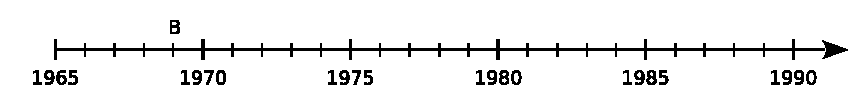
\includegraphics[width=\linewidth]{axe1965-1990}

Ce nombre est associé à un événement historique important. Lequel ?
Décalque cette demi-droite et place le point $N$ associé au nombre qui correspond à l'année de la chute du mur de Berlin.

Le nombre associé à un point sur une demi-droite graduée est l'\textbf{abscisse} de ce point.

\end{partie}

\begin{partie}[Des partages de plus en plus petits]
\begin{enumerate}
 \item Reproduis et complète la demi-droite graduée ci-dessous. \label{NbEntDec_Acti1Qa}
 
 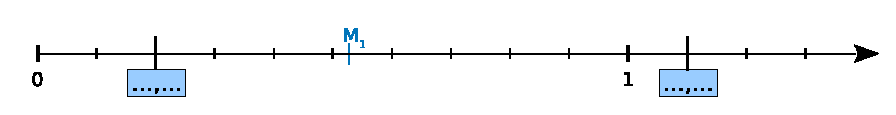
\includegraphics[width=\linewidth]{axe0-1}
 
 \item Détermine les abscisses des points $S$, $P$, $R$, $V$, $T$ et $U$ repérés en noir sur les demi-droites graduées ci-dessous.\label{NbEntDec_Acti1Qb}
 
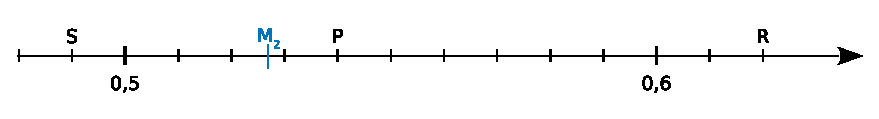
\includegraphics[width=\linewidth]{axe05-06}

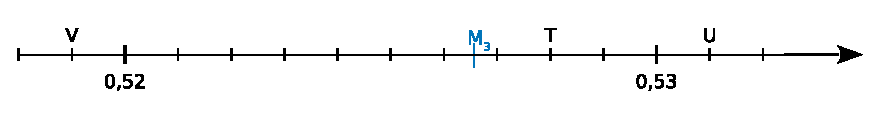
\includegraphics[width=\linewidth]{axe052-053}
 
 \item Sur une demi-droite, graduée judicieusement, place précisément les points $X$ et $Y$ d'abscisses respectives $0,526\,5$ et $0,527\,1$.
 \item Donne un \textbf{encadrement}, le plus précis possible, de l'abscisse des points $M_1$, $M_2$ et $M_3$ repérés en bleu sur les demi-droites graduées des questions \ref{NbEntDec_Acti1Qa} et \ref{NbEntDec_Acti1Qb}.
 \end{enumerate}
\end{partie}

\end{activite}


%%%%%%%%%%%%%%%%%%%%%%%%%%%%%%%%%%%%%%%%%%%%%%%%%%%%%%%%%%%%%%%%%%%%%%%%


\begin{activite}[L'écriture décimale]
\begin{enumerate}
 \item 349,785 est un nombre noté en écriture décimale. Dans ce nombre, quel est le chiffre représentant les unités ? Que désigne le chiffre 7 ? Et le chiffre 8 ?
 \item Le nombre 123,409 peut se lire « 123 virgule 409 ». Donne une autre lecture possible en utilisant les mots unités, dixièmes, centièmes et millièmes.
Que représente chacun des chiffres de ce nombre ? 4 est-il le chiffre des centaines ?
 \item Combien de centièmes y a-t-il dans un  dixième ? Dans une  unité ?
Combien de millièmes y a-t-il dans un centième ? Dans un dixième ? Dans une unité ?
 \item Combien de centièmes y a-t-il dans 7 unités 4 dixièmes ? Et dans 25 unités 8 dixièmes et 7 centièmes ?
 \end{enumerate}
\end{activite}


%%%%%%%%%%%%%%%%%%%%%%%%%%%%%%%%%%%%%%%%%%%%%%%%%%%%%%%%%%%%%%%%%%%%%%%%


\begin{activite}[Comparer, ranger et intercaler]

\begin{partie}[Comparer et ranger]
\begin{enumerate}
 \item Lequel des deux nombres 0,85 et 1,2 est le plus proche de 1 ? Quel est le nombre le plus proche de $12 : 11,9$ ou 12,08 ? Justifie avec soin tes réponses.
 \item Range les nombres de chaque liste dans l'ordre \textbf{croissant} (c'est-à-dire du plus petit au plus grand).
 	\begin{itemize}
	\item 1\,250 ; 1\,025 ; 125 ; 15\,200 ; 1\,520 ; 5\,120 ; 12\,500 ; 10\,520
	\item $10 + 0,5 + 0,06$ ; $7 + 0,5$ ; $10 + 0,06$ ; $7 + 0,05$ ; $10 + 0,6$ et $7 + 0,04 + 0,006$
	 \end{itemize}
 \item On a représenté ci-dessous une partie d'une demi-droite graduée.
 
 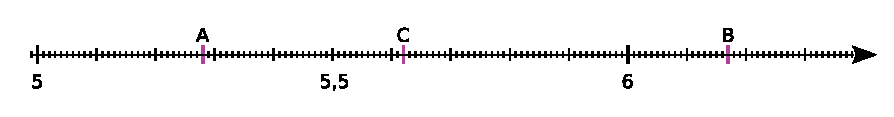
\includegraphics[width=\linewidth]{axe5A-6B}

Quelles sont les abscisses des points $A$, $B$ et $C$ ?

\vspace{0.75em}

Reproduis sur du papier millimétré cette portion de demi-droite et place les points $D$, $E$, $F$ et $G$ d'abscisses respectives 5,4 ; 6,22 ; 5,9 et 5,49.
Range alors les abscisses des points $A$, $B$, $C$, $D$, $E$, $F$ et $G$ dans l'ordre \textbf{décroissant}.
 \item À l'aide des questions précédentes et de tes connaissances, explique pourquoi les raisonnements d'élèves suivants ne sont pas justes et donne les raisons qui ont pu motiver leurs erreurs.
	\begin{itemize}
	\item \emph{« 24,5 < 6,08 car 245 < 608. »}
	\item \emph{« 19,85 < 12,96 car 0,85 < 0,96. »}
	\item \emph{« 6,012 > 6,35 car, à \textbf{partie entière} égale, le plus grand nombre est celui qui a le plus de chiffres après la virgule. »}
	\item \emph{« 5,24 > 5,8 car les parties entières sont égales et 24 > 8. »}
	\item \emph{« 14,3 < 14,30 car les parties entières sont égales et 3 < 30. »}
	\item \emph{« 103,6020 = 13,62 car les zéros ne servent à rien. »}
	\item \emph{« 16,295 < 16,38 car les parties entières sont égales et 16,295 a plus de chiffres après la virgule que 16,38. »}
	 \end{itemize}
 \end{enumerate}
\end{partie}

\begin{partie}[Intercaler]
\begin{enumerate}
 \item Quel est le nombre entier qui suit 128 ? Est-il possible de répondre à cette question si l'on remplace entier par décimal ?
Mêmes questions si on remplace 128 par 5,4.
 \item Est-il possible de trouver un nombre entier compris entre 1\,025 et 1\,026 ? Si oui, donne un exemple.
Même question en remplaçant « nombre entier » par « nombre décimal ».
 \item Est-il possible de trouver un nombre décimal compris entre 12,88 et 12,89 ? Et entre 8,975 et 8,976 ?
 \item À ton avis, est-il toujours possible de trouver plusieurs nombres décimaux compris entre deux nombres décimaux ?
 \end{enumerate}
\end{partie}

\end{activite}


%%%%%%%%%%%%%%%%%%%%%%%%%%%%%%%%%%%%%%%%%%%%%%%%%%%%%%%%%%%%%%%%%%%%%%%%

\begin{activite}[Multiplication et division par 10 ; 100 ; 1000 \ldots]

\begin{partie}[Multiplication par 10 ; 100 ; 1000 \ldots]
Le nombre 924,65 est égal à 9 centaines plus 2 dizaines plus 4 unités plus 6 dixièmes plus 5 centièmes.
\begin{enumerate}
 \item On veut multiplier par 10 le nombre suivant : 7 centaines plus 8 dizaines plus 3 unités plus 5 dixièmes plus 4 centièmes. Écris le résultat sous la même forme puis déduis-en une égalité en écriture décimale. \label{NbEntDec_Acti4Qa}
 \item Écris le nombre 15,034 comme dans la question \ref{NbEntDec_Acti4Qa}. Multiplie‑le par 1\,000 en t'inspirant de la question précédente.
 \item Donne une règle permettant de multiplier un nombre décimal par 10, 100 ou 1\,000. Que devient cette règle dans le cas d'un nombre entier ?
 \end{enumerate}
\end{partie}

\begin{partie}[Division par 10 ; 100 ; 1000 \ldots]
\begin{enumerate}
 \item En t'inspirant de la méthode précédente, divise par 10 le nombre 3 milliers plus 4 dizaines plus 6 unités plus 3 dixièmes plus 5 centièmes. Écris l'égalité en écriture décimale. \label{NbEntDec_Acti4Qa_2}
 \item Écris le nombre 73,305 comme dans la question \ref{NbEntDec_Acti4Qa_2} puis divise‑le par 1\,000.
 \item Donne une règle permettant de diviser un nombre décimal par 10, 100 ou 1\,000.
 \end{enumerate}
\end{partie}

\end{activite}


%%%%%%%%%%%%%%%%%%%%%%%%%%%%%%%%%%%%%%%%%%%%%%%%%%%%%%%%%%%%%%%%%%%%%%%%

\begin{activite}[Techniques opératoires]

\begin{partie}[Addition et soustraction de nombres décimaux]
\begin{enumerate}
 \item Pose et effectue l'opération $123,67 + 2,655$. Explique la méthode.
 \item Domitille et Virgile ont effectué cette opération et voilà ce qu'ils ont trouvé :\\[0.5em]
 
 \begin{minipage}[t]{.44\linewidth} 
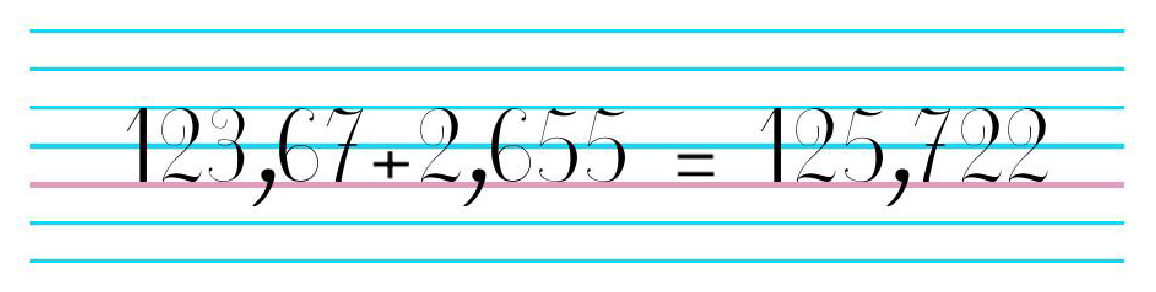
\includegraphics[width=5.5cm]{rep_domitille}
 \end{minipage}\hfill%
 \begin{minipage}[t]{.56\linewidth}
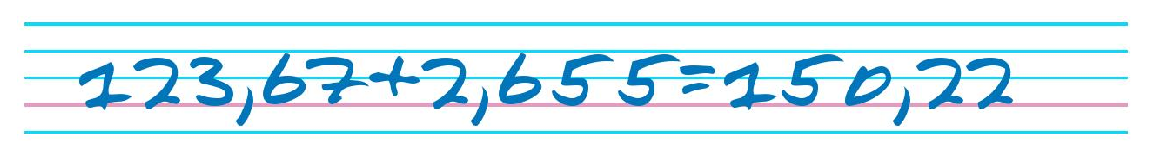
\includegraphics[width=7.5cm]{rep_virgile}
 \end{minipage}\\
  \begin{minipage}[t]{.44\linewidth} 
\begin{center} Réponse de Domitille \end{center}
 \end{minipage}\hfill%
 \begin{minipage}[t]{.56\linewidth}
\begin{center} Réponse de Virgile \end{center}
 \end{minipage}\\
 
 Que penses‑tu de leurs résultats ? Explique leurs éventuelles erreurs.
 \item Ambre était absente le jour où la maîtresse a expliqué comment on soustrait des nombres décimaux. Écris un texte le lui expliquant, donne un exemple.
 \end{enumerate}
\end{partie}

\begin{partie}[Multiplication d'un nombre décimal par un nombre entier]
\begin{enumerate}
 \item Pose et effectue l'opération $123,7 + 123,7 + 123,7 + 123,7$.
 \item Pose et effectue l'opération $123,7 \cdot 4$. Compare les deux opérations.
 \item Pose et effectue l'opération $52,8 \cdot 6$.
 \item Lucas a noté une série d'opérations pour calculer $52,8 \cdot 6$ : \\[-1em]
 
 $0,8 \cdot 6 = 4,8$ \hfill $2 \cdot 6 = 12$ \hfill $50 \cdot 6 = 300$ \hfill $300 + 12 + 4,8 = 316,8$ \\[-1em]
 
 Que penses‑tu de cette méthode ?
 \item Effectue l'opération $763,6 \cdot 3$ en utilisant la méthode de Lucas puis pose‑la pour vérifier ton résultat.
 \item Adapte cette méthode pour effectuer l'opération $1,34 \cdot 18$. Pose ensuite l'opération pour vérifier ton résultat.
 \end{enumerate}
\end{partie}

\end{activite}


%%%%%%%%%%%%%%%%%%%%%%%%%%%%%%%%%%%%%%%%%%%%%%%%%%%%%%%%%%%%%%%%%%%%%%%%



\begin{activite}[Vérifier un résultat]

\begin{enumerate}
 \item Sans poser aucune opération et sans utiliser de calculatrice, associe chaque calcul de gauche à un résultat de droite. \\[0.5em]
 
\begin{minipage}[t]{0.48\linewidth}
\begin{center}
\begin{ttableau}{0.7\linewidth}{1}
\hline \rowcolor{B3} \textbf{a.} $\quad 56 \cdot 123$ \\
\hline \rowcolor{G3} \textbf{b.} $\quad 12,35 + 1,68$ \\
\hline \rowcolor{B3} \textbf{c.} $\quad 1\,073 : 200$ \\
\hline \rowcolor{G3} \textbf{d.} $\quad 0,255 + 0,728$ \\
\hline \rowcolor{B3} \textbf{e.} $\quad 0,255 \cdot 0,728$ \\
\hline \rowcolor{G3} \textbf{f.} $\quad 13,23 : 5$ \\
\hline \rowcolor{B3} \textbf{g.} $\quad 520 \cdot 36$ \\
\hline \rowcolor{G3} \textbf{h.} $\quad 428 + 537$ \\
\hline \rowcolor{B3} \textbf{i.} $\quad 1,2 \cdot 2,4$ \\
\hline \rowcolor{G3} \textbf{j.} $\quad 18 \cdot 29$ \\
\hline
\end{ttableau}
\end{center}
\end{minipage} \hfill%
\begin{minipage}[t]{0.48\linewidth}
\begin{center}
\renewcommand*\tabularxcolumn[1]{>{\centering\arraybackslash}m{#1}}
\begin{ttableau}{0.6\linewidth}{1}
\hline \rowcolor{H3} 5,365 \\
\hline \rowcolor{J3} 2,88 \\
\hline \rowcolor{H3} 6\,888 \\
\hline \rowcolor{J3} 0,983 \\
\hline \rowcolor{H3} 2,646 \\
\hline \rowcolor{J3} 965 \\
\hline \rowcolor{H3} 522 \\
\hline \rowcolor{J3} 14,03 \\
\hline \rowcolor{H3} 18\,720 \\
\hline \rowcolor{J3} 0,185\,64 \\
\hline
\end{ttableau} 
\end{center}
 \end{minipage} \\
 
 \item Explique le plus précisément possible la manière dont tu as trouvé les résultats.\label{NbEntDec_Acti6Q2}
 \item Maverick a effectué des calculs ci-dessous. Détermine quels résultats sont forcément faux en utilisant les méthodes décrites à la question \ref{NbEntDec_Acti6Q2}.\\[1em]
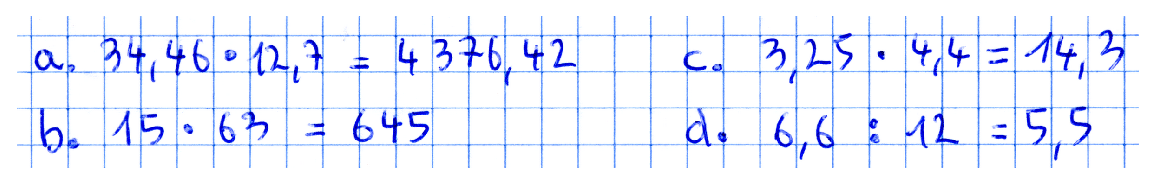
\includegraphics[width=\linewidth]{calcul_Maverick}

 \end{enumerate}
 
 \end{activite}


%%%%%%%%%%%%%%%%%%%%%%%%%%%%%%%%%%%%%%%%%%%%%%%%%%%%%%%%%%%%%%%%%%%%%%%%




\cours
\section{Le système décimal}

% remarque : pour qu'un mot se retrouve dans le lexique : \MotDefinition{asymptote horizontale}{} 

Les règles et conventions qui permettent d'écrire et de lire les nombres forment ce qu'on appelle un \textbf{système de numération}. Nous utilisons le système décimal, de base dix.

\begin{aconnaitre}
Pour écrire les chiffres dans le système décimal, il nous faut dix symboles, appelés des \emph{chiffres}. Ces chiffres sont :
\[ 0\,;\,1\,;\,2\,;\,3\,;\,4\,;\,5\,;\,6\,;\,7\,;\,8\,;\,9  \]
Il arrive parfois qu'on confonde \textbf{\MotDefinition{chiffre}{}} et \textbf{\MotDefinition{nombre}{}}. On peut faire l'analogie avec l'écriture d'une langue en affirmant que les \textbf{\textcolor{H1}{chiffres}} sont des \textbf{\textcolor{H1}{lettres}} et que les \textbf{\textcolor{H1}{nombres}} sont des \textbf{\textcolor{H1}{mots}}. Ainsi, 13 est un nombre qui s'écrit avec les chiffres 1 et 3.
\end{aconnaitre}

\newpage

\begin{methode*1}[Écriture et lecture des nombres en base 10]

L'\textbf{\textcolor{C2}{écriture décimale}} d'un nombre comporte deux parties, séparées par une virgule :

\hspace{2em}\textbullet\hspace{.25em} la partie entière, à gauche de la virgule ;

\hspace{2em}\textbullet\hspace{.25em} la partie décimale, à droite de la virgule.



Un nombre entier est caractérisé par le fait qu'il n'a pas de partie décimale (on omet alors la virgule).

\vspace{2em}

\begin{ttableau}{\linewidth}{18}
\hline
\multicolumn{3}{|c|}{milliards} & \multicolumn{3}{c|}{millions} & \multicolumn{3}{c|}{mille} & \multicolumn{3}{c|}{unités} & \multirow{2}{*}{\rotatebox{90}{dixièmes\phantom{xxx}}} & \multirow{2}{*}{\rotatebox{90}{centièmes\phantom{xxx}}} & \multirow{2}{*}{\rotatebox{90}{millièmes\phantom{xxx}}} & \multirow{2}{*}{\rotatebox{90}{dix-millièmes\phantom{xxx}}} & \multirow{2}{*}{\rotatebox{90}{centi-millièmes\phantom{xxx}}} & \multirow{2}{*}{\rotatebox{90}{millionièmes\phantom{xxx}}} \\ \cline{1-12}
\rotatebox{90}{centaines de ... } & \rotatebox{90}{dizaines de ...} & \rotatebox{90}{unités de ...} &
\rotatebox{90}{centaines de ... } & \rotatebox{90}{dizaines de ...} & \rotatebox{90}{unités de ...} &
\rotatebox{90}{centaines de ... } & \rotatebox{90}{dizaines de ...} & \rotatebox{90}{unités de ...} &
\rotatebox{90}{centaines de ... } & \rotatebox{90}{dizaines de ...} & \rotatebox{90}{unités de ...} & & & & & & \\ \hline
& & & & & & & & & & & & & & & & & \\ \hline
& & & & & 3 & 0 & 2 & 7 & 4 & 6 & 2 & 0 & 0 & 0 & 0 & 0 & 0 \\ \hline
& & & & & & & & & & 1 & 0 & 0 & 1 & & & & \\ \hline
& & & & & & & & & & & 0 & 0 & 3 & 7 & & & \\ \hline
& 2 & 0 & 0 & 0 & 0 & 0 & 4 & 2 & 0 & 0 & 0 & & & & & & \\ \hline
\end{ttableau}


\begin{exemple*1}
Le premier nombre figurant dans le tableau s'écrit 3\,027\,462.

Il se lit "trois millions vingt-sept mille quatre cent soixante-deux".

C'est un nombre entier.
\end{exemple*1}

\begin{exemple*1}
Le  deuxième nombre figurant dans le tableau s’écrit 10,01.

Il se lit "dix virgule zéro un".

Ce n’est pas un nombre entier.
\end{exemple*1}

\begin{exemple*1}
Le troisième nombre figurant dans le tableau s’écrit 0,037.

Il se lit "zéro virgule zéro trente-sept" ou "trente-sept millièmes".

Ce n’est pas un nombre entier.
\end{exemple*1}

\begin{exemple*1}
Le quatrième nombre figurant dans le tableau s’écrit 20\,000\,042\,000.

Il se lit "vingt milliards quarante-deux mille".

C’est un nombre entier.
\end{exemple*1}

\exercice 

Donne une écriture décimale du nombre cinquante-trois millions quatre cent vingt-sept mille huit cent dix-neuf virgule zéro zéro cinq cent soixante-et-un.
%\correction

\end{methode*1}

%%%%%%%%%%%%%%%%%%%%%%%%%%%%%%%%%%%%%%%%%%%%%%%%%%%%%%%%%%%%%%%%%%%%%%%%%%%

\begin{methode*1}[Repérer sur une demi-droite graduée]

\begin{aconnaitre}
Sur une demi-droite graduée, un point est repéré par un nombre appelé son \textbf{\MotDefinition{abscisse}{}}.
\end{aconnaitre}

\begin{exemple*1}

\vspace{0.5cm}

 \begin{minipage}[c]{.46\textwidth}
 Donne l'abscisse des points $A$ et $B$ puis place le point $C$ d'abscisse 4,3.
  \end{minipage}\hfill%
 \begin{minipage}[c]{.46\textwidth} 
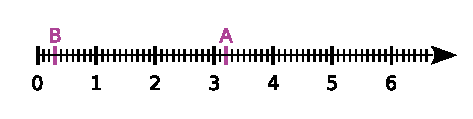
\includegraphics[width=5.5cm]{axe0BA6}
 \end{minipage}\\

Une unité est divisée en dix parts égales, ce qui signifie qu'elle est partagée en dix dixièmes. Le point $A$ se trouve 2 dixièmes à la droite du 3, donc son abscisse est $3 + 0,2 = 3,2$. De la même façon, $B$ a pour abscisse $0 + 0,3 = 0,3$. \\

  \begin{minipage}[c]{.46\textwidth}
On note $A(3,2)$ et $B(0,3)$.\\
$C(4,3) : 4,3 = 4 + 0,3$\\
$C$ se place 3 dixièmes à la droite du 4.
  \end{minipage}\hfill%
 \begin{minipage}[c]{.46\textwidth} 
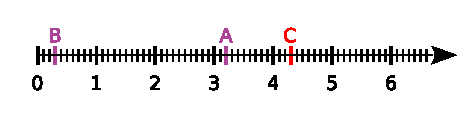
\includegraphics[width=5.5cm]{axe0BAC6}
 \end{minipage}\\

\end{exemple*1}

\exercice 

Sur une demi-droite graduée, place les points $M$ d'abscisse 2,7 et $N$ d'abscisse 5,2.
%\correction

\end{methode*1}

%%%%%%%%%%%%%%%%%%%%%%%%%%%%%%%%%%%%%%%%%%%%%%%%%%%%%%%%%%%%%%%%%%%%%%%%%%%
\begin{methode*1}[Encadrer]

\begin{aconnaitre}
\textbf{\MotDefinition{Encadrer}{}} un nombre, c'est trouver un nombre qui est plus petit que lui et un nombre qui est plus grand que lui. On écrit un encadrement avec les symboles $<$ ; $\leqslant$ ; $>$ et $\geqslant$. 
\end{aconnaitre}

\begin{exemple*1}
Encadrer 13,345 à l'unité puis au centième.\\[0.5em]
Pour encadrer à l'unité, on «coupe» le nombre 13,345 à l'unité et on obtient 13 qui est plus petit  que 13,345. Puis on ajoute \textbf{une unité}. On obtient 14 qui est plus grand que 13,345. On écrit alors : $13 < 13,345 < 14$. \\[1em]
Pour encadrer au centième, on «coupe» le nombre 13,345 au centième et on obtient 13,34 qui est plus petit que 13,345. Puis on ajoute \textbf{un centième}. On obtient 13,35 qui est plus grand que 13,345. On écrit alors : $13,34 < 13,345 < 13,35$.
\end{exemple*1}

\exercice

Encadrer les nombres 237,48 et 43,923\,5 à la dizaine puis au centième.
%\correction

\end{methode*1}

%%%%%%%%%%%%%%%%%%%%%%%%%%%%%%%%%%%%%%%%%%%%%%%%%%%%%%%%%%%%%%%%%%%%%%%%%%

\begin{methode*1}[Arrondir]

\begin{aconnaitre}
\textbf{\MotDefinition{Arrondir}{}} un nombre, c’est le remplacer par le nombre le plus proche à la précision désirée. Pour cela, on choisit le dernier chiffre à conserver puis :
\begin{itemize}
 \item on conserve ce chiffre si le suivant est 0, 1, 2, 3 ou 4 ;
 \item on augmente de 1 ce chiffre si le suivant est 5, 6, 7, 8, ou 9.
 \end{itemize}
\end{aconnaitre}

\exercice

%\correction

\end{methode*1}

%%%%%%%%%%%%%%%%%%%%%%%%%%%%%%%%%%%%%%%%%%%%%%%%%%%%%%%%%%%%%%%%%%%%%%%%%%

\section{Multiplier ou diviser}

\begin{methode*1}[Multiplier ou diviser un nombre décimal par 10 ; 100 ; 1\,000 \ldots]

\begin{aconnaitre}
\textbf{Multiplier} un nombre décimal par \textcolor{A1}{\textbf{10}}, \textcolor{B1}{\textbf{100}} ou \textcolor{J1}{\textbf{1\,000}} revient à déplacer chacun de ses chiffres vers \textbf{la gauche} de \textcolor{A1}{\textbf{1}}, \textcolor{B1}{\textbf{2}} ou \textcolor{J1}{\textbf{3}} rangs pour lui donner une valeur \textcolor{A1}{\textbf{10}}, \textcolor{B1}{\textbf{100}} ou \textcolor{J1}{\textbf{1\,000}} fois plus grande.
\textbf{Diviser} un nombre décimal par \textcolor{A1}{\textbf{10}}, \textcolor{B1}{\textbf{100}} ou \textcolor{J1}{\textbf{1\,000}} revient à déplacer chacun de ses chiffres vers \textbf{la droite} de \textcolor{A1}{\textbf{1}}, \textcolor{B1}{\textbf{2}} ou \textcolor{J1}{\textbf{3}} rangs pour lui donner une valeur  \textcolor{A1}{\textbf{10}}, \textcolor{B1}{\textbf{100}} ou \textcolor{J1}{\textbf{1\,000}} fois plus petite.
\end{aconnaitre}

\begin{remarque}
On devra parfois ajouter des zéros dans l'écriture.
\end{remarque}

\begin{exemple*1}
Effectue les calculs $6,5:100$ et $0,47 \cdot 1\,000$.\\[1em] 

\begin{minipage}{.4\linewidth}
\begin{ttableau}{.8\linewidth}{4}
\hline
 \rotatebox{90}{unités} & \rotatebox{90}{dixièmes} & \rotatebox{90}{centièmes\phantom{x}} & \rotatebox{90}{millièmes} \\ \hline
 \textcolor{B1}{\textbf{6}} , & \textcolor{B1}{\textbf{5}} & & \\ \hline
 $0\,,$ & 0 & \textcolor{B1}{\textbf{6}} & \textcolor{B1}{\textbf{5}} \\ \hline
\end{ttableau}
\end{minipage}\hfill%
%
\begin{minipage}{.55\linewidth}
Pour diviser 6,5 par \textcolor{B1}{\textbf{100}}, on déplace chacun de ses chiffres vers la droite de \textcolor{B1}{\textbf{2}} rangs et on ajoute les zéros nécessaires. 

On obtient $6,5:100 = 0,065$.

\end{minipage}
%

\vspace{2em}

%
\begin{minipage}{.4\linewidth}
\begin{ttableau}{\linewidth}{5}
\hline
\rotatebox{90}{centaines} & \rotatebox{90}{dixaines} & \rotatebox{90}{unités} & \rotatebox{90}{dixièmes} & \rotatebox{90}{centièmes\phantom{x}} \\ \hline
 & & 0 , & \textcolor{J1}{\textbf{4}} & \textcolor{J1}{\textbf{7}} \\ \hline
 \textcolor{J1}{\textbf{4}} & \textcolor{J1}{\textbf{7}} & 0 & &\\ \hline
\end{ttableau}
\end{minipage}\hfill%
%
\begin{minipage}{.55\linewidth}
Pour multiplier 0,47 par \textcolor{J1}{\textbf{1\,000}}, on déplace chacun de ses chiffres vers la gauche de \textcolor{J1}{\textbf{3}} rangs et on ajoute les zéros nécessaires. 

On obtient $0,47 \cdot 1\,000 = 470$. 
\end{minipage}
\end{exemple*1}

\exercice

Effectue : 
\begin{colenumerate}{4}
 \item $3,6 \cdot 100$ ;
 \item $870 \cdot 1\,000$ ;
 \item $63 : 10$ ;
 \item $87\,654 : 100$.
 \end{colenumerate}
%\correction
 
\exercice

Convertis en cm :
\begin{colenumerate}{4}
 \item 4 dm ;
 \item 8,1 dam ;
 \item 3,5 mm ;
 \item 0,035 m.
 \end{colenumerate}
%\correction

\end{methode*1}

%%%%%%%%%%%%%%%%%%%%%%%%%%%%%%%%%%%%%%%%%%%%%%%%%%%%%%%%%%%%%%%%%%%%%%%%%%%

\begin{methode*1}[Multiplier ou diviser un nombre décimal par 0,1 ; 0,01 ; 0,001 \ldots]

\begin{aconnaitre}
\textbf{Multiplier} un nombre décimal par \textcolor{A1}{\textbf{0,1}}, \textcolor{B1}{\textbf{0,01}} ou \textcolor{J1}{\textbf{0,001}} revient à déplacer chacun de ses chiffres vers \textbf{la droite} de 1, 2 ou \textcolor{J1}{\textbf{3}} rangs pour lui donner une valeur 10, 100 ou \textcolor{J1}{\textbf{1\,000}} fois plus petite.
\textbf{Diviser} un nombre décimal par \textcolor{A1}{\textbf{0,1}}, \textcolor{B1}{\textbf{0,01}} ou \textcolor{J1}{\textbf{0,001}} revient à déplacer chacun de ses chiffres vers \textbf{la gauche} de \textcolor{A1}{\textbf{1}}, \textcolor{B1}{\textbf{2}} ou \textcolor{J1}{\textbf{3}} rangs pour lui donner une valeur \textcolor{A1}{\textbf{10}}, \textcolor{B1}{\textbf{100}} ou \textcolor{J1}{\textbf{1\,000}} fois plus grande.
\end{aconnaitre}

\begin{remarque}
On devra parfois ajouter des zéros dans l'écriture.
\end{remarque}

\begin{exemple*1}
Effectue les calculs $2,5 \times 0,01$ et $0,65 \div 0,001$.\\[1em]

\begin{minipage}{.4\linewidth}
\begin{ttableau}{.8\linewidth}{4}
\hline
 \rotatebox{90}{unités} & \rotatebox{90}{dixièmes} & \rotatebox{90}{centièmes\phantom{x}} & \rotatebox{90}{millièmes} \\ \hline
 \textcolor{B1}{\textbf{2}} , & \textcolor{B1}{\textbf{5}} & & \\ \hline
 $0\,,$ & 0 & \textcolor{B1}{\textbf{2}} & \textcolor{B1}{\textbf{5}} \\ \hline
\end{ttableau}
\end{minipage}\hfill%
%
\begin{minipage}{.55\linewidth}
Pour multiplier 2,5 par \textcolor{B1}{\textbf{0,01}}, on déplace chacun de ses chiffres vers la droite de \textcolor{B1}{\textbf{2}} rangs et on ajoute les zéros nécessaires. 

On obtient $2,5 \times 0,01 = 0,025$.
\end{minipage}
%

\vspace{2em}

%
\begin{minipage}{.4\linewidth}
\begin{ttableau}{\linewidth}{5}
\hline
\rotatebox{90}{centaines} & \rotatebox{90}{dixaines} & \rotatebox{90}{unités} & \rotatebox{90}{dixièmes} & \rotatebox{90}{centièmes\phantom{x}} \\ \hline
 & & 0 , & \textcolor{J1}{\textbf{6}} & \textcolor{J1}{\textbf{5}} \\ \hline
 \textcolor{J1}{\textbf{6}} & \textcolor{J1}{\textbf{5}} & 0 & &\\ \hline
\end{ttableau}
\end{minipage}\hfill%
%
\begin{minipage}{.55\linewidth}
Pour diviser 0,65 par \textcolor{J1}{\textbf{0,001}}, on déplace chacun de ses chiffres vers la gauche de \textcolor{J1}{\textbf{3}} rangs et on ajoute les zéros nécessaires. 

On obtient $0,65 \div 0,001 = 650$.
\end{minipage}
\end{exemple*1}


\exercice

Effectuer :
\begin{colenumerate}{4}
 \item $5,45 \cdot 0,1$ ;
 \item $854 \cdot 0,001$ ;
 \item $63 \div 0,1$ ;
 \item $87,54 \div 0,01$.
 \end{colenumerate}
%\correction

\end{methode*1}

%%%%%%%%%%%%%%%%%%%%%%%%%%%%%%%%%%%%%%%%%%%%%%%%%%%%%%%%%%%%%%%%%%%%%%%%%%%

\begin{methode*1}[Multiplier deux nombres décimaux]

\begin{exemple*1}

Effectue la multiplication de 2,34 par 1,2.\\[1em]

On pose l'opération comme s'il s'agissait de nombres entiers. 

On effectue la multiplication de 234 par 12 sans tenir compte des virgules.

\begin{minipage}{.6\linewidth}
\begin{tabular}{rrrrcrrrr}
& 2, & 3 & 4 & $\xrightarrow{\times \text{\textcolor{B1}{\textbf{100}}}}$ & & 2 & 3 & 4 \\
$\cdot$ & & 1, & 2 & $\xrightarrow{\times \text{\textcolor{A1}{\textbf{10}}}}$ & $\cdot$ & & 1 & 2 \\ \cline{1-4} \cline{6-9}
& & & & & & 4 & 6 & 8 \\
& & & & & 2 & 3 & 4 & . \\ \cline{1-4} \cline{6-9}
2, & 8 & 0 & 8 & $\xleftarrow{\,:\,\text{\textcolor{J1}{\textbf{1\,000}}}}$ & 2 & 8 & 0 & 8 \\
\end{tabular}
\end{minipage}\hfill%
%
\begin{minipage}{.37\linewidth}
234 est \textcolor{B1}{\textbf{100}} fois plus grand que 2,34 et 12 est \textcolor{A1}{\textbf{10}} fois plus grand que 1,2. Le produit $2,34 \cdot 1,2$ est donc \textcolor{J1}{\textbf{1\,000}} fois plus petit que 2\,808. Pour obtenir le résultat, on effectue donc $2\,808 : 1\,000$.\\[0.75em]
\end{minipage}
Finalement $2,34 \cdot 1,2 = 2,808$.
\end{exemple*1}

\exercice
Sachant que $168 \cdot 32 = 5\,376$, détermine les produits (sans aucun calcul) :
\begin{colenumerate}{4}
 \item $168 \cdot 3,2$ ;
 \item $16,8 \cdot 0,32$ ;
 \item $1\,680 \cdot 3,2$ ;
 \item $1,68 \cdot 32$.
\end{colenumerate}
%\correction

\exercice

Pose et effectue les opérations :
\begin{colenumerate}{4}
 \item $68,7 \cdot 39$ ;
 \item $123 \cdot 6,3$ ;
 \item $1,3 \cdot 0,7$ ;
 \item $54,6 \cdot 8,25$.
\end{colenumerate}
%\correction

\end{methode*1}

%%%%%%%%%%%%%%%%%%%%%%%%%%%%%%%%%%%%%%%%%%%%%%%%%%%%%%%%%%%%%%%%%%%%%%%%%%%    

\begin{methode*1}[Diviser un nombre décimal par un nombre entier]

\begin{exemple*1}
Effectue la division de 75,8 par 4.\\[0.5em]

\begin{minipage}[c]{.26\textwidth}
\vspace{0em}
\begin{center}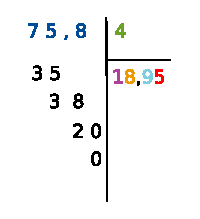
\includegraphics[width=3cm]{div758-4} \end{center}

\end{minipage}\hfill% 
\begin{minipage}[c]{.66\textwidth}

On commence par diviser la partie entière. On partage \textcolor{A1}{7} dizaines en \textcolor{H1}{4} ; le quotient comportera \textcolor{C1}{1} dizaine.\\[0.75em]
Il reste 3 dizaines. Avec les \textcolor{A1}{5} unités en plus, cela fait 35 unités à partager en \textcolor{H1}{4} ; le quotient comportera \textcolor{J1}{8} unités. \\[0.75em]
Il reste 3 unités soit 30 dixièmes. Avec les \textcolor{A1}{8} dixièmes en plus, cela fait 38 dixièmes à partager en \textcolor{H1}{4} ; le quotient comportera \textcolor{A3}{9} dixièmes. On doit donc écrire la virgule dans le quotient.\\[0.75em]
Il reste 2 dixièmes soit 20 centièmes (on a ajouté un zéro) à partager en \textcolor{H1}{4} ; le quotient comportera donc \textcolor{B2}{5} centièmes.\\[0.75em]
Ainsi $\textcolor{A1}{75,8} : \textcolor{H1}{4} = \textcolor{C1}{1}\textcolor{J1}{8},\textcolor{A3}{9}\textcolor{B2}{5}$.
\end{minipage}

\end{exemple*1}

\exercice

Calcule la valeur exacte ou une valeur arrondie au centième des quotients :
\begin{colenumerate}{4}
 \item $10 : 7$ ;
 \item $24,96 : 8$ ;
 \item $5,2 : 6$ ;
 \item $145,2 : 3$.
 \end{colenumerate}
%\correction

\end{methode*1}

%%%%%%%%%%%%%%%%%%%%%%%%%%%%%%%%%%%%%%%%%%%%%%%%%%%%%%%%%%%%%%%%%%%%%%%%%%%

\begin{methode*1}[Diviser un nombre décimal par un nombre décimal]

\begin{aconnaitre}
Le quotient de deux nombres \textbf{ne change pas} si on les multiplie (le dividende et le diviseur) par un même nombre non nul.
\end{aconnaitre}

\begin{exemple*1}
Effectue la division de 32,4 par 2,25.\\[1em]
On commence par rendre entier le diviseur en le multipliant par 100 : $2,25 \cdot 100 = 225$. On multiplie le dividende par le même nombre : $32,4 \cdot 100 = 3\,240$. On effectue la division de 3\,240  par 226, soit $3\,240 : 225 = 14,4$. On obtient ainsi le résultat de la division :

$32,4 : 2,25 = 14,4$. 
\end{exemple*1}

\exercice

Calcule la valeur exacte ou une valeur arrondie au centième des quotients :
\begin{colenumerate}{4}
 \item $4 : 6,37$ ;
 \item $13,4 : 2,45$ ;
 \item $5,87 : 2,3$ ;
 \item $0,84 : 0,12$.
 \end{colenumerate}
%\correction

\end{methode*1}

%%%%%%%%%%%%%%%%%%%%%%%%%%%%%%%%%%%%%%%%%%%%%%%%%%%%%%%%%%%%%%%%%%%%%%%%%%%        

\section{Opérations sur les durées}


%%%%%%%

\begin{methode*1}[Conversion en minutes ou en secondes]

\begin{exemple*1}

\begin{enumerate}
\item Combien y a-t-il de minutes dans 5 h 27 min ?

\begin{tabular}{ll} 
\textcolor{bleu}{\textbf{5 h}} $=$ \textcolor{bleu}{\textbf{5}} $\times$ 60 min $=$ \textcolor{bleu}{\textbf{300 min}}  & $\rightarrow$ Convertir les heures en minutes. \\
\textcolor{bleu}{\textbf{5 h}} \textcolor{vert}{\textbf{27 min}} $=$ \textcolor{bleu}{\textbf{300 min}} $+$ \textcolor{vert}{\textbf{27 min}} $=$ 327 min & $\rightarrow$ Terminer le calcul.\\
%\phantom{2 h 47 min 53 s $=$ 7\,200 s $+$ 2\,820 s $+$ 53} & \\ % phantom pour alignement avec tableau ci-dessous
\end{tabular} 

\vspace{2em}\item Combien y a-t-il de secondes dans 2 h 47 min 53 s ?

\begin{tabular}{ll} 
\textcolor{bleu}{\textbf{2 h}} $=$ \textcolor{bleu}{\textbf{2}} $\times$ 3\,600 s $=$ \textcolor{bleu}{\textbf{7\,200 s}} & $\rightarrow$ Convertir les heures en secondes. \\
\textcolor{vert}{\textbf{47 min}} $=$ \textcolor{vert}{\textbf{47}} $\times$ 60 s $=$ \textcolor{vert}{\textbf{2\,820}} s & $\rightarrow$ Convertir les minutes en secondes. \\
\textcolor{bleu}{\textbf{2 h}} \textcolor{vert}{\textbf{47 min}} 53 s $=$ \textcolor{bleu}{\textbf{7\,200 s}} $+$ \textcolor{vert}{\textbf{2\,820}} s $+$ 53 s  \\
\phantom{2 h 47 min 53 si}$=$ 10\,073 s & $\rightarrow$ Terminer le calcul. \\
\end{tabular}

\end{enumerate}
 
\end{exemple*1}

\exercice

\end{methode*1}



%%%%%%%


\begin{methode*1}[Conversion en heures, minutes et secondes]

\begin{exemple*1}
Combien y a-t-il d'heures, minutes et secondes dans 41\,000 s ? \\[1em]
\begin{minipage}[t]{.46\textwidth}
On convertit les secondes en minutes et secondes en posant la division de 41\,000 par 60 :

\begin{center}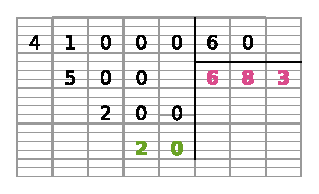
\includegraphics[width=4.6cm]{41000div60} \end{center}

On a donc 41\,000 s $=$ \textcolor{rose}{\textbf{683 min}} \textcolor{vert}{\textbf{20 s}}.
\end{minipage}\hfill%
\begin{minipage}[t]{.46\textwidth}
On convertit alors les minutes en heures et minutes en effectuant la division euclidienne de 683 par 60 :

\begin{center}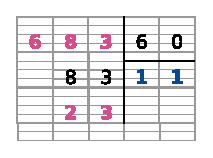
\includegraphics[width=2.9cm]{683div60} \end{center}
On a donc 41\,000 s $=$ \textcolor{bleu}{\textbf{11 h}} \textcolor{rose}{\textbf{23 min}} \textcolor{vert}{\textbf{20 s}}.
\end{minipage}


\end{exemple*1}

\exercice

\end{methode*1}

%%%%%%%%%%%%

\begin{methode*1}[Addition de durées]

\begin{exemple*1}
Un match dure 3 h 38 min et le suivant dure 2 h 49 min. Quelle est la durée totale de ces deux matchs ? \\[1em]
\begin{minipage}[t]{.34\textwidth}
On pose l'addition suivante :\\[0.2em]

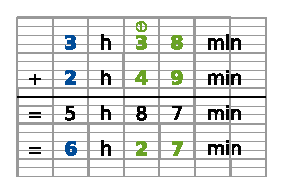
\includegraphics[width=\linewidth]{grille3h38}
\end{minipage}\hfill%
\begin{minipage}[t]{.60\textwidth}
On effectue deux additions indépendantes : 
\textcolor{vert}{\textbf{les minutes entre elles}} et \textcolor{bleu}{\textbf{les heures entre elles}}.\\[0.75em]
Mais le nombre de minutes obtenu est supérieur à 59. 
On va donc le convertir en heures et minutes sachant que 60 min $=$ 1 h. \\[0.75em]
La durée totale de ces deux matchs est donc de \textcolor{rose}{\textbf{6 h 27 min}}.
\end{minipage}

\end{exemple*1}

\exercice

Calcule :

3 h 05 min 13 s $+$ 56 min 48 s.

\vspace{1em}

1 h 46 min $+$ 2 h 37 min.

\end{methode*1}

%%%%%%%%%%%%

\begin{methode*1}[Soustraction de durées]

\begin{exemple*1}
Un film débute à 15 h 27 et finit à 18 h 14. Quelle est la durée de ce film ? \\[1em]

\begin{minipage}[t]{.34\textwidth}
On pose la soustraction suivante :\\[0.2em]

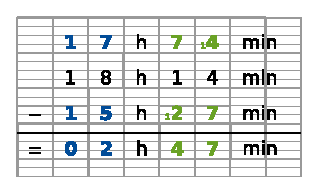
\includegraphics[width=\linewidth]{grille17h74}
\end{minipage}\hfill%
\begin{minipage}[t]{.60\textwidth}
On effectue deux soustractions indépendantes : 
\textcolor{vert}{\textbf{les minutes entre elles}} et \textcolor{bleu}{\textbf{les heures entre elles}}.\\[0.75em]
Mais on ne peut pas enlever 27 à 14. 
On va donc convertir 1 des 18 heures en 60 min. \\[0.75em]
Ce film dure donc \textcolor{rose}{\textbf{2 h 47 min}}.
\end{minipage}

\end{exemple*1}

\exercice

Calcule :

1 h 35 min 29 s $-$ 46 min 37 s.

\vspace{1em}

9 min 16 s $-$ 7 min 55 s.

%\correction

\end{methode*1}

\exercicesbase
\begin{colonne*exercice}
 \definecolor{fondTI}{HTML}{869286}


\serie{Les nombres entiers}

\begin{exercice}[Un peu de vocabulaire]
Recopie et complète les phrases suivantes afin de les rendre exactes :
\begin{enumerate}
 \item Un \ldots \ldots \ldots est composé de chiffres ;
 \item 9 est un \ldots \ldots \ldots composé d'un seul \ldots \ldots \ldots ;
 \item Le chiffre des centaines du nombre 2\,568 est \ldots \ldots ;
 \item 3 est le chiffre des \ldots \ldots \ldots du nombre 783 ;
 \item \ldots \ldots est le chiffre des milliers du nombre 120\,452 ;
 \item Le chiffre des \ldots \ldots \ldots du nombre 43 est 4.
\end{enumerate}
\end{exercice}


\begin{exercice}[« Chiffre des » ou « nombre de »]
\begin{enumerate}
 \item Recopie et complète les phrases suivantes afin de les rendre exactes :
 \begin{itemize}
  \item $127 = 12 \cdot \ldots + 7$:
  
  127 possède donc \ldots \ldots dizaines ;
  \item $841\,123 = 841 \cdot \ldots + \ldots \ldots$ :
  
  841\,123 possède donc 841 \ldots \ldots ;
  \item $3\,816 = \ldots \cdot 100 + \ldots \ldots$ :
  
  \ldots \ldots possède donc \ldots \ldots .
  \end{itemize}
 \item Dans le nombre entier 15, quel est le nombre d'unités ? Le chiffre des unités ?
 \item Combien y a-t-il de centaines dans 4\,125 ?
 \item Quel est le chiffre des dizaines dans le nombre entier 498 ? Et le nombre de dizaines ?
 \item Dans 25 dizaines, quel est le nombre d'unités ?
 \end{enumerate}
\end{exercice}


\begin{exercice}
Donne l'écriture en chiffres des nombres entiers suivants :
\begin{enumerate}
 \item $(9 \cdot 10) + 5$ ;
 \item $(7 \cdot 1\,000) + (5 \cdot 100) + (2 \cdot 10) + 8$ ;
 \item $(1 \cdot 10\,000) + (1 \cdot 100) + 1$ ;
 \item  $(3 \cdot 100\,000) + (7 \cdot 10\,000) + (4 \cdot 10) + 9$ ;
 \item  $(3 \cdot 100\,000) + (4 \cdot 100) + (7 \cdot 1\,000) + 9$.
 \end{enumerate}
\end{exercice}


\begin{exercice}
Écris en chiffres les nombres suivants :
\begin{enumerate}
 \item Sept mille huit cent douze ;
 \item Soixante-trois mille neuf cent cinquante ;
 \item Huit millions trois ;
 \item Septante-quatre milliards cent quatre ;
 \item Cent trente-six millions huit cent nonante-trois mille sept cent cinq.
 \end{enumerate}
\end{exercice}

%%%%%%%%%%%%%
\vspace{1em}%
%%%%%%%%%%%%%

\begin{exercice}
Classe les nombres suivants dans l'ordre décroissant (du plus grand au plus petit) :
\begin{colitemize}{2}
 \item 23\,100 ;
 \item Cent vingt-trois mille ;
 \item 1\,320 ;
 \item Mille cent vingt-trois.
 \end{colitemize}
\end{exercice}

%%%%%%%%%%%%%%%%%%%%%%%%%%%%%%%%%%%%%%%%%%%%%%%%%%%%%%%%%%%%%%%%%%%%%%%%%%%

\serie{Les nombres décimaux}

\begin{exercice}[Combien de \ldots dans \ldots ?]
\begin{enumerate}
 \item Combien de millièmes y a-t-il dans une unité ?
Traduis cela par une égalité mathématique.
 \item Combien de centièmes y a-t-il dans une unité ? Traduis cela par une égalité mathématique.
 \item Combien de centièmes y a-t-il dans un dixième d'unité ? Traduis cela par une égalité mathématique.
 \end{enumerate}
\end{exercice}


\begin{exercice}
Complète les égalités :
\begin{enumerate}
 \item 4 unités 6 dixièmes = \ldots \ldots dixièmes ;
 \item  \ldots \ldots  unité \ldots \ldots centièmes = 123 centièmes ;
 \item 12 unités 37 millièmes = \ldots \ldots millièmes.
 \end{enumerate}
\end{exercice}


\begin{exercice}
Donne une écriture décimale des nombres suivants :
\begin{enumerate}
 \item Sept unités et huit dixièmes \dotfill ;
 \item Cent unités, huit dixièmes et un centième
 
 \dotfill ;
 \item Deux unités et trois centièmes
 
 \dotfill ;
 \item Treize centaines \dotfill ;
 \item Trente-six milliers et huit millièmes
 
 \dotfill ;
 \item Cinq unités et quinze millièmes \dotfill.
 \end{enumerate}
\end{exercice}


\begin{exercice}[Dans un sens]
Donne l'écriture décimale :
\begin{enumerate} 
 \item 75 milliers \dotfill ; 

 \item 5 centièmes \dotfill ; 

 \item 13 dizaines \dotfill ; 

 \item 9 dixièmes \dotfill ; 

 \item 35 centaines \dotfill ;

 \item 956 millièmes \dotfill. 

 \end{enumerate}
\end{exercice}


%%%%%%%%%%%%%
\newpage    %
%%%%%%%%%%%%%


\begin{exercice}[Vocabulaire des nombres décimaux]
\begin{enumerate}
 \item Quel est le chiffre des millièmes de 24,738 ?
 
 \dotfill ;
 \item Quel est le nombre de millièmes de 24,738 ?
 
 \dotfill ;
 \item Que représente le chiffre 3 dans 7\,859,342 ?
 
 \dotfill ;
 \item Quel est le nombre de centièmes de 17,78 ?
 
 \dotfill ;
 \item Quel est le chiffre des centièmes de 71,865 ?
 
 \dotfill ;
 \item Donne la partie entière du nombre 83,712 :
 
 \dotfill ;
 \item Donne la partie décimale du nombre 54,91 :
 
 \dotfill.
 \end{enumerate}
\end{exercice}


\begin{exercice}
Trouve un nombre à cinq chiffres ayant 7 pour chiffre des dizaines, 9 pour chiffre des centièmes, 0 pour chiffre des unités, 3 pour chiffre des millièmes et comme autre chiffre 1.
\end{exercice}


\begin{exercice}[Devinette]
Trouve le nombre ayant les caractéristiques suivantes :
\begin{itemize}
 \item il n'a que deux chiffres après la virgule ;
 \item il a la même partie entière que 1 890,893 ;
 \item son chiffre des centièmes est le même que celui de 320,815 ;
 \item son chiffre des dixièmes est égal à la moitié de celui de 798,635.
 \end{itemize}
\end{exercice}


\begin{exercice}[Zéros inutiles]
Écris, lorsque cela est possible, les nombres suivants avec moins de chiffres.
\begin{enumerate} 
 \item 17,200 \dotfill ; 
 
 \item 123,201 \dotfill ; 
  
 \item 36,700\,10 \dotfill ; 
 
 \item 0\,021,125 \dotfill ; 
 
 \item 0,123\,0 \dotfill ; 
 
 \item 023,201\,20 \dotfill ; 
 
 \item 30,000 \dotfill ; 
 
 \item 0\,050,12 \dotfill ; 
 
 \item 1\,205\,500,0 \dotfill. 
  
 \end{enumerate}
\end{exercice}


%%%%%%%%%%%%%
\vspace{2em}%
%%%%%%%%%%%%%


\begin{exercice}[Décomposition]
Donne une écriture décimale qui correspond à chacune des décompositions suivantes :
\begin{enumerate}
 \item $(3 \cdot 10) + (4 \cdot 1) + (4 \cdot 0,1) + (7 \cdot 0,01)$
 \item $(8 \cdot 100) + (5 \cdot 1) + (9 \cdot 0,1) + (6 \cdot 0,01)$
 \item $(5 \cdot 1) + (4 \cdot 0,01) + (3 \cdot 0,001)$
 \item $(7 \cdot 100) + (9 \cdot 1) + (8 \cdot 0,1) + (6 \cdot 0,001)$
 \end{enumerate}
\end{exercice}


\begin{exercice}[Décomposition (bis)]
Décompose chacun de ces nombres de la même façon qu'à l'exercice précédent :
\begin{enumerate} 
 \item 9,6 \dotfill ; 
 
 \item 84,258 \dotfill ; 
 
 \item 7,102 \dotfill ;
 
 \item 123,015 \dotfill ; 
 
 \item 0,008\,3 \dotfill ; 
 
 \item 1\,002,200\,4 \dotfill.
 
 \end{enumerate}
\end{exercice}

\begin{exercice}[Sur une demi-droite graduée]
Donne les abscisses des points $A$, $B$ et $C$, sous la forme d'un nombre décimal.
\begin{center} 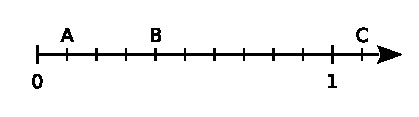
\includegraphics[width=7cm]{axe0AB1C} \end{center}
\end{exercice}


\begin{exercice}
Sur la demi-droite graduée ci-dessous, place les points $O(0)$, $A(1)$, $B(2)$, $C(0,5)$, $D(1,6)$, $E(0,1 + 0,05)$, $F(0,2)$, $G(1 + 0,05)$ et $H(1,45)$ :
\begin{center} 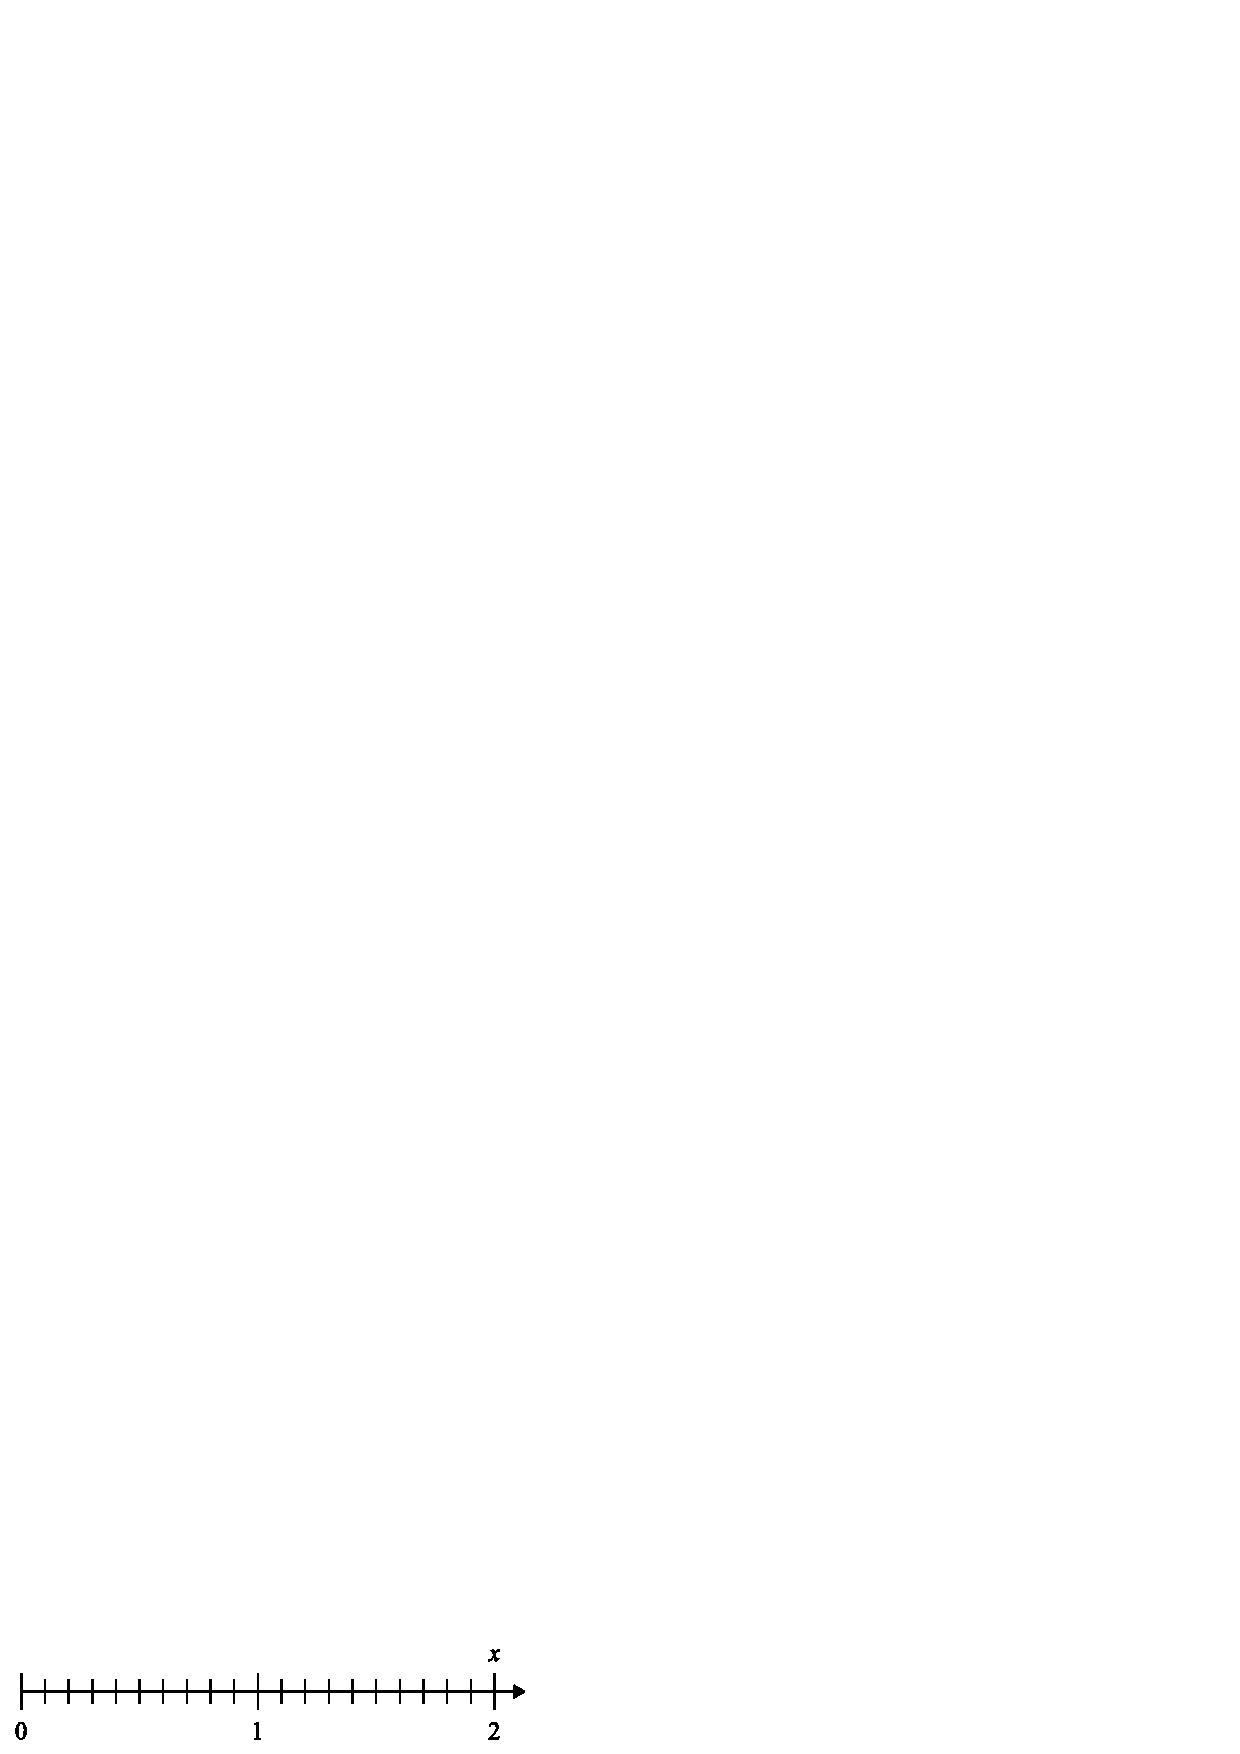
\includegraphics[width=7cm]{axe012x} \end{center}
\end{exercice}

%%%%%%%%%%%%%%%%%%%%%%%%%%%%%%%%%%%%%%%%%%%%%%%%%%%%%%%%%%%%%%%%%%%%%%%%%%%

\serie{Comparaison}

\begin{exercice}[Demi-droite graduée et comparaison]
\begin{enumerate}
 \item Reproduis la demi-droite graduée suivante et place les points $A(7,39)$ ; $B(7,46)$ et $C(7,425)$ :
\begin{center} 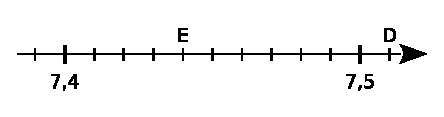
\includegraphics[width=6.6cm]{axe74E-75D} \end{center}
 \item Range dans l'ordre décroissant les abscisses de tous les points qui sont nommés.
 \end{enumerate}
\end{exercice}



%%%%%%%%%%%%%
\newpage    %
%%%%%%%%%%%%%



\begin{exercice}[Rangement]
Range les nombres suivants dans l'ordre croissant :

5 ; 4,99 ; 4,9 ; 4,88 ; 5,000 1 ; 4,909 ; 4,879 :

\dotfill

\dotfill
\end{exercice}


\begin{exercice}[Rangement $(bis)$]
Range les nombres suivants dans l'ordre décroissant :

120 ; 119,999 ; 120,000 1 ; 120,101 ; 119,9 ; 119 ; 119,990 9 ; 120,100 1 ; 102,01 ; 120,1 :

\dotfill

\dotfill
\end{exercice}

%%%%%%%%%%%%%%%%%%%%%%%%%%%%%%%%%%%%%%%%%%%%%%%%%%%%%%%%%%%%%%%%%%%%%%%%%%%

\serie{Arrondir}

\begin{exercice}[Arrondir à l'unité]
Arrondis à l'unité les nombres suivants :
\begin{enumerate}
 \item 46,8 \dotfill ; 
 
 \item 109,75 \dotfill ; 
 
 \item 1,3 \dotfill ; 
 
 \item 0,09 \dotfill ; 
 
 \item 234,08 \dotfill ; 
 
 \item 4\,087,63 \dotfill. 
 
 \end{enumerate}
\end{exercice}


\begin{exercice}[Arrondir à la dizaine]
Arrondis à la dizaine les nombres suivants :
\begin{enumerate}
 \item 234,2 \dotfill ; 
 
 \item 3,14 \dotfill ; 
 
 \item 17,62 \dotfill ; 
 
 \item 889,3 \dotfill ; 
 
 \item 6\,289,3 \dotfill ; 
 
 \item 23,005 \dotfill. 
 
 \end{enumerate}
\end{exercice}


\begin{exercice}[Arrondir au dixième]
Arrondis au dixième les nombres suivants :
\begin{enumerate}
 \item 8,372 \dotfill ; 
 
 \item 50,64 \dotfill ; 
 
 \item 30,18 \dotfill ; 
 
 \item 43,725 \dotfill ; 
 
 \item 0,02 \dotfill ; 
 
 \item 78,66 \dotfill. 
 
 \end{enumerate}
\end{exercice}


%%%%%%%%%%%%%%%%%%%%%%%%%%%%%%%%%%%%%%%%%%%%%%%%%%%%%%%%%%%%%%%%%%%%%%%%%%%



%%%%%%%%%%%%%
\vspace{6em}%
%%%%%%%%%%%%%


\serie{Encadrer}


\begin{exercice}[Encadrer à la dizaine]
235,5 ; 45 ; 1270 ; 574,23 ; 10\,095.
\end{exercice}


\begin{exercice}[Encadrer au dixième]
76,123 ; 461,99 ; 1\,254,01 ; 3,93 ; 9,99.
\end{exercice}



\begin{exercice}
Dans chaque cas, propose, si cela est possible, un nombre entier que l'on peut intercaler entre les deux nombres donnés. 
Y a‑t‑il plusieurs solutions ? Si oui, cite‑les :
\begin{enumerate}
 \item $5 < …… < 6$ ;
 \item $6,4 < …… < 6,8$ ;
 \item $3,8 < …… < 5,3$ ;
 \item $6,5 < …… < 7,21$.
 \end{enumerate}
\end{exercice}


\begin{exercice}
Dans chaque cas, donne trois exemples différents de nombres décimaux que l'on peut intercaler entre les deux nombres donnés :
\begin{enumerate}
 \item $6 < …… < 7$ ;
 \item $4,5 < …… < 4,9$ ;
 \item $3,45 < …… < 3,48$ ;
 \item $6,8 < …… < 6,9$ ;
 \item $15,13 < …… < 15,14$ ;
 \item $3,238 < …… < 3,24$.
 \end{enumerate}
\end{exercice}


\begin{exercice}[Chiffres masqués]
Certains chiffres sont masqués par \#. Lorsque cela est possible, complète les pointillés avec $<$,$>$ ou $=$ :
\begin{enumerate} 
 \item $6,51 …… 6,7\#$ ;
 \item $5,42 …… 5,0\#$ ;
 \item $\#,23 …… 4,16$ ;
 \item $6,04 …… 6,1\#$ ;
 \item $3,\#35 …… 3,01$ ;
 \item $43,\#96 …… 43,0\#$.
 \end{enumerate}
\end{exercice}


\begin{exercice}[Nombres à trouver]
Dans chaque cas, complète les pointillés par un nombre décimal :
\begin{enumerate} 
 \item $24,5 < ...... < 24,6$ ;  
 
 \item $12,99 < ...... < 13$ ; 
 
 \item $32,53 < ...... < 32,54$ ; 
 
 \item $58 < ...... < 58,01$ ; 
 
 \item $5,879 < ...... < ...... < ...... < 5,88$. 

 \end{enumerate}
\end{exercice}

%%%%%%%%%%%%%%%%%%%%%%%%%%%%%%%%%%%%%%%%%%%%%%%%%%%%%%%%%%%%%%%%%%%%%%%%%%%



%%%%%%%%%%%%%
\newpage    %
%%%%%%%%%%%%%



\serie{Techniques opératoires}


\begin{exercice}
Calcule mentalement les additions :
\begin{enumerate} 
 \item $4,6 + 5,2$ \dotfill ; 
 
 \item $6,2 + 3,4$ \dotfill ; 
 
 \item $4,5 + 6,1$ \dotfill ; 
 
 \item $8,3 + 9,6$ \dotfill ; 
 
 \item $8 + 1,5$ \dotfill ; 
 
 \item $8,6 + 8,9$ \dotfill ; 
 
 \item $3,9 + 5,4$ \dotfill ; 
 
 \item $6,5 + 8,7$ \dotfill ; 
 
 \item $6,8 + 9,4$ \dotfill ; 
 
 \item \hspace{0.1em} $12,9 + 15,8$ \dotfill. 

 \end{enumerate}
\end{exercice}


\begin{exercice}
Calcule mentalement les soustractions :
\begin{enumerate} 
 \item $6,5 - 4,3$ \dotfill ; 
 
 \item $7,6 - 0,4$ \dotfill ; 
 
 \item $4,9 - 4,3$ \dotfill ; 
 
 \item $5,7 - 0,4$ \dotfill ; 
 
 \item $4,7 - 4,3$ \dotfill ; 
 
 \item $6,2 - 4,6$ \dotfill ; 
 
 \item $9 - 8,7$ \dotfill ; 
 
 \item $3,1 - 1,8$ \dotfill ; 
 
 \item $7,8 - 6,9$ \dotfill ; 
 
 \item \hspace{0.2em}$17,4 - 8,7$ \dotfill. 
 
 \end{enumerate}  
\end{exercice}


\begin{exercice}
Calcule les sommes en effectuant des regroupements astucieux :
\begin{enumerate} 
 \item $6,5 + 12,6 + 1,5$ ;
 \item $36,99 + 45,74 + 2,01 + 13,26$ ;
 \item $9,25 + 8,7 + 5,3 + 16,75$ ;
 \item $34,645 + 34,75 + 2,25 + 4,355$ ;
 \item $7,42 + 4,2 + 7,8 + 25,58$ ;
 \item $3,01 + 2,9 + 6,1 + 7,99 + 2,001$.
 \end{enumerate}
\end{exercice}


\begin{exercice}
Pose et effectue :
\begin{enumerate} 
 \item $853,26 + 4 038,3$ ;
 \item $52 + 8,63 + 142,8$ ;
 \item $49,3 + 7,432 + 12,7$ ;
 \item $948,25 - 73,2$ ;
 \item $9,8 - 0,073$ ;
 \item $83 - 43,51$.
 \end{enumerate} 
 \end{exercice}


\begin{exercice}
Calcule mentalement :
\begin{enumerate} 
 \item $4,357 \cdot 100$ \dotfill ; 
 
 \item $89,7 \cdot 1\,000$ \dotfill ; 
 
 \item $0,043 \cdot 10$ \dotfill ; 
 
 \item $0,28 \cdot 1\,000$ \dotfill ; 
 
 \item $39 \cdot 100$ \dotfill ; 
 
 \item $0,48 \cdot 10$ \dotfill ; 
 	
 \item $354 \cdot 10$ \dotfill ; 
 	
 \item $0,03 \cdot 10\,000$ \dotfill ; 
 
 \end{enumerate}
\end{exercice}


\begin{exercice}
Calcule mentalement :
\begin{enumerate} 
 \item $4\,338 : 10$ \dotfill ; 
 
 \item $1\,297 : 1\,000$ \dotfill ; 
 	
 \item $12,3 : 10$ \dotfill ; 
 
 \item $0,87 : 100$ \dotfill ; 
 	
 \item $3,8 : 1\,000$ \dotfill ; 
 
 \item $0,04 : 100$ \dotfill ; 
 	
 \item $354 : 10$ \dotfill ; 
 
 \item $12,5 : 100$ \dotfill. 
 
 \end{enumerate}
\end{exercice}


\begin{exercice}
Calcule mentalement :
\begin{enumerate} 
 \item $435,7 \cdot 0,1$ \dotfill ; 
 
 \item $18,73 \cdot 0,01$ \dotfill ; 
 
 \item $439,345 \cdot 0,001$ \dotfill ; 
 
 \item $0,28 \cdot 0,1$ \dotfill ; 
 
 \item $39 \cdot 0,001$ \dotfill ; 
 
 \item $0,8 \cdot 0,01$ \dotfill ; 
 
 \item $354 \cdot 0,001$ \dotfill ; 
 
 \item $0,03 \cdot 0,001$ \dotfill. 
 
 \end{enumerate}
\end{exercice}

\begin{exercice}
Calcule mentalement :
\begin{enumerate} 
 \item $48 \div 0,1$ \dotfill ; 
 
 \item $12,97 \div 0,01$ \dotfill ; 

 \item $12,3 \div 0,001$ \dotfill ; 
 
 \item $0,45 \div 0,1$ \dotfill ; 
 	
 \item $5,61 \div 0,0001$ \dotfill ; 
 	
 \item $0,056 \div 0,1$ \dotfill ; 
 
 \item $354 \div 0,001$ \dotfill ; 
 
 \item $0,5 \div 0,001$ \dotfill. 

 \end{enumerate}
\end{exercice}


\begin{exercice}
Complète par 10 ; 100 ; 1\,000 ; 10\,000 \ldots :
\begin{enumerate} 
 \item $8,79 \cdot \dotfill = 87,9$ ; 
 
 \item $4,35 \cdot \dotfill = 43\,500$ ; 
 
 \item $0,837 \cdot \dotfill = 8,37$ ; 
 
 \item $0,367 \cdot \dotfill = 3,67$ ; 
 
 \item $0,028 \cdot \dotfill = 0,28$ ; 
 
 \item $0,17 \div \dotfill = 0,017$ ; 
 
 \item $23 \div \dotfill = 0,23$ ; 
 
 \item $480 \div \dotfill = 4,8$ ; 
 
 \item $900 \div \dotfill = 0,09$ ; 
 
 \item \hspace{0.25em}$18\,000 \div \dotfill = 18$. 
 
 \end{enumerate}
\end{exercice}


\begin{exercice}
Complète par le signe opératoire qui convient :
\begin{colenumerate}{2}
 \item $0,8 \ldots 100 = 80$ ;
 \item $0,38 \ldots 10 = 0,038$ ;
 \item $47 \ldots 100 = 0,47$ ;
 \item $380 \ldots 10 = 38$ ;
 \item $5 \ldots 0,1 = 0,5$ ;
 \item $60\,000 \ldots 10 = 6\,000$ ;
 \item $4\,100 \ldots 100 = 4\,000$ ;
 \item $5\,600 \ldots 100 = 56$ ;
 \item $8 \ldots 0,01 = 0,08$ ;
 \item \hspace{0.25em}$100 \ldots 1,2 = 120$.
 \end{colenumerate} 
\end{exercice}


\begin{exercice}
Calcule mentalement en détaillant ta démarche :
\begin{enumerate} 
 \item $0,1 \cdot 14 \cdot 1\,000$ \dotfill ; 
 
 \item $2,18 \cdot 0,001 \cdot 100$ \dotfill ; 

 \item $1,8 \cdot 0,01 \cdot 10$ \dotfill ; 

 \item $4 •\cdot 0,01 \cdot 100$ \dotfill. 

 \end{enumerate} 
\end{exercice}


\begin{exercice}
Sachant que $48 \cdot 152 = 7\,296$, détermine les résultats des calculs :
\begin{enumerate} 
 \item $48 \cdot 1,52$ \dotfill ; 
 
 \item $4,8 \cdot 15,2$ \dotfill ; 
 
 \item $0,48 \cdot 0,152$ \dotfill ; 
 
 \item $0,048 \cdot 1\,520$ \dotfill. 

 \end{enumerate} 
\end{exercice}


\begin{exercice}
Calcule en regroupant astucieusement :
\begin{enumerate} 
 \item $0,8 \cdot 2 \cdot 0,6 \cdot 50$ \dotfill ; 
 
 \item $0,25 \cdot 12,38 \cdot 4$ \dotfill ; 
 
 \item $8 \cdot 49 \cdot 1,25$ \dotfill ; 
 
 \item $2,5 \cdot 12,9 \cdot 0,04$ \dotfill ; 
 
 \item $0,15 \cdot 70 \cdot 0,02$ \dotfill ; 
 
 \item $75 \cdot 0,06 \cdot 0,4$ \dotfill. 
 
 \end{enumerate} 
\end{exercice}


\begin{exercice}
Place correctement la virgule dans le résultat de la multiplication (en ajoutant éventuellement un ou des zéros) :
\begin{enumerate} 
 \item $12,8 \cdot  5,3 = \textcolor{PartieGeometrie}{6\,784}$ ;
 \item $28,7 \cdot 1,04 = \textcolor{PartieGeometrie}{29\,848}$ ;
 \item $0,15 \cdot 6,3 = \textcolor{PartieGeometrie}{945}$ ;
 \item $0,008 \cdot 543,9 = \textcolor{PartieGeometrie}{43\,512}$ ;
 \item $0,235 \cdot 0,132 = \textcolor{PartieGeometrie}{3\,102}$.
 \end{enumerate}
\end{exercice}


\begin{exercice}
Place la virgule dans le nombre écrit en \textcolor{BleuOuv}{bleu} pour que l'égalité soit vraie :
\begin{enumerate} 
 \item $3,42 \cdot \textcolor{BleuOuv}{271} = 9,268\,2$ ;
 \item $\textcolor{BleuOuv}{432} \cdot 0,614 = 26,524\,8$ ;
 \item $0,48 \cdot \textcolor{BleuOuv}{62} = 29,76$ ;
 \item $2,6 \cdot \textcolor{BleuOuv}{485} = 126,1$ ;
 \item $\textcolor{BleuOuv}{45} \cdot 29,232 = 131,544$.
 \end{enumerate}
\end{exercice}

\begin{exercice}
Pose et effectue les produits :
\begin{enumerate} 
 \item $2,08 \cdot 4,23$ \dotfill ; 
 
 \item $4,38 \cdot 5,7$ \dotfill ; 
 
 \item $6,93 \cdot 15,8$ \dotfill ; 
 
 \item $8,35 \cdot 0,18 $\dotfill.  
 \end{enumerate}
\end{exercice}


\begin{exercice} 
Calcule mentalement :
\begin{colenumerate}{2}
 \item $ 8,6 \div 2$ ;
 \item $ 24,8 \div 4$ ;
 \item $ 8,8 \div 8$ ;
 \item $ 7,7 \div 11$ ;
 \item $ 15,6 \div 3$ ;
 \item $ 63,6 \div 6$.
 \end{colenumerate}
\end{exercice}


\begin{exercice} 
Pose et effectue les divisions suivantes pour en trouver le quotient décimal exact :
\begin{enumerate} 
 \item $ 12,6 \div 6$ \dotfill ; 
 
 \item $ 28,48 \div 4$ \dotfill ; 

 \item $ 169,2 \div 3$ \dotfill ; 

 \item $ 0,162 \div 9$ \dotfill ; 

 \item $ 67,5 \div 4$ \dotfill ; 

 \item $ 9,765 \div 15$ \dotfill. 
 \end{enumerate}
\end{exercice}

\begin{exercice}[Valeurs approchées]
\vspace{-1em}
\begin{enumerate} 
 \item Pose et effectue les divisions suivantes jusqu'au millième :
 \begin{itemize}
  \item $12 \div 7$ \dotfill ; 
  
  \item $148,9 \div 12$ \dotfill ; 
  
  \item $13,53 \div 3$ \dotfill. 
  \end{itemize}
 \item Pose et effectue les divisions suivantes jusqu'au centième :
  \begin{itemize}
  \item $123,8 \div 7$ \dotfill ; 
  
  \item $235,19 \div 11$ \dotfill ; 
  
  \item $0,14 \div 3$ \dotfill. 
  \end{itemize}
 \end{enumerate}
\end{exercice}


\begin{exercice} 
Calcule la valeur exacte ou une valeur arrondie au centième des divisions suivantes :
\begin{enumerate} 
 \item $1 \div 2,74$ \dotfill ; 

 \item $5,87 \div 2,3$ \dotfill ; 

 \item $3,24 \div 1,7$ \dotfill ; 

 \item $45,6 \div 0,24$ \dotfill ; 

 \item $20,35 \div 8,5$ \dotfill ; 

 \item $0,53 \div 0,17$ \dotfill. 
 \end{enumerate}
\end{exercice}


\begin{exercice} 
Calcule la valeur exacte ou une valeur arrondie au centième des divisions suivantes :
\begin{enumerate} 
 \item $3,35 \div 0,42$ \dotfill ; 

 \item $41,5 \div 3,14$ \dotfill ; 

 \item $ 0,03 \div 2,1$ \dotfill ; 

 \item $0,35 \div 0,25$ \dotfill ; 

 \item $0,53 \div 0,8$ \dotfill ; 

 \item $21,7 \div 0,14$ \dotfill. 
 \end{enumerate}
\end{exercice}

%%%%%%%%%%%%%%%%%%%%%%%%%%%%%%%%%%%%%%%%%%%%%%%%%%%%%%%%%%%%%%%%%%%%%%%%%%%

\serie{Heures, minutes, secondes}



\begin{exercice}
Convertis en heures et minutes :\\
78 min ; 134 min ; 375 min ; 35 min ; 3\,840 s.
\end{exercice}


\begin{exercice}
Effectue les calculs :
\begin{enumerate} 
 \item 3 h 25 min $+$ 5 h 33 min ;
 \item 12 h 28 min $-$ 9 h 17 min ;
 \item 6 h 38 min $+$ 19 h 53 min ;
 \item 21 h 15 min $-$ 9 h 29 min ;
 \item 5 h 13 min 33 s $+$ 9 h 45 min 47 s ;
 \item 9 h 6 min 15 s $-$ 8 h 39 min 36 s.
 \end{enumerate}
\end{exercice}


\begin{exercice}
Pose et effectue les opérations suivantes :
\begin{enumerate} 
 \item 18 h 15 min 22 s $+$ 9 h 37 min 43 s ;
 \item 12 h 26 min 52 s $-$ 7 h 39 min 57 s ;
 \item 9 h 38 min 22 s $+$ 4 h 59 min 34 s ;
 \item 12 h 40 min 21 s $-$ 6 h 35 s.
 \end{enumerate}
\end{exercice}


\begin{exercice}
Pose et effectue les opérations suivantes :
\begin{enumerate} 
 \item 13 h 25 min 42 s $+$ 12 h 35 min 52 s ;
 \item 15 h 43 min 08 s $-$ 6 h 51 min 34 s ;
 \item 10 h 41 s $+$ 9 h 57 min 49 s ;
 \item 21 h $-$ 17 h 31 min 32 s.
 \end{enumerate}
\end{exercice}


\begin{exercice}
Un randonneur part en promenade à 9 h 30. Il rentre à 12 h 05, ne s'étant arrêté pour se reposer que lors de trois pauses de 5 min chacune. Pendant combien de temps ce randonneur a‑t‑il marché ?
\end{exercice}


\begin{exercice}
Pierre part de chez lui à 9 h 55 pour aller faire des courses. Il met 12 min pour se rendre au supermarché et il y reste pendant 1 h 35 min.
\begin{enumerate} 
 \item À quelle heure repart‑il du supermarché ?
 \item Il rentre ensuite chez lui et y arrive à 12 h 01. Combien de temps son trajet de retour a‑t‑il duré ?
 \end{enumerate}
\end{exercice}


\begin{exercice}
Sarah a noté les heures de lever et de coucher du Soleil en septembre 2008. Le $1^{er}$ septembre, le Soleil s'est levé à 7 h 09 et il s'est couché à 20 h 31. Le 30 septembre, le Soleil s'est levé à 7 h 50 et il s'est couché à 19 h 30. De quelle durée les jours ont‑ils diminué au mois de septembre 2008 ?
\end{exercice}
 

\end{colonne*exercice}


\exercicesappr
\begin{colonne*exercice}
\begin{exercice}
Antoine possédait 832,25 CHF sur son livret d'épargne. Pour son anniversaire, ses parents y ont déposé 75 CHF. Combien a-t-il maintenant sur son livret ?
\end{exercice}


\begin{exercice}
Un panier plein de fruits pèse 1,836 kg. Vide, il pesait 0,425 kg. Quelle est la masse des fruits contenus dans ce panier ?
\end{exercice}


\begin{exercice}
Pierre a relevé le compteur de sa voiture au départ et au retour de vacances. Au départ, le compteur indiquait 58\,257,6 km. Au retour, il indiquait 59\,329,1 km. Quelle distance a‑t‑il parcourue pendant ses vacances ?
\end{exercice}


\begin{exercice}
Simon veut acheter un livre. Il a 25,35 CHF dans son porte‑monnaie et il lui manque 5,25 CHF pour acheter ce livre. Quel est le prix du livre ?
\end{exercice}


\begin{exercice}
Une voiture consomme 8,5 l d'essence pour faire 100 km. Combien d'essence consomme‑t‑elle pour faire 500 km ?
\end{exercice}
  
  
\begin{exercice}
Un employé gagne 17,25 CHF de l'heure. Il travaille 35 heures par semaine. Combien gagne‑t‑il chaque semaine ?
\end{exercice}


\begin{exercice}
Au marché, Anne a déposé dans son panier 1,2 kg de carottes, 600 g de raisin et 1,3 kg de pommes. Combien pèse le contenu de son panier ?
\end{exercice}


\begin{exercice}
Pour aller au collège, Caroline fait 1,4 km avec son vélo qu'elle laisse chez sa grand‑mère. Puis elle parcourt 150 m à pied jusqu'au collège. Quelle distance totale parcourt‑elle pour se rendre au collège ?
\end{exercice}


\begin{exercice}
Djamel a acheté 1,6 kg de poires à 2,30 CHF le kg. Combien a‑t‑il payé ?
\end{exercice}


\begin{exercice}
Gérard a payé 41,40 CHF pour 12 pieds de tomate. Quel est le prix d'un pied de tomate ?
\end{exercice}



\begin{exercice}
Un lot de six stylos identiques coûte 8,10 CHF. Quel est le prix d'un stylo ?
\end{exercice}


\begin{exercice}
Mercredi après‑midi, Anh Hao a fait cinq tours d'un circuit de VTT. Il a parcouru en tout 23,5 km. Quelle est la longueur de ce circuit ?
\end{exercice}


\begin{exercice}
Mme Betty possède 6,6 litres de jus de pomme. Combien de bouteilles de 0,7 litres pourra-t-elle remplir ?
\end{exercice}

\begin{exercice}
Agan possède 37,40 CHF en pièces de 20 centimes. Combien de pièces de 20 centimes possède t'il ?
\end{exercice}


\begin{exercice}[Énigme]
Trouve le nombre décimal à six chiffres tel que :
\begin{itemize}
 \item son chiffre des unités est 2 ;
 \item l'un de ses chiffres est 6 et sa valeur dans l'écriture décimale est cent fois plus petite que celle du chiffre 2 ;
 \item son chiffre des dizaines est le double de celui des unités et son chiffre des dixièmes est le quart de celui des dizaines ;
 \item ce nombre est compris entre 8\,975,06 et 9\,824,95 ;
 \item la somme de tous ses chiffres est égale à 27.
 \end{itemize}
\end{exercice}



\begin{exercice}[Nombres croisés]
Recopie et complète la grille à l'aide des nombres que tu trouveras grâce aux définitions :

\begin{center}
\begin{tabularx}{.5\linewidth}{r|c|c|c|c|c|}
\multicolumn{1}{c}{}& \multicolumn{1}{c}{\textbf{A}} & \multicolumn{1}{c}{\textbf{B}} & \multicolumn{1}{c}{\textbf{C}} & \multicolumn{1}{c}{\textbf{D}} & \multicolumn{1}{c}{\textbf{E}} \\ \cline{2-6}
\textbf{I} & & & & \cellcolor{black} & \\ \cline{2-6} 
\textbf{II} & & & & & \\ \cline{2-6} 
\textbf{III} & & \cellcolor{black} & & & \\ \cline{2-6} 
\textbf{IV} & & & & & \cellcolor{black} \\ \cline{2-6} 
\textbf{V} & \cellcolor{black} & & & & \\ \cline{2-6} 
\end{tabularx}
\end{center}

\vspace{0.75em}

\textbf{Horizontalement}

\textbf{I} : La partie entière de 328,54. Le chiffre des centièmes de 634,152.

\textbf{II} : Son chiffre des dizaines est le triple de celui des unités.

\textbf{III} : Le chiffre des dixièmes de 34. Arrondi à l'unité de 178,356.

\textbf{IV} : Entier compris entre 8\,000 et 9\,000.

\textbf{V} : Quarante-deux centaines.

\vspace{0.75em}

\textbf{Verticalement}

\textbf{A} : $(3 \cdot 1 000) + (5 \cdot 100) + (8 \cdot 1)$.

\textbf{B} : Le nombre de dixièmes dans 2,6. La partie entière de 2\,498 centièmes.

\textbf{C} : Quatre-vingt-six milliers et cent deux unités.

\textbf{D} : En additionnant tous les chiffres de ce nombre, on trouve 20.

\textbf{E} : Arrondi à l'unité près de 536,57. Entier qui précède 1.

\end{exercice}


\begin{exercice}
Voici les résultats (en secondes), pour les hommes, du 100 m aux JO de Pékin en 2008 : \vspace{0.75em}

Martina : 9,93 ; Frater : 9,97 ; Burns : 10,01 ; Patton : 10,03 ; Bolt : 9,69 ; Powell : 9,95 ; Thompson : 9,89 ; Dix : 9,91.\vspace{0.75em}

Classe les coureurs dans l'ordre décroissant de leur résultat.
\end{exercice}


\begin{exercice}[À ordonner]
Range les nombres suivants dans l'ordre croissant : \vspace{0.75em}

25 unités et deux dixièmes ; 2\,504 centièmes; $25 + 2$ centièmes ; deux mille cinquante‑deux centièmes ; 20,54 ; 254 dixièmes.
\end{exercice}


\begin{exercice}[À placer]
En choisissant judicieusement la longueur d'une graduation, place précisément sur une demi‑droite graduée les points $A$, $B$, $C$, $D$ et $E$ d'abscisses respectives : \\[0.75em]
12,02 ; mille deux cent treize centièmes ; $12 + 7$ centièmes ; 1\,198 centièmes ; cent vingt-et-un dixièmes.
\end{exercice}


\begin{exercice}[Comparaison]
\begin{enumerate}
 \item Quel est le plus grand nombre décimal ayant un chiffre après la virgule et inférieur à 83 ?
 \item Quel est le plus petit nombre décimal avec trois chiffres après la virgule et supérieur à 214,3 ?
 \item Quel est le plus grand nombre décimal avec deux chiffres après la virgule, ayant tous ses chiffres différents et qui est inférieur à 97,8 ?
 \item Quel est le plus petit nombre décimal avec trois chiffres après la virgule, ayant tous ses chiffres différents et qui est supérieur à 2\,341 ?
 \end{enumerate}
\end{exercice}


\begin{exercice} 
Voici les masses de lipides et glucides (en g) contenues dans 50 g de différents biscuits :

\begin{center}
\begin{tabularx}{\linewidth}{|c|*{6}{>{\centering \arraybackslash}X|}}
\hline \rowcolor{U1} Biscuit & A & B & C & D & E \\
\hline \cellcolor{U1} Lipides & 9,527 & 9,514 & 9,53 & 9,521 & 9,6 \\
\hline \cellcolor{U1} Glucides & 32,43 & 33 & 33,6 & 33,15 & 33,50 \\
\hline
\end{tabularx} \\
\end{center}

\begin{enumerate}
 \item Classe ces biscuits selon l'ordre croissant de leur quantité de lipides ;
 \item Classe ces biscuits selon l'ordre décroissant de leur quantité de glucides.
 \end{enumerate}
\end{exercice}


\begin{exercice}[Calculer sans poser]
\begin{enumerate}
 \item Calcule mentalement les produits suivants sachant que $6,5 \cdot 3,7 = 24,05$ :
 \begin{colitemize}{3}
  \item $6,5 \cdot 37$ ;
  \item $65 \cdot 37$ ;
  \item $6,5 \cdot 0,37$ ;
  \item $0,65 \cdot 3,7$ ;
  \item $6\,500 \cdot 0,003\,7$ ;
  \item $65 \cdot 0,37$.
  \end{colitemize}
  
 \item Sachant que $935 : 17 = 55$, que dire des quotients suivants ? Justifie.   
 \begin{colitemize}{2}
  \item $9 350 : 170$ ;
  \item $93,5 : 1,7$ ;
  \item $93\,500 : 1\,700$ ;
  \item $9,35 : 0,17$.
  \end{colitemize}
 \end{enumerate}
\end{exercice}


\begin{exercice}[Calculer sans poser (bis)]
\begin{enumerate}
 \item Calcule $96,5 + 83,7$ et $96,5 - 83,7$ ;
 \item Déduis‑en les sommes et les différences suivantes sans poser les opérations :
 \begin{colitemize}{2}
  \item $965 + 837$ ;
  \item $0,965 + 0,837$ ;
  \item $9,65 - 8,37$ ;
  \item $96\,500 - 83\,700$.
  \end{colitemize}
 \item Peut‑on trouver par ce moyen les résultats des opérations $96\,500 + 8\,370$ et $9\,650 - 837$ ? Pourquoi ?
 \end{enumerate}
\end{exercice}


\begin{exercice}[Que de restes !]
\begin{enumerate}
 \item Dans une planche de 478,8 cm de long, on veut découper des étagères de 9 cm de long :
 
Combien d'étagères peut‑on découper ? 

Quelle est la longueur du morceau restant ? 

\begin{center} 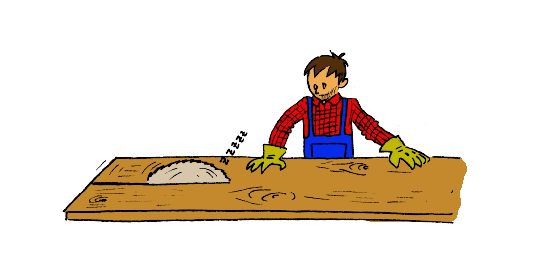
\includegraphics[width=5cm]{menuisier} \end{center}

Complète alors l'égalité $478,8 = 9 \cdot \ldots + \ldots$ . \label{NbEntDec_Approf81Qa}

 \item En utilisant la division écrite au \ref{NbEntDec_Approf81Qa}, recopie et complète les égalités suivantes :
 \begin{itemize}  
  \item $47,88 = 9 \cdot 5,3 + \ldots$ ;
  \item $4 788 = 9 \cdot 532 + \ldots$ ;
  \item $4 788 = 90 \cdot 53 + \ldots$ ;
  \item $4,788 = 9 \cdot \ldots + 0,018$.
  \end{itemize}
 \end{enumerate}
\end{exercice}


\begin{exercice}[Paquets empilés]
On a reçu au collège 7 rames de 500 feuilles pour la photocopieuse et 3 paquets de 24 pièces de « carton plume » :
\begin{enumerate}
 \item L'épaisseur d'une feuille de papier pour photocopieuse est de 0,11 mm et celle d'une pièce de « carton plume » est de 5 mm. Calcule un ordre de grandeur de la hauteur totale de tous ces paquets empilés ;
 \item Écris la hauteur totale des paquets en une seule expression puis calcule‑la.
 \end{enumerate}
\end{exercice}


\begin{exercice}[Densité de population]
On considère le tableau suivant :

\begin{center}
\begin{tabularx}{\linewidth}{|c|*{6}{>{\centering \arraybackslash}X|}}
\hline \rowcolor{U1} Continent & Nombre d'habitants & Superficie en km\up{2} \\
\hline \rowcolor{A3} Afrique & 965 millions & 30\,206\,704 \\
\hline \rowcolor{A3} Amérique & 911 millions & 42\,189\,120 \\
\hline \rowcolor{A3} Asie & 4,03 milliards & 43\,810\,582 \\
\hline \rowcolor{A3} Europe & 731 millions & 10\,180\,000 \\
\hline \rowcolor{A3} Océanie & 34 millions & 9\,008\,458 \\
\hline
\end{tabularx} \\
\end{center}

\begin{enumerate}
 \item Quel est le continent qui a le plus grand nombre d'habitants ? Et le plus petit nombre ?
 \item Quel est le continent qui a la plus grande superficie ? Et la plus petite ?
 \item Pour chaque continent, calcule la densité de population exprimée en habitants par km\up{2}. Tu donneras une valeur approchée à l'unité. 
 \item Ces résultats sont‑ils surprenants ? Explique.
 \item Calcule le nombre moyen d'habitants au km\up{2} dans le monde. Indique les continents qui sont en dessous de cette moyenne et ceux qui sont au dessus. 
 \end{enumerate}
\end{exercice}


\begin{exercice}[Football]
Le match de football entre le FC Barcelone et le Milan AC a eu lieu mardi soir 1\up{er} novembre à Barcelone. 
\begin{enumerate}
 \item Sachant qu’un match de football se joue en 2 mi-temps de 45 minutes séparées par une pause de 15 minutes, qu’il y a eu en tout 4 minutes d’arrêt de jeu en première mi-temps et 3 minutes en seconde mi-temps et que la rencontre a débuté à 20h45, trouver l’heure à laquelle le match s’est terminé. 
 \item Yvan, joueur de FC Barcelone est sorti du terrain au bout de 22 minutes de jeu en deuxième mi-temps, calculer l’heure à laquelle ce changement a eu lieu.
 \item Les supporters du Milan AC, qui avaient effectué le déplacement en autocar ont quitté le stade à 23h15 min. Sachant que leur voyage de retour a duré 16h40, calculer l’heure exacte et la date précise à laquelle ils sont arrivés à Milan. 
 \end{enumerate}
\end{exercice}
\end{colonne*exercice}

\connaissances
\begin{acquis}
\begin{itemize}
\item BlaBla1
\item BlaBla2
\item BlaBla3
\item BlaBla4
\item BlaBla5
\item BlaBla6
\end{itemize}
\end{acquis}

%%%%%%%%%%%%%%%%%%%%%%%%%%%%%%%%%%%%%%%%%%%%%%%%%%%%%%%%%%%%%%%%%%%%%%%%%%%

\QCMautoevaluation{Pour chaque question, plusieurs réponses sont % enlever l'adresse internet.
  proposées.  Déterminer celles qui sont correctes.} 

\begin{QCM}
  \begin{GroupeQCM} 
    \begin{exercice}
      Dix-huit millions huit cents s'écrit :
      \begin{ChoixQCM}{4}
      \item 18\,800\,000
      \item 18\,000\,800
      \item 18\,800
      \item 18\,008\,100
      \end{ChoixQCM}
\begin{corrige}
     \reponseQCM{a} % J'ai mis "a" partout
   \end{corrige}
    \end{exercice}

    \begin{exercice}
      45 centaines est égal à :
      \begin{ChoixQCM}{4}
      \item 5 unités
      \item 450 dizaines
      \item 4 dizaines
      \item 45\,100
      \end{ChoixQCM}
      \begin{corrige}
     \reponseQCM{a}
   \end{corrige}
    \end{exercice}

    
    \begin{exercice}
      Un centième est :
      \begin{ChoixQCM}{4}
      \item plus grand qu'un dixième
      \item égal à dix millièmes
      \item plus petit qu'un millième
      \item égal à dix  dixièmes
      \end{ChoixQCM}
      \begin{corrige}
     \reponseQCM{a}
   \end{corrige}
    \end{exercice}


    \begin{exercice}
      Une écriture décimale de 456 centièmes est :
      \begin{ChoixQCM}{4}
      \item 456,100
      \item 456\,100
      \item 4,56
      \item 4\,560 millièmes
      \end{ChoixQCM}
      \begin{corrige}
     \reponseQCM{a}
   \end{corrige}
    \end{exercice}


    \begin{exercice}
      Le nombre $5 + 0,4 + 0,007$ peut aussi s'écrire :
      \begin{ChoixQCM}{4}
      \item 547 millièmes
      \item 5,47
      \item 5,407
      \item 5\,047 millièmes
      \end{ChoixQCM}
      \begin{corrige}
     \reponseQCM{a}
   \end{corrige}
    \end{exercice}
    
     \begin{exercice}
      7 unités, 8 centièmes et 5 millièmes s'écrit :
      \begin{ChoixQCM}{4}
      \item 7,85
      \item 7,085
      \item 7,800\,500\,0
      \item 7,085\,0
      \end{ChoixQCM}
      \begin{corrige}
     \reponseQCM{a}
   \end{corrige}
    \end{exercice}

     \begin{exercice}
      Dans l'écriture décimale du nombre 45,631...
      \begin{ChoixQCM}{4}
      \item la valeur du chiffre 3 est dix fois moins grande que celle du chiffre 6
      \item 6 est le chiffre des centaines
      \item la valeur du chiffre 4 est deux fois plus grande que celle du chiffre 6
      \item 0,631 est la partie décimale
      \end{ChoixQCM}
      \begin{corrige}
     \reponseQCM{a}
   \end{corrige}
    \end{exercice}

     \begin{exercice}
      Un nombre compris entre 24,56 et 24,57 est par exemple...
      \begin{ChoixQCM}{4}
      \item 24\,568 millièmes
      \item 24,560\,7
      \item impossible, il n'y a pas de nombre compris entre 24,56 et 24,57
      \item $42 + 0,562$
      \end{ChoixQCM}
      \begin{corrige}
     \reponseQCM{a}
   \end{corrige}
    \end{exercice}
    
     \begin{exercice}
      L'arrondi de 123,254 au dixième est...
      \begin{ChoixQCM}{4}
      \item 120
      \item 123,2
      \item 123,26
      \item 123,3
      \end{ChoixQCM}
      \begin{corrige}
     \reponseQCM{a}
   \end{corrige}
    \end{exercice}

     \begin{exercice}
      873,023 est ...
      \begin{ChoixQCM}{4}
      \item 1\,000 fois plus grand que 873\,230
      \item 100 fois plus petit que 87\,302,3
      \item 10\,000 fois plus grand que 0,087\,302\,3
      \item 10 fois plus petit que 87,302\,3
      \end{ChoixQCM}
      \begin{corrige}
     \reponseQCM{a}
   \end{corrige}
    \end{exercice}
    
     \begin{exercice}
      $57,41 - 27,83 =$ ...
      \begin{ChoixQCM}{4}
      \item 30.42
      \item 30.58
      \item 29.58
      \item 19.58
      \end{ChoixQCM}
      \begin{corrige}
     \reponseQCM{a}
   \end{corrige}
    \end{exercice}
 \end{GroupeQCM}  
 \end{QCM}  
    
    
    
    
    
 \begin{QCM}
\begin{GroupeQCM}
     \begin{exercice}
      $872,967 =$ ...
      \begin{ChoixQCM}{4}
      \item $87\,296,7 \div 100$
      \item $862,967 \cdot10$
      \item $87,296\,7 \cdot 10$
      \item $8,729\,67 \cdot 100$
      \end{ChoixQCM}
      \begin{corrige}
     \reponseQCM{a}
   \end{corrige}
    \end{exercice}
    
     \begin{exercice}
      $78,23 \cdot 21,796 =$ ...
      \begin{ChoixQCM}{4}
      \item 170\,510,108
      \item 3\,705,101\,08
      \item 1\,705,101\,08
      \item 1\,800
      \end{ChoixQCM}
      \begin{corrige}
     \reponseQCM{a}
   \end{corrige}
    \end{exercice}
    
     \begin{exercice}
      $34,1 + 123,79$ se pose ...
      \begin{ChoixQCM}{4}
      \item 
      
      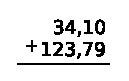
\includegraphics[width=1.5cm]{frac1}
      \item 
      
      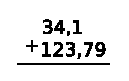
\includegraphics[width=1.5cm]{frac2}
      \item 
      
      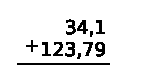
\includegraphics[width=1.7cm]{frac3}
      \item 
      
      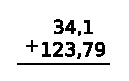
\includegraphics[width=1.5cm]{frac4}
      \end{ChoixQCM}
      \begin{corrige}
     \reponseQCM{a}
   \end{corrige}
    \end{exercice}

    
     \begin{exercice}
      Une ficelle mesure 7,2 m. On la partage en 16.
      \begin{ChoixQCM}{4}
      \item Chaque bout mesure 1,152 m
      \item C'est impossible, $16 > 7,2$
      \item Chaque bout mesure environ 2,2 m
      \item Chaque bout mesure 45 cm
      \end{ChoixQCM}
      \begin{corrige}
     \reponseQCM{a}
   \end{corrige}
    \end{exercice}
    
    \begin{exercice}
      0,75 peut être la réponse du (ou des) problème(s) suivant(s) :
      \begin{ChoixQCM}{4}
      \item Avec 126 litres d'eau, on a rempli 168 bouteilles. Quelle est la contenance d'une bouteille ?
      \item Une baignoire peut contenir 223,24 L. On la remplit avec  222,49 L d'eau. Combien d'eau peut‑on encore verser ?
      \item Ahmed achète un bonbon à 0,27 CHF et un chewing‑gum à 0,58 CHF. Combien paye‑t‑il ?
      \item 125 CD de 6 mm d'épaisseur sont empilés. Quelle est la hauteur en mètre de la pile ?
      \end{ChoixQCM}
      \begin{corrige}
     \reponseQCM{a}
   \end{corrige}
    \end{exercice}
    
    \begin{exercice}
      Henri court pendant 1 h 52 min. Il s'arrête à 10 h 07. Il est parti à...
      \begin{ChoixQCM}{4}
      \item 8 h 55
      \item 11 h 59
      \item 8 h 15
      \item 9 h 45
      \end{ChoixQCM}
      \begin{corrige}
     \reponseQCM{a}
   \end{corrige}
    \end{exercice}

\end{GroupeQCM}
\end{QCM}

  

\TravauxPratiques % pour nous "travailler en groupe"

\begin{TP}[]
Voici un extrait de « La Disme », écrit par Simon Stevin en 1585 : \\[0.3em]

« Les 27 \circled{0} 8 \circled{1} 4 \circled{2} 7 \circled{3} donnés, font ensemble 27 $\dfrac{8}{10}$, $\dfrac{4}{100}$, $\dfrac{7}{1\,000}$, ensemble 27 $\dfrac{847}{1\,000}$, et par même raison les 37 \circled{0} 6 \circled{1} 7 \circled{2} 5 \circled{3} valent 37 $\dfrac{675}{1\,000}$. Le nombre de multitude des signes, excepté \circled{0}, n'excède jamais le 9. Par exemple nous n'écrivons pas 7 \circled{1} 12 \circled{2}, mais en leur lieu 8 \circled{1} 2 \circled{2}. »

\partie{Simon Stevin}

Par groupe, en vous documentant, répondez aux questions suivantes.
\begin{enumerate}
 \item Où Simon Stevin a-t-il vécu ?
 \item Quels sont les domaines dans lesquels Simon Stevin a travaillé ? Faites la synthèse des réponses de chaque groupe.

\partie{La Disme} % Pourquoi cette ligne est si rentrée ?

\item Cherchez comment on écrit de nos jours le nombre 38 \circled{0} 6 \circled{1} 5 \circled{2} 7 \circled{3}­.

Comparez avec les réponses des autres groupes.

\item Écrivez, à la manière décrite par Simon Stevin, les nombres $124 + \dfrac{7}{10} + \dfrac{5}{100}$ et 34,802.

Comparez avec les réponses des autres groupes.

 \item Choisissez trois nombres décimaux différents et écrivez-les à la manière décrite par Simon Stevin.
 \item échangez ensuite avec un autre groupe ces nombres écrits à la manière de Simon Stevin. Cherchez alors comment on écrit de nos jours les nombres que vous avez reçus.
 \item Faites une recherche pour trouver les différentes notations utilisées depuis 1585 pour l'écriture des nombres décimaux.
 \end{enumerate}
\end{TP}

%%%%%%%%%%%%%%%%%%%%%%%%%%%%%%%%%%%%%%%%%%%%%%%%%%%%%%%%%%%%%%%%%%%%%%%%%%%

\begin{TP}[Compétitions dans la classe]
Préparatifs : fabriquez une étiquette de carton pour chaque élève de la classe, comportant son nom et son prénom. Mélangez ces étiquettes.

Voici un exemple de liste de calculs à effectuer :
\begin{enumerate}
 \item $853,12 + 19,7$ ;
 \item $538,21 - 42,16$ ;
 \item $65,24 \cdot 7,38$ ;
 \item $68,37 : 3$.
 \end{enumerate}

\partie{Entraînement en individuel (appelé 1 contre 10)}
Pour chaque manche, un élève $A$ est tiré au sort à l'aide des étiquettes et passe au tableau où un seul calcul écrit est à effectuer. \\[0.5em]
L'élève $A$ l'effectue en public pendant que tous les autres cherchent chacun sur une feuille. \\[0.5em]
Dès qu'un élève a trouvé la réponse et a écrit le calcul, il lève la main. Le professeur surveille le tableau et circule dans la classe pour vérifier le travail de chaque élève. \\[0.5em]
Il compte à haute voix de 1 à 10 en ajoutant 1 chaque fois qu'un travail est considéré comme correct. \\[0.5em]
Arrivé à 10, si l'élève $A$ n'a pas trouvé, la classe a gagné la manche. Par contre, si l'élève $A$ trouve avant la fin du décompte à 10, c'est lui qui a gagné.

\partie{Par équipes (appelé 2 contre 5)}
On constitue des binômes équilibrés d'élèves.\\[0.5em]
Lors du tirage au sort, l'élève $A$ désigné passe au tableau accompagné de son coéquipier mais seul l'élève $A$ peut écrire. \\[0.5em]
On démarre la compétition comme dans le « 1 contre 10 » mais le professeur ne compte que jusqu'à 5. 
\end{TP}

\pagebreak

\Recreation
\begin{enigme}[La constante de Champernowne]

Ce nombre, inventé par le mathématicien anglais David Gawen Champernowne en 1933, commence par

0,123456789101112131415 \ldots . \\[-1em]
\begin{enumerate}
 \item Quelle est la particularité de cette constante ? Donne les dix décimales suivantes.
 \item Quelle est l'arrondi, au cent-milliardième près, de cette constante ?
 \end{enumerate}
 \end{enigme}
        
\vspace*{2em}
        
\begin{enigme}[Défis]
Combien de fois faudrait-il utiliser le chiffre 1 si l'on voulait écrire tous les nombres entiers de 1 à 999 ? Et le chiffre 9 ?

Donne le nombre de mots utilisés pour écrire tous les entiers plus petits que 100.
 \end{enigme} 
 
 \vspace*{2em}

\begin{enigme}[Calculatrices infernales 1 (d'après Apmep)]
Sur la calculatrice d'Aïsha, la touche pour afficher la virgule ne fonctionne plus et la touche « $=$ » ne peut fonctionner qu'une seule fois par ligne de calcul.

Comment peut‑elle trouver le résultat de $(17,32 \cdot 45,3) + 15,437$ ?
 \end{enigme} 
 
 \vspace*{2em}

\begin{enigme}[Calculatrices infernales 2 (d'après Apmep)]
Bruce vient de faire tomber sa calculatrice. Elle ne comporte plus que les chiffres, la virgule et les quatre opérations, mais quand on appuie sur « $+$ » elle ajoute 1, quand on appuie sur « $-$ » elle retranche 1, quand on appuie sur la touche « $\times$ » elle multiplie par 10 et quand on appuie sur la touche « $\div$ » elle divise par 10. \\[-1em]
\begin{enumerate}
 \item Romain emprunte la calculatrice de Bruce. Il tape 27,2 puis appuie ensuite sur les touches « $\times$ », « $\times$ », « $+$ », « $+$ », « $-$ », « $\div$ », « $\div$ », « $\div$ », « $+$ », « $\times$ ». Quel résultat Romain trouve-t-il ?
 \item Comment peut‑il passer en sept opérations :    
 \begin{colitemize}{3}
  \item de 3,14 à 300 ?
  \item de 3,14 à 297 ?
  \item de 297 à 0,2 ?
  \end{colitemize}
 \item Tu viens de passer de 3,14 à 0,2 en quatorze opérations. Trouve un chemin qui permette de faire cela avec le minimum d'opérations. Compare avec tes camarades ; \\[0.5em]
Trouve un chemin qui permette de passer de 5 à 4,99 en un minimum d'opérations puis compare avec tes camarades.
 \end{enumerate}
\end{enigme} 





\themaG
\chapter{Points, segments, droites, cercles et angles}

\activites

\begin{activite}[Segments, droites et demi-droites]

 \begin{partie}[À la découverte d'un nouveau code]
  \begin{enumerate}
   \item Lire la consigne de la case \circled{1} et observer la figure correspondant à cette consigne.
Faire de même pour la case \circled{2}.

Quand le code est compris, tracer la figure de la case \circled{3} et écrire la consigne de la case \circled{4}.


  \vspace{1em}
  
  
  
  \begin{tabular}{|c|c|c|c|c|}
  \cline{1-2}\cline{4-5}
    \circled{1} 		& \circled{2} 		& 	& \circled{3} 		& \circled{4}	\\ 
     Tracer $(AB)$ 	&  Tracer $[AC)$ 	& 	& Tracer $(AB)$	& 	 		\\ 
     Tracer $[AC]$ 	& Tracer $[BC]$ 	& 	& Tracer$[BC]$		& 			\\
     				&				&	& Tracer$[AC)$		&			\\ \cline{1-2}\cline{4-5}
   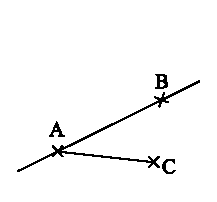
\includegraphics[width=.2\linewidth]{tracerAB-AC} & 
   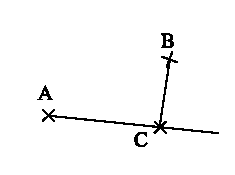
\includegraphics[width=.2\linewidth]{tracerAC-BC} & & 
   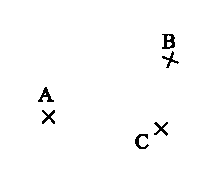
\includegraphics[width=.2\linewidth]{tracerAB-BC-AC}& 
   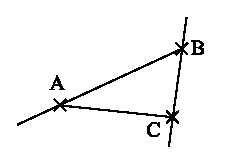
\includegraphics[width=.2\linewidth]{tracer} 					\\ \cline{1-2}\cline{4-5}
  \end{tabular}\\[1em]

  
   \item Lire la consigne de la case \circled{5} et observer la figure correspondant à cette consigne. Tracer ensuite la figure de la case \circled{6} et écrire la consigne de la case \circled{7}.
   
   \vspace{1em}
  
    \begin{tabular}{|l|l|l|}
   \hline
    \hfill \circled{5} \hfill			&	\hfill \circled{6} \hfill				&	\hfill \circled{7} \hfill 	\\
    - Tracer la droite passant par 	&	- Tracer le segment 				&					\\
    $E$ et $F$ ;					&	d'extrémités $R$ et $S$ ;			&					\\
    - Tracer le segment 			&	- Tracer la droite passant par 		&					\\
    d'extrémités $E$ et $G$ ;		&	$R$ et $T$ ;					&					\\
    - Tracer la demi-droite 			&	- Tracer la demi-droite 			&					\\
    d'origine $G$ et passant par $F$.	&	d'origine $S$ et passant par $T$.	&					\\ \hline
    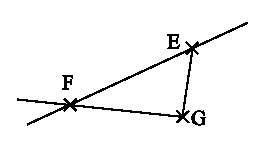
\includegraphics[width=.24\linewidth]{tracerEFG} 			&  
    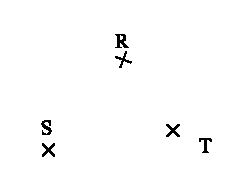
\includegraphics[width=.24\linewidth]{tracerRST}			&
    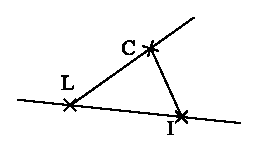
\includegraphics[width=.24\linewidth]{tracerLCI}			\\ \hline
    \end{tabular}\\[1em]

    
  \newpage
  
   \item Compléter le tableau suivant :
   
   \vspace{1em}
   
   \renewcommand*\tabularxcolumn[1]{>{\centering\arraybackslash}m{#1}}
   \begin{ttableau}{\linewidth}{3}
    \hline
    \multicolumn{1}{|c|}{\textbf{Phrase}}	&	\multicolumn{1}{c}{\textbf{Phrase codée}}	&	\multicolumn{1}{|c|}{\textbf{Dessin}}			 	\\  \hline
    								&	Tracer $[UV]$							&	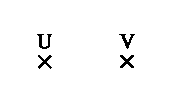
\includegraphics[width=2.6cm]{phraseUV}		\\  \hline
    								&										&	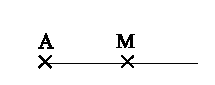
\includegraphics[width=3.2cm]{phraseAM}		\\  \hline
   Tracer la droite passant par $S$ et $T$	&										&	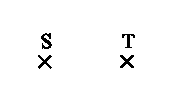
\includegraphics[width=2.6cm]{phraseST}		\\  \hline
   								&										&	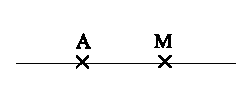
\includegraphics[width=4.0cm]{phraseAM_2}	\\  \hline
   Tracer le segment d'extrémités $M$ et $N$	&									&	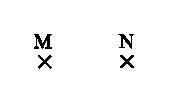
\includegraphics[width=2.6cm]{phraseMN} 	\\  \hline
   								&	Tracer $[KJ)$							&	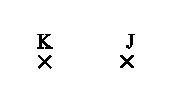
\includegraphics[width=2.6cm]{phraseKJ}		\\  \hline
								&										&	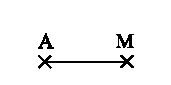
\includegraphics[width=2.6cm]{phraseAM_3}	\\  \hline
   Tracer la demi-droite d'origine $O$ et 	&										&	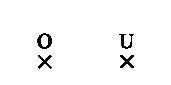
\includegraphics[width=2.6cm]{phraseOU}		\\
   passant par $U$					&										&										\\  \hline
   								&	Tracer $(BC)$							&	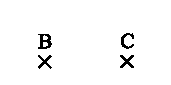
\includegraphics[width=2.6cm]{phraseBC}		\\  \hline
  \end{ttableau}
  
   \end{enumerate} 

  \end{partie}

\end{activite}

\newpage

%%%%%%%%%%%%%%%%%%%%%%%%%%%%%%%%%%%%%%%%%%%%%

\begin{activite}[Repérer des droites perpendiculaires]

 \begin{minipage}[c]{0.50\linewidth}
  \begin{partie}[Éric a oublié son équerre !]
 
  « Pas de souci, lui dit son professeur, prends une feuille blanche non quadrillée. Tu devrais pouvoir obtenir un angle droit en pliant deux fois cette feuille. »
  
  Réalise une telle équerre.
  
  Qu'obtiens‑tu si tu déplies ta feuille ? 
    \end{partie}
  
  \begin{partie}[Éric utilise sa nouvelle équerre \ldots]
  
  Éric doit replacer l'équerre dans la position qui a permis de construire les droites $d_4$ et $d_7$. \\[0.5em]
  Place l'équerre dans cette position. \\[0.5em]
  Trouve alors un autre couple de droites \textbf{perpendiculaires} sur cette figure en t'aidant de ton équerre.
    \end{partie} \end{minipage} \hfill %
   \begin{minipage}[c]{0.44\linewidth}
   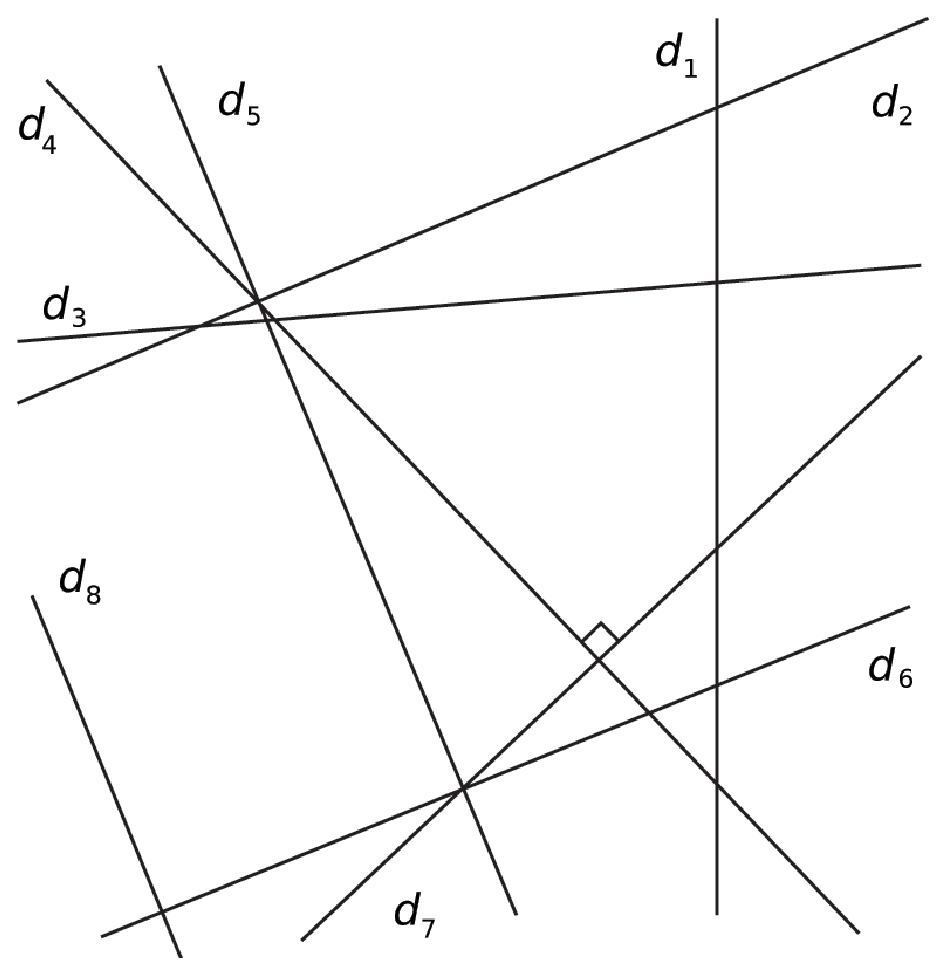
\includegraphics[width=6.1cm]{plusieurs_droites}
   \end{minipage} \\

 \begin{partie}[Utilisation de l'équerre d'Éric]
 
Trace deux droites sécantes $d$ et $d'$. À l'aide de l'équerre que tu as fabriquée, construis une droite perpendiculaire à $d$ et une autre perpendiculaire à $d'$. Tu n'oublieras pas d'ajouter les codages nécessaires.

  \end{partie} 
  
\end{activite}

%%%%%%%%%%%%%%%%%%%%%%%%%%%%%%%%%%%%%%%%%%%%%

\begin{activite}[Droites parallèles]

 \begin{partie}[Deux droites perpendiculaires]
 
  \begin{enumerate}
   \item Place deux points $A$ et $B$.
   \item Trace une droite $d$ ne passant ni par $A$, ni par $B$ et qui coupe $(AB)$.
   \item Trace $d_1$ la perpendiculaire à d passant par $A$, puis la droite $d_2$ perpendiculaire à $d_1$ passant par $B$. Que remarques‑tu ?
   \item Trace $d_3$ la perpendiculaire à $d$ passant par $B$ et $d_4$ la perpendiculaire à $d_3$ passant par $A$. Que peux‑tu dire de $d_2$ et $d_4$ ? Quelles autres remarques du même type peux‑tu faire ? 
   \end{enumerate}
   
  \end{partie} 

 \begin{partie}[Construction à la règle et à l'équerre]
 
 \begin{minipage}[c]{0.66\linewidth}
 La première vignette d'une bande dessinée est représentée ci‑contre. On y a placé une droite $d$ et un point $A$ n'appartenant pas à $d$.
 Complète cette bande dessinée pour expliquer comment, à l'aide de la règle et de l'équerre, tu traces la \textbf{parallèle} à $d$ passant par $A$.
  \end{minipage} \hfill %
 \begin{minipage}[c]{0.3\linewidth}
 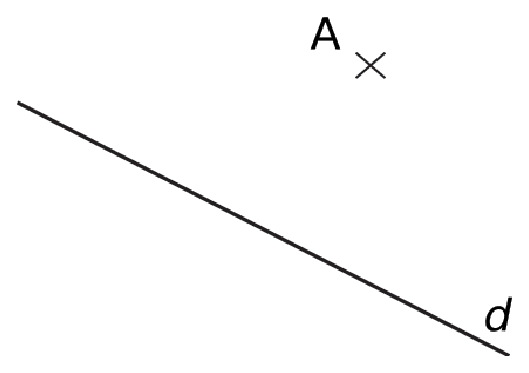
\includegraphics[width=4.2cm]{droiteAd}
  \end{minipage} \\
 
  \end{partie} 

\end{activite}

%%%%%%%%%%%%%%%%%%%%%%%%%%%%%%%%%%%%%%%%%%%%%

\begin{activite}[Tout savoir sur la médiatrice !]

 \begin{partie}[Axes de symétrie d'un segment]
 
 \begin{enumerate}
  \item Sur une feuille blanche, trace un segment $[AB]$.
  \item Plie cette feuille de manière à ce que le point $A$ touche le point $B$, cela fait apparaître un axe de symétrie de ce segment. Le symétrique de $A$ par rapport à cet axe est $B$. Comment s'appelle cet axe ? Repasse‑le en couleur.
  \item Quelles sont ses caractéristiques ?
  \end{enumerate}
  
  \end{partie}
  
 \begin{partie}[Propriété d'un point appartenant à la médiatrice d'un segment]
 
 \begin{enumerate}
  \item Place un point $M$ sur cette médiatrice. Que dire des longueurs $AM$ et $BM$ ?
  \item Que dire alors d'un point qui appartient à la médiatrice d'un segment ?
  \end{enumerate}
  
  \end{partie}
  
 \begin{partie}[Ensemble de points]
 
 \begin{minipage}[c]{0.76\linewidth}
 \begin {enumerate}
  \item Construis un segment $[CD]$ de longueur 5 cm. 
  \item Place $A$, \textbf{équidistant} de $C$ et de $D$. Place trois autres points équidistants de $C$ et de $D$. 
  \item Où semblent se trouver tous les points équidistants de $C$ et $D$ ?
  \item Que dire d'un point équidistant des extrémités d'un segment ?
  \item Déduis‑en une façon de construire la médiatrice d'un segment sans l'équerre. 
  \end{enumerate} 
  \end{minipage} \hfill %
 \begin{minipage}[c]{0.2\linewidth}
 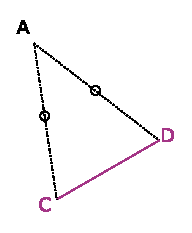
\includegraphics[width=2.8cm]{triangleACD}
  \end{minipage} \\
  
 \end{partie}

\end{activite}

%%%%%%%%%%%%%%%%%%%%%%%%%%%%%%%%%%%%%%%%%%%%%

\begin{activite}[Bissectrice, qui es-tu ?]

 \begin{partie}[Définition] \label{EntDroitSeg_DefBissectrice}

 \begin{minipage}[c]{0.68\linewidth}
 \begin {enumerate}
  \item Sur une feuille blanche, trace un angle $\widehat{ABC}$.
  \item Plie cette feuille de façon à faire apparaître l'axe de symétrie de l'angle. Repasse‑le en couleur. Place un point D sur cet axe (comme sur le croquis ci contre). \label{EntDroitSeg_plier}
  \item Cet axe fait apparaître deux nouveaux angles. Nomme‑les.
  \item Que peut‑on dire de la mesure de ces deux angles ? Justifie. Comment nomme‑t‑on cette droite ?
  \end{enumerate} 
  \end{minipage} \hfill %
 \begin{minipage}[c]{0.26\linewidth}
 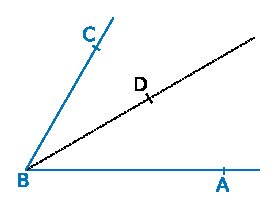
\includegraphics[width=3.8cm]{bissectrice}
  \end{minipage} \\
  
 \end{partie}
 
 \begin{partie}[Construction au compas]
 
 \begin{enumerate}
 \item Construis le point $A'$ symétrique du point $A$ par rapport à la bissectrice de l'angle $\widehat{ABC}$ Tu obtiens ce point en reportant le point A sur la droite $[BC)$ en pliant la feuille comme au point \ref{EntDroitSeg_plier} de la partie \ref{EntDroitSeg_DefBissectrice}. Que dire des longueurs $BA$ et $BA'$ ?
 \item Que représente la bissectrice de l'angle $\widehat{ABC}$ pour le segment $[AA']$ ?
 \item Déduis‑en une façon de construire la bissectrice d'un angle sans rapporteur.
  \end{enumerate}              
  \end{partie}
 
\end{activite}

%%%%%%%%%%%%%%%%%%%%%%%%%%%%%%%%%%%%%%%%%%%%%

\begin{activite}[De qui est-ce la trace ?]

 \begin{partie}
 Sur ton cahier, place un point $O$. Recherche tous les points situés à 3 cm du point $O$. 
  \end{partie}

 \begin{partie}
 \begin{minipage}[c]{0.78\linewidth}
 Un système d'arrosage automatique est formé d'un jet qui arrose dans toutes les directions jusqu'à 4 m.
  \begin {enumerate}
  \item Représente sur ton cahier la zone arrosée par le jet en appelant $J$ l'emplacement du jet. (1 cm représentera 1 m.)
  \item Comment peux‑tu définir les points de la zone arrosée ? 
  \end{enumerate} 
  \end{minipage} \hfill %
 \begin{minipage}[c]{0.16\linewidth}
 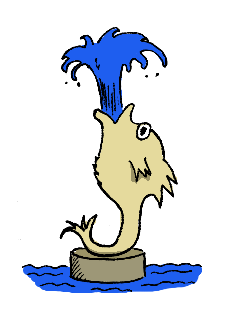
\includegraphics[width=2cm]{arrosage}
  \end{minipage} \\
    
  \end{partie}

\end{activite}

%%%%%%%%%%%%%%%%%%%%%%%%%%%%%%%%%%%%%%%%%%%%%

\begin{activite}[Des constructions]

 \begin{partie}[Du programme à la figure]
 Réalise la suite d'instructions suivantes :
 \begin{itemize}
  \item Trace un cercle $(\mathcal{C})$ de centre $O$ et de rayon 5 cm.
  \item Place, sur le cercle, deux points $A$ et $B$ \textbf{diamétralement opposés}.
  \item Construis le cercle $(\mathcal{C}_1)$ de diamètre $[OA]$ et le cercle $(\mathcal{C}_2)$ de diamètre $[OB]$.
  \item Trace le cercle $(\mathcal{C}_3)$ de centre $A$ passant par $O$.
  \item Nomme $E$ et $F$ les \textbf{points d'intersection} des cercles $(\mathcal{C})$ et $(\mathcal{C}_3)$.
  \item Trace le cercle $(\mathcal{C}_4)$ de centre $B$ et de rayon $OB$.
  \item Les cercles $(\mathcal{C})$ et $(\mathcal{C}_4)$ se coupent en $G$ et $H$.
  \end{itemize}
  
  \end{partie}
  
  \vspace{2em}
  
 \begin{partie}[De la figure au programme]
 \begin{minipage}[c]{0.48\linewidth} 
Construis la figure ci‑contre donnée 

par son croquis.

Écris le programme de construction.
 \end{minipage} \hfill %
 \begin{minipage}[c]{0.46\linewidth}
 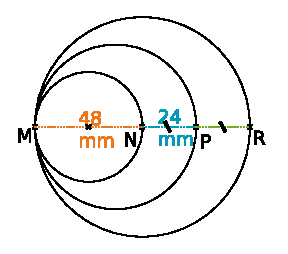
\includegraphics[width=4.2cm]{figure-programme}
  \end{minipage} \\
  
  \end{partie}

\end{activite}

%%%%%%%%%%%%%%%%%%%%%%%%%%%%%%%%%%%%%%%%%%%%%


\cours
\section{Les angles}

%%%%%%%%%%%%%%%%%%%%%%%%%%%%%

% remarque : pour qu'un mot se retrouve dans le lexique : \MotDefinition{asymptote horizontale}{} 

\begin{definition}
Un \MotDefinition{angle}{} est une portion de plan délimitée par deux demi-droites ayant la même origine.
 \end{definition}

\subsection{Reconnaître les différents types d'angles}

On classe les angles par catégories selon leur mesure.

 \renewcommand*\tabularxcolumn[1]{>{\centering\arraybackslash}m{#1}}
 \begin{ttableau}{\linewidth}{6}
\hline \textbf{Angle} 	&	Nul	&	Aigu		&	Droit		&	Obtus	&	Plat	\\ \hline
 \textbf{Figure} 	&	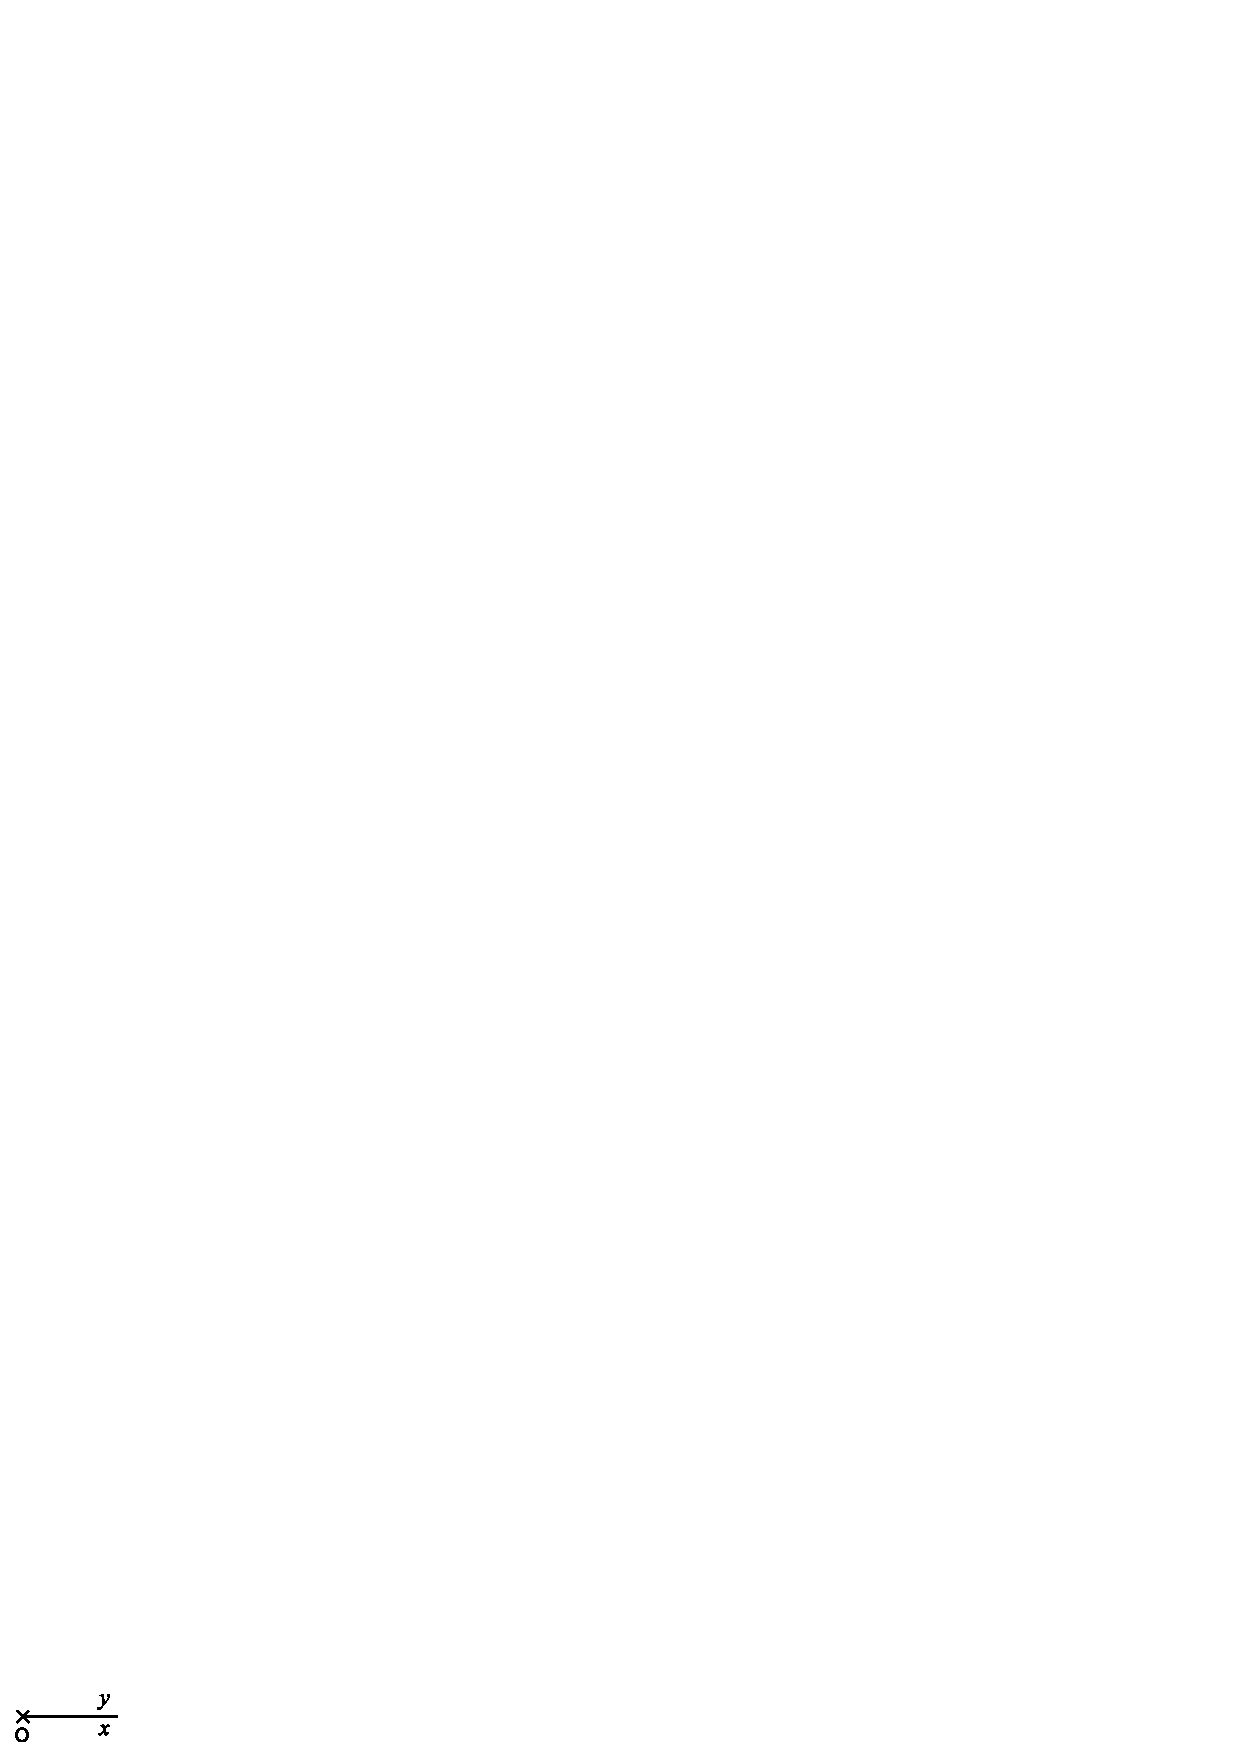
\includegraphics[width=1.7cm]{angle_nul}	&	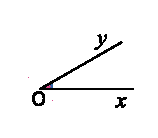
\includegraphics[width=1.7cm]{angle_aigu}	&	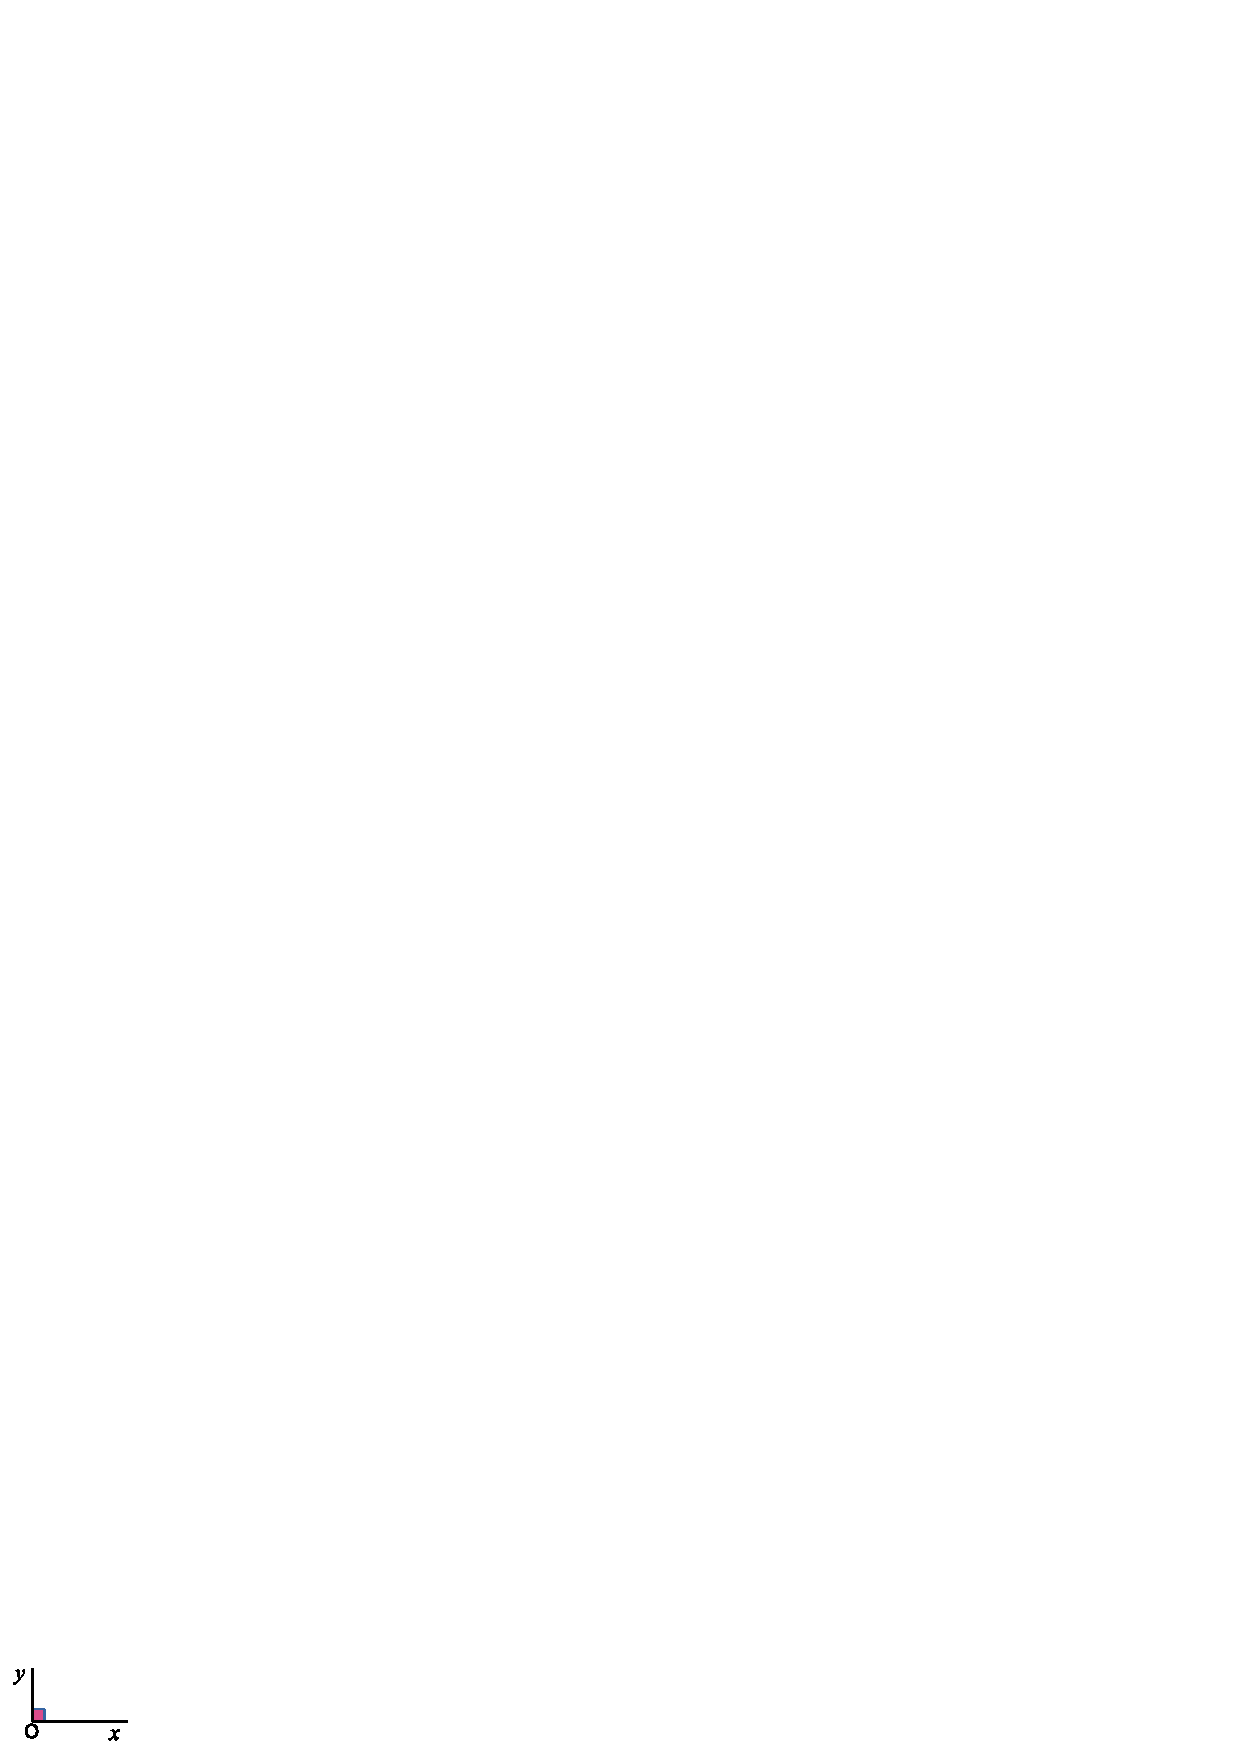
\includegraphics[width=1.7cm]{angle_droit}	&	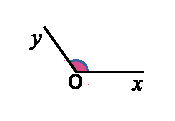
\includegraphics[width=1.7cm]{angle_obtus}	&	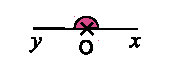
\includegraphics[width=1.7cm]{angle_plat}	\\ \hline
 \textbf{Mesure} 	&	$0^\circ$	&	entre $0^\circ$ et $90^\circ$	&	$90^\circ$		&	entre $90^\circ$ et $180^\circ$	&	 $180^\circ$	\\ \hline
 \multirow{3}{*}{\textbf{Position des côtés}} 	&		&	&	&	&	dans le 	\\ 
 	&	confondus		&	&	perpendiculaires	&	&	 prolongement	\\
	&	&	&	&	&	 l'un de l'autre	\\ \hline
 \end{ttableau}

%%%%%%%%%%%%%%%%%%%%%%%%%%%%%

\begin{methode*1}[Nommer un angle]

\begin{exemple*1}
Nomme l'angle marqué en violet sur la figure ci‑dessous.  \\[0.75em]

\begin{minipage}[c]{0.70\textwidth}
Le sommet de l'angle est le point $C$ : c'est la lettre centrale. \\[0.5em]
Les côtés de l'angle sont les demi‑droites $[CH)$ (ou $[Cx)$) et $[CS)$ (ou $[CA)$ (ou $[Cy)$). \\[0.5em]
Cet angle peut se nommer : $\widehat{{\textcolor{A1}{H}}C{\textcolor{C1}{S}}}$; $\widehat{{\textcolor{C1}{S}}C{\textcolor{A1}{H}}}$ ; $\widehat{{\textcolor{A1}{H}}C{\textcolor{C1}{A}}}$ ; $\widehat{{\textcolor{C1}{A}}C{\textcolor{A1}{H}}}$ ; $\widehat{{\textcolor{C1}{y}}C{\textcolor{A1}{x}}}$.
 \end{minipage} \hfill%
 \begin{minipage}[c]{0.26\textwidth}
 \includegraphics[width=3.8cm]{nommer_angle}
 \end{minipage} \\
 
\end{exemple*1}

\exercice 
Nomme les angles marqués sur la figure ci‑dessous. 
\begin{center} \includegraphics[width=4.5cm]{nommer_angles} \end{center}
%\correction
 
\end{methode*1}

%%%%%%%%%%%%%%%%%%%%%%%%%%%%%

\begin{methode*1}[Utiliser le rapporteur]

\begin{exemple*1}
Mesure l'angle $\widehat{CAB}$. \\[0.75em]

\begin{minipage}[c]{0.49\textwidth}
\centering
\includegraphics[width=4.8cm]{rapporteur1}
\end{minipage}\hfill%
 \begin{minipage}[c]{0.49\textwidth}%
 \centering
 \includegraphics[width=6.6cm]{rapporteur2}
  \end{minipage} \\
 \begin{minipage}[c]{0.43\textwidth}
On place le centre du rapporteur sur le sommet de l'angle.
\end{minipage} \hfill%
 \begin{minipage}[c]{0.53\textwidth}
 On place un zéro du rapporteur sur le côté $[AC)$. Si besoin, on prolonge la demi‑droite $[AC)$. La mesure de l'angle est donnée par l'autre côté de l'angle sur \underline{la même échelle} de graduation.
 \end{minipage} \\
  \end{exemple*1}
 
 \begin{exemple*1}
Construis un angle $\widehat{BUT}$ de $108^\circ$.  \\[0.75em]

\begin{minipage}[c]{0.49\textwidth}
\centering
\includegraphics[width=4.8cm]{rapporteur3}
\end{minipage}\hfill%
 \begin{minipage}[c]{0.49\textwidth}%
 \centering
 \includegraphics[width=6.6cm]{rapporteur4}
  \end{minipage} \\
 \begin{minipage}[c]{0.43\textwidth}
On trace $[UB)$, premier côté de l'angle. On place le centre du rapporteur sur le point $U$.
\end{minipage} \hfill%
 \begin{minipage}[c]{0.53\textwidth}
 On place un zéro du rapporteur sur le côté $[UB)$. On marque, d'un petit trait-repère, $108^\circ$ avec la bonne graduation.
On trace la demi‑droite d'origine $U$ passant par le repère. On place un point $T$ sur cette demi‑droite.
  \end{minipage} \\
  \end{exemple*1}
 
\exercice
 \begin{enumerate}
 \begin{minipage}[c]{0.36\textwidth}
  \item Mesure l'angle $\widehat{xOy}$ ci‑contre ;
  \item Construis un angle $\widehat{SAT}$ de $85^\circ$. 
  \end{minipage} \hfill%
 \begin{minipage}[c]{0.56\textwidth}
  \includegraphics[width=6cm]{angleyOx} 
  \end{minipage} \\
  \end{enumerate}
%\correction
 
\end{methode*1}

%%%%%%%%%%%%%%%%%%%%%%%%%%%%%

\section{Constructions graphiques : parallèles et perpendiculaires}

\begin{methode*1}[Construire la perpendiculaire à une droite passant par un point]

\begin{exemple*1}
Trace une droite $d$ et place un point $M$ n'appartenant pas à la droite $d$.

Trace la droite $d'$ perpendiculaire à la droite $d$ passant par le point $M$. \\[0.75em]

\begin{tabularx}{\textwidth}{X|X|X|X}
 \includegraphics[width=2.4cm]{droiteMxd} &  \includegraphics[width=2.4cm]{equerre} & \includegraphics[width=2.4cm]{regle} &  \includegraphics[width=2.4cm]{angledMd}\\ 
 On trace une droite $d$ et on place un point $M$. & On place l'un des côtés de l'angle droit de l'équerre sur la droite $d$ et l'autre côté sur $M$.
 & On prolonge la droite à la règle. & On nomme la droite $d'$ et on code l'angle droit par un carré.\\

\end{tabularx} \\
 
 \end{exemple*1}


\exercice

En utilisant cette méthode, tracer un rectangle ABCD de longueur 3 cm et de longueur 5 cm.

%\correction

 
\end{methode*1}

\newpage

%%%%%%%%%%%%%%%%%%%%%%%%%%%%%

\begin{methode*1}[Construire la parallèle à une droite passant par un point]

\begin{exemple*1}
Trace une droite $d$ et place un point $M$ n'appartenant pas à la droite $d$.

Trace la droite $d'$ parallèle à la droite $d$ passant par le point $M$. \\[0.75em]

\begin{tabularx}{\textwidth}{X|X|X|X}
 \includegraphics[width=2.4cm]{droiteMd} &  \includegraphics[width=2.4cm]{equerreMd} & \includegraphics[width=2.4cm]{equerre_regle} &  \includegraphics[width=2.4cm]{2droites}\\ 
On trace une droite $d$ et on place un point $M$. & On place l'un des côtés de l'angle droit de l'équerre sur la droite $d$. & On fait coulisser l'équerre le long de la règle, jusqu'au point $M$, sans bouger la règle. & On trace ainsi la droite $d'$.\\
\end{tabularx} \\
 
 \end{exemple*1}

\exercice 
Trace dans ton cahier un segment $[AB]$ d'une longueur de 5 cm et place un point $C$ au-dessus du segment $[AB]$ ($C$ n'est pas sur le segment). Construis, en rouge, la perpendiculaire à $[AB]$ passant par $C$. Construis, en vert, la parallèle à $[AB]$ passant par $C$.
%\correction

\end{methode*1}

%%%%%%%%%%%%%%%%%%%%%%%%%%%%%
\newpage

\section{La médiatrice}

\begin{definition}
La \textbf{\MotDefinition{médiatrice}{}} d'un segment est la droite qui coupe ce segment perpendiculairement en son milieu.
\end{definition}


\begin{methode*1}[Construire une médiatrice]

\begin{exemple*1}
Trace un segment $[OS]$ de longueur 5 cm puis sa médiatrice. \\[0.75em]

\begin{tabularx}{\textwidth}{X|X|X|X}
 \includegraphics[width=2.4cm]{segmentOS} &  \includegraphics[width=2.4cm]{milieu_segmentOS} & \includegraphics[width=2.4cm]{segmentOS_equerre} &  \includegraphics[width=2.4cm]{segmentOS_droit} \\ 
On trace un segment $[OS]$. & On trace le milieu du segment. & On trace la droite perpendiculaire au segment qui passe par ce milieu. & On code l'angle droit par un carré. \\
\end{tabularx} \\

 \end{exemple*1}
 
 \begin{exemple*1}
Trace un segment $[AB]$ de longueur 6 cm. Construis sa médiatrice au compas. \\[0.75em]

\begin{tabular}{l|l|l|l}
 \textcolor{H1}{\circled{1}} &  \textcolor{H1}{\circled{2}} &  \textcolor{H1}{\circled{3}} & \textcolor{H1}{\circled{1}} On trace le segment $[AB]$. \\ 
 \multirow{7}{*}{\includegraphics[width=2cm]{regleA}} &  \multirow{7}{*}{\includegraphics[width=1.5cm]{compasAB}} & \multirow{7}{*}{\includegraphics[width=1.5cm]{mediatriceAB}} &  \textcolor{H1}{\circled{2}} On trace deux arcs de cercle de \\ % exemple de fusion de cellules d'une même colonne
&&&  centres $A$ et $B$, de même rayon \\ 
&&& en choisissant un rayon \\
&&& suffisamment grand pour que ces \\
 &&& arcs se coupent en deux points. \\
&&& \textcolor{H1}{\circled{3}} La médiatrice de [AB] est la droite \\
&&&   qui passe par ces deux points.\\ 
\end{tabular} \\

 \end{exemple*1}

\exercice 
Trace un segment $[AB]$ de 7 cm. Trace la médiatrice du segment $[AB]$ par la méthode de ton choix.
%\correction

 
\end{methode*1}

%%%%%%%%%%%%%%%%%%%%%%%%%%%%%

\section{La bissectrice}

\begin{definition}
La \textbf{\MotDefinition{bissectrice}{}} d'un angle est l'axe de symétrie de cet angle.
\end{definition}


\begin{methode*1}[Construire une bissectrice]


\begin{exemple*1} \\[0.75em]
Trace un angle $\widehat{xOy}$. Construis sa bissectrice au compas. \\[0.5em]

\begin{tabularx}{\textwidth}{X|X|X}
 \includegraphics[width=2.4cm]{compasxOy} &  \includegraphics[width=2.4cm]{compas_arcsxOy} & \includegraphics[width=2.4cm]{bissectricexOy} \\ 
Au compas, on trace un arc de cercle de centre $O$ qui coupe chaque côté de l'angle en un point. & On trace deux arcs de cercle de même rayon ayant ces deux points pour centres. Ces arcs se coupent en un point. & La bissectrice de l'angle $\widehat{xOy}$ est la demi-droite d'origine $O$ passant par ce point. \\
\end{tabularx} \\

 \end{exemple*1}

\exercice 

Trace un triangle $ABC$ tel que $AB=4$\,cm ; $AC=7$\,cm ; $BC=5$\,cm ; puis trace les bissectrices des angles $\widehat{ABC}$ ; $\widehat{BAC}$ et $widehat{ACB}$. Que remarques-tu ?

%\correction

 
\end{methode*1}

%%%%%%%%%%%%%%%%%%%%%%%%%%%%%

\section{Le cercle}

\begin{definition}
Un \textbf{\MotDefinition{cercle}{}} de centre $O$ est l'ensemble des points situés à la même distance du point $O$. 
Cette distance est le \textbf{\MotDefinition{rayon}{}} du cercle.
\end{definition}

\begin{aconnaitre}
\begin{tabularx}{.95\linewidth}{|X|p{5cm}|p{3cm}|}
\hline
\multirow{5}{*}{\includegraphics[width=3.4cm]{cercleAFNME}}  & Le \textcolor{C2}{\textbf{centre}} d'un cercle est le point équidistant de tous les points qui constituent ce cercle. & Le point $O$ est le \textcolor{C2}{\textbf{centre}} du cercle $(\mathcal{C})$.\\ \cline{2-3}
 & Un \textcolor{J1}{\textbf{rayon}} d'un cercle est un segment ayant pour extrémités le centre et un point de ce cercle. & Le segment $[OA]$ est un  \textcolor{J1}{\textbf{rayon}} du cercle $(\mathcal{C})$.\\ \cline{2-3}
  & Un  \textcolor{H1}{\textbf{diamètre}} d'un cercle est un segment ayant pour extrémités deux points de ce cercle et contenant son centre. & Le segment $[EF]$ est un  \textcolor{H1}{\textbf{diamètre}} du cercle $(\mathcal{C})$.\\ \cline{2-3}
 & Une  \textcolor{PartieFonction}{\textbf{corde}} d'un cercle est un segment ayant pour extrémités deux points de ce cercle. & Le segment $[MN]$ est une  \textcolor{PartieFonction}{\textbf{corde}} du cercle $(\mathcal{C})$.\\ \cline{2-3}
 & Un  \textcolor{B2}{\textbf{arc de cercle}} est une portion de cercle comprise entre deux points de ce cercle. & La portion de cercle $\overset{\huge{\frown}}{MN}$ comprise entre $M$ et $N$ est un  \textcolor{B2}{\textbf{arc du cercle}} $(\mathcal{C})$.\\ \hline
  \end{tabularx}
 \end{aconnaitre}
  
  
 \begin{remarque}
 Par commodité de langage, on appelle « rayon » la longueur du rayon d'un cercle, et  on appelle « diamètre » la longueur de son diamètre.
  \end{remarque}
  
 \begin{remarque}
 Le diamètre d'un cercle est égal au double de son rayon.
  \end{remarque}

\newpage

\begin{methode*1}[Vocabulaire du cercle]

 \begin{exemple*1} \\[0.75em]
Trace le cercle de centre $T$ passant par le point $U$. \\[0.5em]

\begin{tabularx}{\linewidth}{X|X|X}
 \includegraphics[width=1.8cm]{pointsUT} &  \includegraphics[width=3.2cm]{compasUT} & \includegraphics[width=3.2cm]{cercleUT} \\ 
  & \multicolumn{1}{|p{3cm}|}{On pointe le compas sur le point $T$ et on écarte le compas jusqu'à ce que la mine soit sur le point $U$.} & On trace le cercle. \\
\end{tabularx} 

 \end{exemple*1}

\exercice 

Trace un rectangle $ABCD$ tel que $AB=6$\,cm et $BC=3$\,cm. Trace les segments $[AC]$ et $[BD]$. On appelle $O$ leur point d'intersection. Trace le cercle de centre $O$ passant par $A$. Que remarques-tu ?

%\correction

 
\end{methode*1}

%%%%%%%%%%%%%%%%%%%%%%%%%%%%%





\exercicesbase
\begin{colonne*exercice}

\serie{Points, segments et droites}

\begin{exercice}[Avec un quadrillage]
 \begin{center} \includegraphics[width=7.2cm]{quadrillage} \end{center}
 \begin{enumerate}
  \item En utilisant le quadrillage de ton cahier, place les points $A$, $B$, $C$ et $D$ comme sur la figure ci-dessus :
  \item Trace en bleu le segment $[AB]$ ;
  \item Trace en vert le segment d'extrémités $D$ et $C$ ;
  \item Trace en rouge la droite passant par $A$ et $C$ ;
  \item Trace en noir la demi-droite d'origine $D$ passant par $B$.
  \end{enumerate}
 \end{exercice}


\begin{exercice}[Appartient ou pas ?]
 \begin{center} \includegraphics[width=4.8cm]{droiteABECD} \end{center}
 Après avoir observé la figure, recopie et complète les pointillés avec $\in$ ou $\notin$ :
    \begin{colenumerate}{3}
     \item $B$ \ldots $[AC]$
     \item $D$ \ldots $[AB]$
     \item $E$ \ldots $[AD]$
     \item $B$ \ldots $[CA)$
     \item $D$ \ldots $[CA)$
     \item $E$ \ldots $[CE]$
     \end{colenumerate}
\end{exercice}


\begin{exercice}[À trouver]
 \begin{center} \includegraphics[width=6.5cm]{droiteFGHIJK}  \end{center}
 Parmi les points nommés sur la figure, indique ceux qui appartiennent à :
    \begin{colenumerate}{2}
     \item $[FK]$ ;
     \item $[IG)$ ;
     \item $[FJ]$ et à $[GK]$ ;
     \item $[GJ)$ mais pas à $[HJ]$ ;
     \item $[FG]$ ou à $[IJ)$ ;
     \item $[FH]$ et à $[JK]$.
     \end{colenumerate}
\end{exercice}


\begin{exercice}[Vrai ou faux ?]
 \begin{center} \includegraphics[width=4.6cm]{segmentsAB-CD}  \end{center}
 Observe cette figure composée de deux segments $[AB]$ et $[CD]$ sécants et indique pour chaque affirmation si elle est vraie ou fausse :
 \begin{enumerate}
  \item Les points $C$, $D$ et $M$ sont alignés ;
  \item $M$ est le point d'intersection des segments $[AB]$ et $[CD]$ ;
  \item $M$ est le milieu du segment $[AC]$ ;
  \item $M$ est un point du segment $[CD]$ ;
  \item $A$ appartient au segment $[MB]$ ;
  \item $M$ est le milieu du segment $[CD]$.
 \end{enumerate}
\end{exercice}


\begin{exercice}[Milieux]
\begin{enumerate} 
 \item Trace un segment $[RS]$ de longueur 4,8 cm et place son milieu $T$ ;
 \item Place un point $U$ qui ne soit pas aligné avec $R$ et $S$ ;
 \item Place le point $V$ tel que $T$ soit le milieu du segment $[UV]$.
 \end{enumerate}
\end{exercice}


\begin{exercice}[À construire]
\begin{enumerate} 
 \item Place trois points $A$, $B$ et $C$ non alignés ;
 \item Trace les segments $[BC]$ et $[AC]$ ;
 \item Marque le milieu $I$ du segment $[BC]$ et le milieu $J$ du segment $[AC]$ ;
 \item Trace le segment d'extrémités $B$ et $J$ ;
 \item Note $K$ le point d'intersection des segments $[AI]$ et $[BJ]$ ;
 \item Trace le segment $[AB]$ et place son milieu $L$. Trace enfin le segment $[CL]$. Que remarques‑tu ?
 \end{enumerate}
\end{exercice}


\begin{exercice}[À construire (bis)]
\begin{enumerate} 
 \item Place trois points $L$, $M$ et $N$ non alignés ;
 \item Place un point $A$ appartenant au segment $[LN]$ ;
 \item Place un point $B$ appartenant à la demi‑droite $[MN)$ mais n'appartenant pas au segment $[MN]$ ;
 \item Place le point $C$ aligné d'une part avec $A$ et $B$, et d'autre part avec $L$ et $M$.
 \end{enumerate}
\end{exercice}


\begin{exercice}[Bande dessinée]
 \begin{center} \includegraphics[width=4.3cm]{bande-dessinee}  \end{center}
Pour chaque étape de la bande dessinée, écris la consigne qui a été donnée, sans tenir compte des mesures.
\end{exercice}

%%%%%%%%%%%%%%%%%%%%%%%%%%%%%%%%%%%%%%%%%%%%%%%%%%%%%%%%%

\serie{Droites parallèles et perpendiculaires}

\begin{exercice}[Position de droites]
 \begin{center} \includegraphics[width=5.8cm]{mikado}  \end{center}
Observe la figure ci‑dessus et note sur ton cahier :
\begin{itemize}
 \item Le nom des droites qui \textbf{te semblent} perpendiculaires ;
 \item Le nom des droites qui sont sécantes mais non perpendiculaires ;
 \item Le nom des droites qui \textbf{te semblent} parallèles.
 \end{itemize}
\end{exercice}


\begin{exercice}[Position de droites $(bis)$]
 \begin{center} \includegraphics[width=7.3cm]{mikado2}  \end{center}
\begin{enumerate}
 \item Quelles sont les droites qui sont à coup sûr perpendiculaires ?
 \item Quelle semble être la position relative des droites $(BA)$ et $(GR)$ ?
 \end{enumerate}
\end{exercice}


\begin{exercice}[Quadrillage]
Reproduis une figure similaire à celle ci‑dessous. Trace, à la règle, la droite $d_1$ perpendiculaire à la droite $d$ passant par le point $M$ et la droite $d_2$ parallèle à la droite $d'$ passant par $M$.
\begin{center} \includegraphics[width=5.2cm]{quadrillage2}  \end{center}
\end{exercice}


\begin{exercice}[Constructions]
\begin{enumerate}
 \item Reproduis sur une feuille blanche les deux figures ci‑dessous :
 \begin{center} \includegraphics[width=6.1cm]{constructions}  \end{center}
 \item Pour chacune des figures, trace :
  \begin{itemize}
   \item La droite $d'$ perpendiculaire à $d$ et passant par $B$ ;
   \item La droite $d''$ perpendiculaire à $d$ et passant par $A$.
   \end{itemize}
 \item Que peux‑tu dire des droites $d'$ et $d''$ ?
 \end{enumerate}
\end{exercice}


\begin{exercice}[Constructions $(bis)$]
 \begin{center} \includegraphics[width=5.7cm]{constructions2}  \end{center}
\begin{enumerate}
 \item Reproduis la figure ci‑dessus ;
 \item Trace $d'$, la parallèle à $d$ passant par $A$ ;
 \item Trace $d''$, la parallèle à $d$ passant par $B$ ;
 \item Que peux‑tu dire des droites $d'$ et $d''$ ?
 \end{enumerate}
\end{exercice}


\begin{exercice}[Programme de construction]
\begin{enumerate}
 \item Place deux points $A$ et $B$ tels que $AB = 8$ cm ;
 \item Place un point $L$ sur $[AB]$ tel que $AL = 3$ cm ;
 \item Trace la droite $d$ telle que $L \in d$ et $(AB) \perp d$ ;
 \item Place un point $C$ tel que $C \in d$ et $LC = 2$ cm ;
 \item Trace la droite $d'$ telle que $d' \parallel (AB)$ et $C \in d'$ ;
 \item Sur la demi‑droite $[BC)$, place le point $I$ tel que $BI = 7$ cm ;
 \item Trace la droite $d''$ telle que $I \in d''$ et $d'' \parallel (AC)$.
 \end{enumerate}
\end{exercice}


\begin{exercice}
Construis la figure suivante : \\[0.75em]
\begin{minipage}[c]{0.2\textwidth}
\includegraphics[width=3.8cm]{constructions3}
 \end{minipage} \hfill%
 \begin{minipage}[c]{0.2\textwidth}
 $(BM) \parallel (AN)$
  \end{minipage} \\
\end{exercice}


\begin{exercice}
Reproduis la figure ci‑dessous en vraie grandeur : \\[0.75em]
\begin{minipage}[c]{0.2\textwidth}
\includegraphics[width=4.5cm]{double-triangle}
 \end{minipage} \hfill%
 \begin{minipage}[c]{0.2\textwidth}
$AB = 5,3$ cm ;
$BC = 3$ cm ;
$AC = 7,7$ cm.
 \end{minipage} \\
\end{exercice}

%%%%%%%%%%%%%%%%%%%%%%%%%%%%%%%%%%%%%%%%%%%%%%%%%%%%%%%%%

\serie{Médiatrice d’un segment}

\begin{exercice}[Médiatrices]
Dans chaque cas, trace le segment de longueur donnée puis sa médiatrice :
 \begin{colenumerate}{3}
  \item $AB = 2$ cm 
  \item $DE = 7,8$ cm
  \item $FG = 76$ mm
  \end{colenumerate}
\end{exercice}


\begin{exercice}[Points alignés]
 \begin{enumerate}
  \item Trace un segment $[AB]$ de longueur 7 cm ;
  \item Place le point $C$ de la demi‑droite $[BA)$ tel que $BC = 12$ cm ;
  \item Construis la médiatrice $m_1$ du segment $[AC]$ ;
  \item Construis la médiatrice $m_2$ du segment $[AB]$ ;
  \item Que remarques‑tu ?
  \end{enumerate}
\end{exercice}


\begin{exercice}[Reconnaître]
Sur chacune des figures ci‑dessous, indique si $P$ est sur la médiatrice de $[AB]$ : \\[0.5em]
 \begin{colenumerate}{2}
  \item 
  
  \includegraphics[width=2.2cm]{mediatriceAB1}
  \item 
  
  \includegraphics[width=2.2cm]{mediatriceAB2}
  \item 
  
  \includegraphics[width=2.2cm]{mediatriceAB3}
  \item 
  
  \includegraphics[width=2.2cm]{mediatriceAB4}
  \end{colenumerate}
\end{exercice}
 
 
\begin{exercice}[Construction]
 \begin{enumerate}
 \item Trace un segment $[AB]$ de longueur 6 cm ;
 \item Construis la médiatrice $d$ du segment $[AB]$ au compas ;
 \item Place un point $M$ sur $d$ à 7 cm de $A$ ;
 \item Quelle est la longueur de $[BM]$ ? 
 
Tu la justifieras en utilisant une propriété.
  \end{enumerate}
\end{exercice}


\begin{exercice}[Concours de médiatrices]
 \begin{enumerate}
 \item Place trois points $A$, $B$ et $C$ non alignés.
 \item Trace sans équerre les médiatrices des segments $[AB]$, $[AC]$ et $[BC]$. 
 
 Que constates‑tu ?
 \end{enumerate}
\end{exercice}

%%%%%%%%%%%%%%%%%%%%%%%%%%%%%%%%%%%%%%%%%%%%%%%%%%%%%%%%%

\serie{Cercle}

\begin{exercice}[Vocabulaire]
 \begin{center} \includegraphics[width=2.1cm]{cercleABC} \end{center}
 Sur la figure ci-dessus : 
 
$A$, $B$ et $C$ sont sur le cercle de centre $O$ ;

$A$, $O$ et $B$ sont alignés.
 \begin{enumerate}
  \item Écris deux phrases décrivant la figure, en utilisant les mots « rayon » et « diamètre » ;
  \item Recopie et complète les phrases suivantes :
   \begin{itemize}
    \item Le point $O$ est le milieu du \ldots \ldots \ldots ;
    \item Le point $O$ est une extrémité du \ldots \ldots \ldots ;
    \item $A$ et $B$ sont les \ldots \ldots \ldots du \ldots \ldots \ldots $[AB]$ ;
    \item La portion de cercle comprise entre les points $A$ et $C$ est l'\ldots \ldots \ldots.
    \end{itemize}
  \end{enumerate}
\end{exercice}


\begin{exercice}[Avec le rayon]
Trace un cercle de centre $O$ et de rayon 4 cm puis un cercle de rayon 4 cm et passant par $O$.
\end{exercice}


\begin{exercice}[Avec le diamètre]
 \begin{enumerate}
  \item Trace un segment $[AB]$ de longueur 5 cm ;
  \item Trace le cercle de diamètre $[AB]$ ;
  \item Quelle est la mesure du rayon de ce cercle ?
  \end{enumerate}
\end{exercice}


\begin{exercice}[Construction]
 \begin{enumerate}
  \item Trace un cercle $(\mathcal{C})$ de centre $O$ et de rayon 4,5 cm ;
  \item Place un point $A$ sur le cercle $(\mathcal{C})$ et place le point $B$ diamétralement opposé au point $A$.
  \item Marque un point $D$ à l'extérieur du cercle $(\mathcal{C})$ et trace le cercle de diamètre $[BD]$.
 \end{enumerate}
\end{exercice}


\begin{exercice}[Calculs]
 \begin{enumerate}
  \item Trace un segment $[AB]$ de longueur 6 cm. Trace le cercle de centre $A$ et de rayon 2 cm. Ce cercle coupe la droite $(AB)$ en deux points $M$ et $N$. On appelle $M$ celui qui appartient au segment $[AB]$ ;
  \item Calcule les longueurs $BM$ et $BN$.
 \end{enumerate}
\end{exercice}


\begin{exercice}[Concentriques]
Deux cercles concentriques (c'est‑à‑dire de même centre) $\mathcal(C)$ et $\mathcal(C’)$ ont pour centre $O$ et pour rayons respectifs 3 cm et 5 cm. $[GH]$ est un diamètre du cercle $\mathcal(C)$. 

La droite passant par $G$ et par $H$ coupe le cercle $\mathcal(C’)$ en deux points $I$ et $J$ ; on appelle $I$ celui qui est le plus près de $G$.
\begin{enumerate}
  \item Fais une figure ;
  \item Calcule les longueurs $GI$ et $JG$.
 \end{enumerate}
\end{exercice}


\begin{exercice}[Calculs]
\begin{enumerate}
  \item Trace un segment $[ST]$ de longueur 6 cm. Sur ce segment, marque le point $U$ tel que $SU = 3,2$ cm. Trace le cercle $\mathcal(C)$ de centre $T$ et qui passe par $U$ ;
  \item Calcule le diamètre du cercle $\mathcal(C)$ ;
  \item Sur le segment $[UT]$, place le point $V$ tel que $UV = 1,2$ cm. Quel est le rayon du cercle de diamètre $[SV]$ ?
 \end{enumerate}
\end{exercice}


\begin{exercice}
Construis la figure ci-dessous donnée par son croquis.

\begin{center} \includegraphics[width=3.4cm]{double-cercle} \end{center}
\end{exercice}


\begin{exercice}
Construis chaque figure ci-dessous donnée par son croquis.
\begin{colenumerate}{2}
 \item
 
 \includegraphics[width=3.9cm]{4cercles}
 \item
 
\includegraphics[width=2.6cm]{goutte-rose}
 \item
 
\includegraphics[width=4cm]{theatre}
 \end{colenumerate}
\end{exercice}


\begin{exercice}
En utilisant le quadrillage de ton cahier, reproduis les figures suivantes.
\begin{colenumerate}{2}
 \item
 
 \includegraphics[width=2.9cm]{quadrillage-cercles}
 \item
 
\includegraphics[width=3.1cm]{quadrillage-parap}

 \end{colenumerate}
\end{exercice}


\begin{exercice}
Recopie et complète le programme de construction de la figure ci‑dessous :
\begin{center}  \includegraphics[width=3.6cm]{cercle-triangle} \end{center}
\begin{itemize}
 \item Trace un cercle de \ldots \ldots $O$ et de \ldots \ldots 2,4 cm ;
 \item Trace un \ldots \ldots $[AB]$ de ce cercle ;
 \item Trace une \ldots \ldots $[AM]$ telle que $AM =$ \ldots \ldots ;
 \item Place le point $C$ tel que $M$ soit le \ldots \ldots de $[AC]$ ;
 \item Trace le \ldots \ldots $[CB]$.
 \end{itemize}
\end{exercice}


\begin{exercice}[À construire]
\begin{enumerate}
 \item Trace un segment $[AB]$ de longueur 6 cm ;
 \item Marque le point $O$, milieu du segment $[AB]$ ;
 \item Trace le cercle de centre $O$ et de rayon 3 cm ;
 \item Trace les cercles de diamètres $[AO]$ et $[OB]$.
 \end{enumerate}
\end{exercice}


\begin{exercice}[À construire $(bis)$]
\begin{enumerate}
 \item Trace un segment $[AB]$ de longueur 9 cm ;
 \item Trace le cercle de centre $A$ et de rayon 3 cm. On appelle $C$ le point d'intersection de ce cercle et du segment $[AB]$ ;
 \item Trace le cercle de centre $B$ et de rayon 3 cm. Il coupe le segment $[AB]$ en $D$ ;
 \item Trace un demi‑cercle de diamètre $[CD]$.
 \end{enumerate}
\end{exercice}


\begin{exercice}
Écris un programme de construction pour chacune des figures suivantes.

\begin{colenumerate}{1}
 \item 
 
 \includegraphics[width=3.3cm]{double-cercle2}
 \item 

\includegraphics[width=5.3cm]{cercle-triangle2}
 \end{colenumerate}
\end{exercice}


%%%%%%%%%%%%%%%%%%%%%%%%%%%%%%%%%%%%%%%%%%%%%%%%%%%%%%%%%

\serie{Nommer un angle}


\begin{exercice}[De toutes les couleurs]
Les points $A$, $O$ et $L$ sont alignés.
 \begin{center} \includegraphics[width=6.7cm]{angles-colores}  \end{center}
\begin{enumerate}
 \item Nomme les angles marqués en couleur dans la figure de toutes les façons possibles ; 
 \item Reproduis la figure puis marque en bleu l'angle $\widehat{yOz}$ en rouge l'angle $\widehat{PMC}$ et en vert l'angle $\widehat{PAL}$.
 \end{enumerate}
\end{exercice}


\begin{exercice}[Plusieurs noms]
Les segments $[TD]$ et $[PS]$ sont sécants en $A$ et les segments $[PI]$ et $[TD]$ se coupent en $R$.

Trouve toutes les autres façons de nommer : \\[0.5em]
\begin{minipage}[c]{0.2\textwidth}
\begin{itemize}
 \item l'angle $\widehat{APR}$ ;
 \item l'angle $\widehat{RDI}$ ;
 \item l'angle $\widehat{PDA}$.
 \end{itemize}
 \end{minipage} \hfill%
  \begin{minipage}[c]{0.4\textwidth}
  \includegraphics[width=4.7cm]{segments-secants}
  \end{minipage} \\
\end{exercice}  


\begin{exercice}[Quelle étourdie !]
Louise a recopié la figure ci‑dessous qui était au tableau mais elle a oublié de noter les noms des points d'intersection des droites. 
 \begin{center} \includegraphics[width=5.2cm]{angles-multicolores}  \end{center}
Elle appelle son camarade Ahmed qui lui dit que les angles en couleur se nomment $\widehat{ABC}$, $\widehat{DBA}$, $\widehat{FAC}$ et $\widehat{FAE}$.

Reproduis la figure et nomme les points grâce à ces indications.
\end{exercice}  


%%%%%%%%%%%%%%%%%%%%%%%%%%%%%%%%%%%%%%%%%%%%%%%%%%%%%%%%%

\serie{Mesure d'un angle}


\begin{exercice}[À vue d’œil]
Indique les angles qui te paraissent obtus, aigus ou droits.
 \begin{center} \includegraphics[width=7cm]{angles-toutgenre}  \end{center}
\end{exercice}


\begin{exercice}[Avec l'équerre]
En utilisant ton équerre, détermine quels sont les angles aigus, obtus ou droits dans chacun des cas ci-dessous.
 \begin{center} \includegraphics[width=7cm]{angles-droits}  \end{center}
\end{exercice}


\begin{exercice}[Bien placé ?]
Dans chacun des cas suivants, José souhaite mesurer l'angle $\widehat{BAC}$.

Peut‑il effectuer une mesure correcte ? Si oui, indique la mesure de l'angle et si non, explique pourquoi. \\[0.5em]
\begin{colenumerate}{2}
 \item 
 
 \includegraphics[width=3.6cm]{rapporteurA}
 \item 
 
  \vspace{-2em} \includegraphics[width=3.6cm]{rapporteurB}
 \item 
 
 \includegraphics[width=3.6cm]{rapporteurC}
 \item 
 
 \includegraphics[width=3.6cm]{rapporteurD}
 \item 
 
 \includegraphics[width=3.6cm]{rapporteurE}
 \item 
 
 \vspace{-2em} \includegraphics[width=3.6cm]{rapporteurF}
 \end{colenumerate}
\end{exercice}  
\end{colonne*exercice}


\exercicesappr
\begin{colonne*exercice}

\begin{exercice}[Pirates et équidistance]
Les pirates Olivier Levasseur et Anne Bonny se disputent un diamant. Jo l'intello cherche une méthode équitable pour savoir qui aura la pierre précieuse. Reproduis précisément les parchemins que dessine Jo, au fur et à mesure de la discussion.
\begin{enumerate}
 \item « Vous n'avez qu'à vous placer à 50 pas l'un de l'autre, et mettre le diamant au milieu ». 
 
Il fait un premier dessin sur un parchemin pour schématiser sa proposition, en représentant 10 pas par 1 centimètre.
 \item Les pirates estimant que la course n'est pas assez longue pour les départager, Jo propose un second schéma : « Vous vous mettez toujours à 50 pas l'un de l'autre, mais vous mettez le diamant à 70 pas de chacun de vous. Je me placerai au milieu de vous deux. ». \\[-0.9em]
 \item Jo réfléchit, puis propose un troisième schéma : « On n'a qu'à se mettre tous les trois à 70 pas du diamant et vous vous placerez à 100 pas de moi ».
 \end{enumerate}
\end{exercice} 


\begin{exercice}[À partir d'une figure $(bis)$]
On considère la figure suivante :
\begin{center} \includegraphics[width=5.8cm]{droites-sec-paral} \end{center}
On donne de plus : $d_1 \parallel d_2$ et $d_4 \parallel d_6$.
 \begin{enumerate}
  \item Reproduis cette figure et ajoute tous les angles droits possibles.
  \item Quelles sont les droites parallèles à $d_3$ ?
  \item Quelles sont les droites parallèles à $d_6$ ?
  \item Quelles sont les droites sécantes à $d_7$ ?
  \end{enumerate}
\end{exercice}


\begin{exercice}[Partage équitable]
Marie organise une soirée avec cinq de ses amis. Ils achètent une pizza et une tarte, toutes deux de forme circulaire.
\begin{enumerate}
 \item Comment doit procéder Marie pour partager équitablement sa pizza avec ses amis ?
 \item Au moment du dessert, ses parents, son frère et sa sœur se joignent à la petite fête. Marie doit découper la tarte équitablement. Comment procède‑t‑elle ?
 \end{enumerate}
\end{exercice}


\begin{exercice}[Des histoires de milieux]
Construis $d_1$ et $d_2$ deux droites perpendiculaires en $O$. $A$ est un point de $d_1$ et $B$ un point de $d_2$. $C$ est le point de $d_1$ tel que $O$ soit le milieu de $[AC]$ et $D$ le point de $d_2$ tel que $O$ soit le milieu de $[BD]$.
\begin{enumerate}
 \item Que représente $d_1$ pour $[BD]$ ? Et $d_2$ pour $[AC]$ ? Justifie tes réponses.
 \item Place $I$ le milieu de $[AB]$ et $I'$ le point de $(OI)$ tel que $O$ soit le milieu de $[II']$.
 \item Où semble être placé le point $I'$ ?
 \item Comment semblent être les droites $(AD)$, $(II')$ et $(BC)$ ?
 \end{enumerate}
\end{exercice}


\begin{exercice}
Voici le croquis d'un pilier réalisé par un architecte.
\begin{center} \includegraphics[width=3.9cm]{pilier} \end{center}
Construis ce pilier à l’échelle suivante : 3 cm sur la figure représentent 1 m dans la réalité.
\end{exercice}


\begin{exercice}[Orion]
Alex observe la constellation d'Orion dans le ciel au travers de son télescope. Il voudrait la représenter pour son prochain exposé. Pour cela, il réalise quelques mesures ; il a reporté ses observations sur le croquis ci‑dessous.

Construis pour Alex la constellation d'Orion.
\begin{center} \includegraphics[width=7.1cm]{orion1} \end{center}
\begin{center} $\boxed{\includegraphics[width=4cm]{orion2}}$ 

{\footnotesize\emph{La constellation d'Orion.}} \end{center}
\end{exercice}
\end{colonne*exercice}

\connaissances
\begin{acquis}
\begin{itemize}
\item BlaBla1
\item BlaBla2
\item BlaBla3
\item BlaBla4
\item BlaBla5
\item BlaBla6
\end{itemize}
\end{acquis}

\QCMautoevaluation{Pour chaque question, plusieurs réponses sont
  proposées.  Déterminer celles qui sont correctes.} % Est-ce que c'est toujours le cas ?

\begin{QCM}
  \begin{GroupeQCM} % Est-ce qu'on les séparent en groupe ?
    \begin{exercice}
      Quelle est la bonne réponse ?
      \begin{ChoixQCM}{4}
      \item un
      \item deux
      \item trois
      \end{ChoixQCM}
\begin{corrige}
     \reponseQCM{ab} % ici deux réponses justes
   \end{corrige}
    \end{exercice}


\end{GroupeQCM}
\end{QCM}

  

%\TravauxPratiques % pour nous "travailler en groupe"
%
\begin{TP}[]

Mon super TP

\end{TP}



\pagebreak

\Recreation
%\input{PointsSegmentsDroites/PtSegDr_fin_chap.tex}




\themaC
\chapter{Priorités des opérations}

\activites

\begin{activite}[Une activité]

\begin{partie}[Une partie]
Blabla

\end{partie}

\begin{partie}[Une partie]
Bla bla
\end{partie}

\end{activite}




\cours

\begin{methode*1}[Calculer une expression (1)]

\begin{aconnaitre}
Dans une \MotDefinition{expression}{}, on effectue d'abord les calculs entre les parenthèses les plus intérieures puis les multiplications et les divisions de gauche à droite et, enfin, les additions et les soustractions de gauche à droite.
\end{aconnaitre}

\begin{exemple*1}
Calcule $A = 7 + 2 \cdot (5 + 7) - 5$.

\begin{center}
 \begin{tabularx}{\linewidth}{ccccccX}
  $A$= & 7  + & 2  $\cdot$ & (5 + 7) & $-$5 &  $\rightarrow$ & On effectue les calculs entre \\ \cline{4-4}
  & & & & & & parenthèses \\
  $A$= & 7  + & 2  $\cdot$ & 12 & $-$5 &  $\rightarrow$ & On effectue les multiplications. \\ \cline{3-4}
  & & & & & & \\
  $A$= & 7  + & \multicolumn{2}{c}{24} & $-$5  & $\rightarrow$ & On effectue les additions et \\ \cline{2-4}
   & & & & & & les soustractions de gauche à\\
   & & & & & & droite.\\
  $A$= &  \multicolumn{2}{c}{31} & & $-$5 &  $\rightarrow$ & On effectue les additions et\\ \cline{2-5}
   & & & & & & les soustractions de gauche à\\
   & & & & & & droite.\\
  $A$= &  \multicolumn{4}{c}{26}  &  & \\
  \end{tabularx}
\end{center}
\end{exemple*1}

\begin{exemple*1}
Calcule $B$ = 3 $\cdot$ (4 + 5 $\cdot$ 7) + 2 $\cdot$ 5 $-$ 6.

\begin{center}
\begin{tabularx}{1.2\linewidth}{ccccccccX}
$B$=	 	& 3 $\cdot$	& (4 +	& 5 $\cdot$ 7)	& + & 2 $\cdot$  5	& $-$ 6	& $\rightarrow$ & On effectue les calculs entre \\ \cline{4-4}
&&&&&&&&  parenthèses. On effectue les\\
&&&&&&&& multiplications. \\
$B$= 	& 3 $\cdot$  	& (4 + 	&  35)  		&+ & 2 $\cdot$  5 	&$-$ 6  	& $\rightarrow$ & On effectue les calculs entre\\ \cline{3-4}
 &&&&&&&& parenthèses.\\
$B$= 	& 3 $\cdot$  	&    \multicolumn{2}{c}{39}      		     		& + & 2 $\cdot$  5 	&$-$ 6  	& $\rightarrow$ & On effectue les multiplications.\\ \cline{2-3}\cline{6-6}
 &&&&&&&& \\
$B$= 	&      		\multicolumn{2}{c}{117} &             			& +  & 10  			& $-$6  	& $\rightarrow$ & On effectue les additions et les \\ \cline{2-7}
 &&&&&&&& soustractions de gauche\\
 &&&&&&&& à droite.\\
$B$= 	&                \multicolumn{6}{c}{121}                             								&  & \\
\end{tabularx}
\end{center}
\end{exemple*1}

\exercice 
Recopie les expressions suivantes puis entoure le signe de l'opération prioritaire :
\begin{colenumerate}{2}
 \item $7 + 25 \cdot 2 - 9$ ;
 \item $17 - 2 \cdot 3 + 5$ ;
 \item $28 - (5 + 6 \cdot 3)$ ;
 \item $7 \cdot [4  + (1 + 2) \cdot 5]$.
 \end{colenumerate}
%\correction
 
 \exercice 
Calcule les expressions suivantes en soulignant les calculs en cours :
\begin{colenumerate}{2}
 \item $18 - 3 + 5$ ;
 \item $45 - 3 \cdot 7$ ;
 \item $(4 + 3 \cdot 2) \div 2 - 3$ ;
 \item $120 - (4 + 5 \cdot 7)$.
 \end{colenumerate}
%\correction


\end{methode*1}



\begin{methode*1}[Calculer une expression (2)]

\begin{aconnaitre}
Lorsqu’une division est indiquée par une barre de fraction, on calcule séparément ce qui est au-dessus de la barre (le numérateur) et ce qui est au-dessous (le dénominateur), puis on effectue la division.
\end{aconnaitre}

\begin{exemple*1}
Calcul $C = \dfrac{13 + 5}{12 - 4}$ : \\[1em]
$C = \dfrac{13 + 5}{12 - 4} = \dfrac{18}{8} = 18 \div 8 = 2,25$.
\end{exemple*1}


 \exercice 
Calcule les expressions suivantes :
\begin{colenumerate}{4}
\item $\dfrac{15 +9}{5 - 2}$ ;
\item $\dfrac{6 \cdot 4 + 2}{5 \cdot 2}$ ;
\item $\dfrac{12 - (9 - 5)}{(7- 5) \cdot 4}$ ;
\item $\dfrac{(6 - 4) \cdot (7 - 2)}{8 \cdot 5 \div 4}$.
 \end{colenumerate}
%\correction

\end{methode*1}


\exercicesbase
\begin{colonne*exercice}

\serie{Priorité des opérations}

\begin{exercice}
Reproduis les deux tableaux ci-dessous et associe chaque suite d'opérations à son résultat :
\begin{center}
 \begin{tabularx}{\linewidth}{|r|lXr|l|}
  \cline{1-1}\cline{5-5}
  $3 + 2 \cdot 5$ & $\cdot$ & & $\cdot$ & 3 \\  \cline{1-1}\cline{5-5}
  $15 \cdot 4 : 3$ & $\cdot$ & & $\cdot$ & 6,6 \\ \cline{1-1}\cline{5-5}
  $19 - 4 \cdot 4$ & $\cdot$ & & $\cdot$ & 13 \\ \cline{1-1}\cline{5-5}
  $50 - 7 \cdot 4 + 9$ & $\cdot$ & & $\cdot$ & 31 \\ \cline{1-1}\cline{5-5}
  $17,7 - 11,7 + 0,3 \cdot 2$ & $\cdot$ & & $\cdot$ & 20 \\ \cline{1-1}\cline{5-5}
  \end{tabularx}
\end{center}

\end{exercice}


\begin{exercice}
Effectue les calculs suivants en soulignant à chaque étape le calcul en cours :
\begin{enumerate}
 \item $41 - 12 - 5$ \dotfill
 
 \dotfill ;
 
 \item  $24,1 - 0,7 + 9,4$ \dotfill
 
 \dotfill ;
 
 \item $35 \div 7 - 3$ \dotfill
 
 \dotfill ;
 
 \item $24 \div 2 \div 3$ \dotfill
 
 \dotfill ;
 
 \item $58 - 14 + 21 \div 3 - 1$ \dotfill
 
 \dotfill ;
 
 \item $6 \cdot 8 - 3 + 9 \cdot 5$ \dotfill
 
 \dotfill.
 \end{enumerate}
\end{exercice}


\begin{exercice}
Calcule mentalement :
\begin{enumerate}
 \item $(9 + 5) \cdot 4$ \dotfill
 
 \dotfill ;
 
 \item $3 \cdot (31 - 10)$ \dotfill
 
 \dotfill ;
 
 \item $9 + 5 \cdot 4	$ \dotfill
 
 \dotfill ;
 
 \item $3 \cdot 31 - 10$ \dotfill      
 
 \dotfill ;
   
 \item $(9 - 2) \cdot (4 + 1)$ \dotfill
 
 \dotfill ;
 
 \item $17 - (5 + 3) + 5$ \dotfill
 
 \dotfill ;
 
 \item $(9 \cdot 9 + 5) : 2$ \dotfill
 
 \dotfill ;
   
 \item $[6 - (0,25 \cdot 4 + 2)] \cdot 9$ \dotfill	
 
 \dotfill.
 \end{enumerate}
\end{exercice}


\begin{exercice}
Effectue les calculs suivants en soulignant le calcul en cours :

$A = 14 - 5 + 3$ \dotfill

\dotfill ;

$B = 14 - 5 - 3$	 \dotfill

\dotfill ;
	
$C = 14 - 5 \times 2$	 \dotfill

\dotfill ;
	
$D = 24 + 1 \times 5$ \dotfill	

\dotfill ;
	
$E = 24 : 2 - 5$ \dotfill

\dotfill ;
	
$F = 24 + 3 \times 11$ \dotfill

\dotfill.
\end{exercice}


\begin{exercice}
Effectue les calculs suivants en soulignant le calcul en cours :

$G = 3 \times 4 : 4$ \dotfill

\dotfill ;

$H = 15 + 27 : 3$ \dotfill

\dotfill ;
	
$I = 45 : 5 \times 8$ \dotfill

\dotfill ;
	
$J = 20 : 5 - 4$ \dotfill	

\dotfill ;
	
$K = 24 - 3 \times 7$ \dotfill

\dotfill ;
	
$L = 15 - 5 : 2$ \dotfill

\dotfill.
\end{exercice}


\begin{exercice}
Effectue les calculs suivants en soulignant le calcul en cours :

$M = 8 \times 3 - 5 \times 4$ \dotfill

\dotfill ;

$N = 60 - 14 + 5 \times 3$ \dotfill

\dotfill ;

$P = 36 - 25 : 5 + 6$ \dotfill

\dotfill.
\end{exercice}


\begin{exercice}
Effectue les calculs suivants en soulignant le calcul en cours :

$R = 25 - ( 8 - 3 ) + 1$ \dotfill

\dotfill ;

$S = 25 - ( 8 - 3 + 1)$ \dotfill

\dotfill ;

$T = 25 - 8 - ( 3 + 1 )$ \dotfill

\dotfill ;

$U = ( 25 - 8 ) - 3 + 1$ \dotfill

\dotfill ;

$V = ( 25 - 8 ) - ( 3 \times 2 )$ \dotfill 

\dotfill ;

$W = ( 25 : 5 + 4 ) + 10 \times 2$ \dotfill

\dotfill.
\end{exercice}


\begin{exercice}
Recopie chaque expression en supprimant seulement les parenthèses qui sont inutiles :

$A = 21 - ( 8 \times 4 )$ \dotfill ;

$B = 21 \times ( 8 - 4 )$ \dotfill ;

$C = 21 - ( 8 - 4 )$ \dotfill ;

$D = ( 21 \times 8 ) - 4$ \dotfill ;

$E = ( 21 + 8 - 1 ) : 4$  \dotfill ;

$F = 21 - ( 8 - 4 \times 2 )$ \dotfill.
\end{exercice}


\begin{exercice}
Effectue les calculs suivants en soulignant à chaque étape le calcul en cours :
\begin{enumerate}
 \item $53 - (12 + 21)$ \dotfill	
 
 \dotfill ;
	
 \item $2 + (4,7 - 0,3) \cdot 10$ \dotfill	

 \dotfill	

 \dotfill ;
	
 \item $15 + 25 \cdot 4 - 13$ \dotfill          	

 \dotfill

 \dotfill ;
	
 \item $31 - [8 - (0,8 + 2,1)]$ \dotfill
	
 \dotfill	

 \dotfill ;
	
 \item $27 - (9 + 2 \cdot 0,5)$ \dotfill	

 \dotfill	

 \dotfill ;
	
 \item $(39 + 10) \cdot (18 - 11)$ \dotfill
 
 \dotfill	

 \dotfill.
\end{enumerate}
\end{exercice}


\begin{exercice}
Effectue les calculs suivants en soulignant à chaque étape le calcul en cours :
\begin{enumerate}
 \item $125 - [21 - (9 + 2)]$ \dotfill	
 
 \dotfill		
 
 \dotfill ;
	
 \item $[2 \cdot (4 \cdot 8 - 11)] \cdot 2$ \dotfill	

 \dotfill	

 \dotfill ;
	
 \item $(22 - 3 \cdot 6) + (7 - 4) : 3 + 1 + 9 \cdot 7$ \dotfill          	

 \dotfill	

 \dotfill	
 
 \dotfill ;
	
 \item $3 \cdot [14,5 - (0,4 \cdot 5 + 2,5)]$ \dotfill
	
 \dotfill		

 \dotfill

 \dotfill ;
	
 \item $(34 - 13) \cdot [9,4 - (8,2 + 1,2)]$ \dotfill	

 \dotfill

 \dotfill

 \dotfill ;
	
 \item $(15 + 8) \cdot 4 - [(5 \cdot 3 + 2 + 3) \cdot (4 - 2)]$ \dotfill
 
 \dotfill	

 \dotfill
 
 \dotfill.
 \end{enumerate}
\end{exercice}


\begin{exercice}
Calcule astucieusement :
\begin{enumerate}
 \item $8,4 + 0,76 + 2,6 + 0,24$ \dotfill ;
 \item $4 \cdot 0,49 \cdot 25$ \dotfill ;
 \item $1 + 2 + 3 + 4 + 5 + 5 + 4 + 3 + 2 + 1$ \dotfill ;
 \item $(20 \cdot 5 + 11) : (20 \cdot 5 + 11)$ \dotfill
 
 \dotfill ;
 
 \item $(14 \cdot  31 - 21 \cdot  17) \cdot  (2 \cdot  12 - 24)$ \dotfill
 
 \dotfill.
 \end{enumerate}
\end{exercice}


\begin{exercice}
Calcule chacune des expressions suivantes :

$A = \dfrac{81}{9} \times 5 - 1$ \dotfill

\dotfill

$B = \dfrac{45}{2 \times 3 - 1}$ \dotfill

\dotfill

\dotfill ;

$C = \dfrac{27}{3 \times 3} - 1$ \dotfill

\dotfill

\dotfill ;

$D = \dfrac{17 - 5}{3} + 2$ \dotfill 

\dotfill

\dotfill ;

$E = 7 \times \dfrac{15 \times 4}{16 - 4} + 2$ \dotfill 

\dotfill

\dotfill ;

$F = \dfrac{37 - 5 \times 2}{3 \times 9}$ \dotfill

\dotfill

\dotfill.
\end{exercice}


%%%%%%%%%%%%%%%%%%%%%%%%%%%%%%%%%%%%%%%%%%%%%%%%%%%

\serie{Vocabulaire}

\begin{exercice}
Traduis chaque phrase par une expression :
\begin{enumerate}
 \item Le quotient de dix-huit par la somme de deux et de huit ;
 \item La différence entre seize et le produit de deux par quatre ;
 \item Le quotient de la différence entre dix-sept et six par six ;
 \item Le produit de la somme de huit et de trois par quatre ;
 \item Le quotient de la somme de vingt-cinq et de sept par le produit de quatre par deux.
 \end{enumerate}
\end{exercice}


\begin{exercice}
Traduis chaque expression par une phrase :
\begin{colenumerate}{2}
 \item $6 \cdot (25 - 6)$ ;
 \item $(5 + 8) \cdot 8$ ;
 \item $24 - (7 + 9)$ ;
 \item $15 : (1 + 7)$ ;
 \item $3 \cdot 9 - 12 : 4$ ;
 \item $12 + 3 \cdot (7 - 2)$.
 \end{colenumerate}
\end{exercice} 


\begin{exercice}
Calcule :
\begin{enumerate}
 \item Le produit de 3,75 par 34,52 ;
 \item Le produit de 4,5 par la somme de 6,73 et de 67,8 ;
 \item Le produit de la somme de 34,879 et de 32,8 par la différence de 78,45 et de 6,9.
 \end{enumerate}
\end{exercice} 

%%%%%%%%%%%%%%%%%%%%%%%%%%%%%%%%%%%%%%%%%%%%%%%%%%%

\serie{Problèmes}

\begin{exercice}
La directrice du centre aéré de Tirloulou achète chaque jour des paquets de biscuits pour le goûter. Chaque carton contient 8 paquets de 20 biscuits. Le tableau ci-dessous indique le nombre de cartons achetés pendant 5 jours :

\begin{center}
\begin{tabularx}{\linewidth}{|c|*{6}{>{\centering \arraybackslash}X|}}
\hline \cellcolor{F3} Lundi & \cellcolor{U2} Mardi & \cellcolor{F3} Mercredi & \cellcolor{U2}Jeudi & \cellcolor{F3} Vendredi \\
\hline \cellcolor{F3} 5 & \cellcolor{U2} 3 & \cellcolor{F3} 5 & \cellcolor{U2} 7 & \cellcolor{F3} 6 \\
\hline
\end{tabularx}
\end{center}

\begin{enumerate}
 \item Exprime le nombre de paquets de biscuits achetés durant ces 5 jours à l'aide :
  \begin{itemize}
   \item d'une somme,
   \item d'un produit ;
   \end{itemize}
 \item Effectue ces deux calculs ;
 \item Combien de biscuits ont été achetés durant ces 5 jours.
 \end{enumerate}
 
\end{exercice}


\begin{exercice}[Alouette]
Voici trois mesures d'un air de musique.\\[1em]
\includegraphics[width=8.2cm]{musique}

Le professeur de musique dit que \includegraphics[width=0.2cm]{note_croche} (croche) vaut 0,5 unité de temps, que \includegraphics[width=0.13cm]{note_noire} (noire) vaut 1 unité de temps et que \includegraphics[width=0.22cm]{note_pointee} (noire pointée) vaut 1,5 unité de temps.

\begin{enumerate}
 \item Compte le nombre de notes de chacune des trois sortes et inscris tes résultats dans un tableau ;
 \item Écris un enchaînement d'opérations pour calculer le nombre d'unités de temps utilisées pour écrire cet air puis calcule ce nombre.
 \end{enumerate}

\end{exercice}


\begin{exercice}[Le bon choix]
Pour chaque problème, choisis l'expression correcte (et donc simplifiée) donnant la solution.\\[-1em]
\begin{enumerate}
 \item Paul avait 35 CHF. Il a dépensé 5 CHF puis gagné six francs. Quelle somme a-t-il dorénavant ?
 \begin{itemize}
  \item $A = 35 - 5 + 6$ ;
  \item $B = (35 - 5) + 6$ ;
  \item $C = 35 - (5 + 6)$.
  \end{itemize}
 \item Lucie a acheté trois crayons à 1,50 CHF et 8 feutres à 2,40 CHF en payant avec un billet de cinquante francs. Quelle somme lui a-t-on rendue ?
  \begin{itemize}
  \item $A = 50 - 3 \cdot 1,5 - 8 \cdot 2,4$ ;
  \item $B = 50 - 3 \cdot 1,5 + 8 \cdot 2,4$ ;
  \item $C = (50 - 3 \cdot 1,5) - 8 \cdot 2,4$.
  \end{itemize}
 \item Après avoir utilisé 6,2 m d'une bobine de fil de 15 m, on réalise 5 morceaux de même longueur finissant ainsi la bobine. Quelle est la longueur commune de ces morceaux ?
  \begin{itemize}
   \item $A = 15 - (6,2 : 5)$ ;
   \item $B = (15 - 6,2) : 5$ ;
   \item $C = 15 - 6,2 : 5$.
   \end{itemize}
 \item Dans une salle il y a 20 couples et 14 célibataires. Combien y a t-il de personnes dans cette salle ?
  \begin{itemize}
   \item $A = (20 + 14) \cdot 2$ ;
   \item $B = 14 + 2 \cdot 20$ ;
   \item $C = 14 + (2 \cdot 20)$.
   \end{itemize}
 \end{enumerate}

\end{exercice}



\end{colonne*exercice}


\exercicesappr
\begin{colonne*exercice}
\begin{exercice}[Recherche sur internet]
 \begin{enumerate}
  \item Essaie de trouver sur Internet à quelle date est apparue la première calculatrice ressemblant à celles qu'on utilise de nos jours.
  \item Avant l'apparition des « machines à calculer », comment effectuait-on les calculs ? Essaie de trouver plusieurs « ancêtres » de nos calculatrices modernes.
  \end{enumerate}
\end{exercice}


\begin{exercice}[Avec des mots]
\begin{center} $(4 + 3) \cdot (11 - 5)$ \end{center}
se lit de la façon suivante : « Le produit de la somme de 4 et 3 par la différence de 11 et 5. ». \\[0.75em]
Construis cinq phrases différentes en utilisant les mots et les nombres de la phrase ci-dessus et traduis chacune d’elle par un calcul.
\end{exercice}


\begin{exercice}[Question de bon sens]
Complète entre les chiffres par les signes  \textcolor{B2}{$+$} , \textcolor{B2}{$-$} , \textcolor{B2}{$\cdot$} , \textcolor{B2}{$:$} , \textcolor{B2}{$($} et \textcolor{B2}{$)$} pour que les égalités soient vraies.
\begin{colenumerate}{3}
 \item $3 \hspace{5pt} 3  \hspace{5pt} 3  \hspace{5pt} 3 = 0$
 \item $3 \hspace{5pt} 3 \hspace{5pt} 3 \hspace{5pt} 3 = 1$
 \item $3 \hspace{5pt} 3 \hspace{5pt} 3 \hspace{5pt} 3 = 2$
 \item $3 \hspace{5pt} 3 \hspace{5pt} 3 \hspace{5pt} 3 = 3$
 \item $3 \hspace{5pt} 3 \hspace{5pt} 3 \hspace{5pt} 3 = 4$
 \item $3 \hspace{5pt} 3 \hspace{5pt} 3 \hspace{5pt} 3 = 5$
 \item $3 \hspace{5pt} 3 \hspace{5pt} 3 \hspace{5pt} 3 = 6$
 \item $3 \hspace{5pt} 3 \hspace{5pt} 3 \hspace{5pt} 3 = 7$
 \end{colenumerate}
\end{exercice}


\begin{exercice}[Histoires de parenthèses]
Place des parenthèses qui permettent de trouver le résultat indiqué :
\begin{enumerate}
 \item $9 - 3 \cdot 2 = 12$
 \item $16 + 8 : 4 - 3 = 24$
 \item $35 + 5 : 5 - 3 + 2 \cdot 4 = 13$
 \item $35 + 5 : 5 - 3 + 2 \cdot 4 = 4$
 \item $9 - 3 \cdot 2 = 3$
 \item $16 + 8 : 4 - 3 = 3$
 \item $35 + 5 : 5 - 3 + 2 \cdot 4 = 41$
 \item $35 + 5 : 5 - 3 + 2 \cdot 4 = 28$
 \item $35 + 5 : 5 - 3 + 2 \cdot 4 = 16$
 \end{enumerate}
\end{exercice}


\begin{exercice}[Le compte est bon]
Exemple : on doit obtenir 271 en utilisant les nombres 2, 5, 7, 8, 9 et 10. \\[0.75em]
On peut additionner, soustraire, multiplier ou diviser, mais il n’est pas permis d’utiliser le même nombre plusieurs fois. Par contre, il est permis de ne pas utiliser tous les nombres donnés. Une fois que tu as trouvé, effectue en détail.
\begin{center} Solution : $271 = (8 \cdot 2 + 5 + 7) \cdot 10 - 9$ \end{center}
\begin{enumerate}
 \item À l'aide des nombres 1, 2, 4, 5, 6 et 100, trouve 709 ;
 \item À l'aide des nombres 5, 6, 7, 8, 9 et 10, trouve 339 ;
 \item À l'aide des nombres 1, 3, 4, 5, 8 et 75, trouve 704 ;
 \item À l'aide des nombres 1, 2, 4, 9, 10 et 50, trouve 327 ;
 \item À l'aide des nombres 3, 4, 7, 8, 10 et 75, trouve 924 ;
 \item À l'aide des nombres 2, 2, 5, 5, 7 et 100, trouve 917.
 \end{enumerate}
\end{exercice}

\end{colonne*exercice}

\connaissances
\begin{acquis}
\begin{itemize}
\item BlaBla1
\item BlaBla2
\item BlaBla3
\item BlaBla4
\item BlaBla5
\item BlaBla6
\end{itemize}
\end{acquis}

\QCMautoevaluation{Pour chaque question, plusieurs réponses sont
  proposées.  Déterminer celles qui sont correctes.} % Est-ce que c'est toujours le cas ?

\begin{QCM}
  \begin{GroupeQCM} % Est-ce qu'on les séparent en groupe ?
    \begin{exercice}
      Quelle est la bonne réponse ?
      \begin{ChoixQCM}{4}
      \item un
      \item deux
      \item trois
      \end{ChoixQCM}
\begin{corrige}
     \reponseQCM{ab} % ici deux réponses justes
   \end{corrige}
    \end{exercice}


\end{GroupeQCM}
\end{QCM}

  

\TravauxPratiques % pour nous "travailler en groupe"

\begin{TP}[Codes secrets]

\partie{Dans un sens}

\begin{enumerate}
 \item Recopiez le tableau dans votre cahier :
 
 \begin{center}
 \begin{tabularx}{0.5\linewidth}{|c|X|c|c|c|}
  \hline
  %\rowcolor{A3} Calcul n° & Expression & Résultat & Somme des chiffres & Lettre associée
  \rowcolor{F3} 1) & $(7 - 5) \cdot (16 - 9)$ & & & \\\hline
  \rowcolor{A2} 2) & $(3 \cdot 2 \cdot 30 + 14) : 2$ & & & \\\hline
  \rowcolor{F3} 3) & $(4 \cdot 2 \cdot 9) : (17 - 3 \cdot 5)$ & & & \\\hline
  \rowcolor{A2} 4) & $(11 \cdot (98 + 2) + 11) \cdot 5$ & & & \\\hline
  \rowcolor{F3} 5) & $(97 + 4) \cdot 9 \cdot (6 - 1)$ & & & \\\hline
  \rowcolor{A2} 6) & $(23 \cdot 5 - 1) \cdot (6 + 4) : 4$ & & & \\\hline
  \rowcolor{F3} 7) & $(40 \cdot 4 \cdot 2 + 4) : (6 + 3)$ & & & \\\hline
  \rowcolor{A2} 8) & $(101 \cdot 3 - 2) \cdot 9 \cdot 3$ & & & \\\hline
  \end{tabularx}
\end{center}

 \item Calculez chacune des huit expressions qui sont écrites dans ce tableau (en notant le détail des calculs) puis reportez les résultats dans votre tableau ;
 \item Pour chaque résultat, calculez la somme de ses chiffres et reportez-là dans votre tableau ;
 \item Chaque somme obtenue est associée à une lettre de l'alphabet ($A$ pour 1, $B$ pour 2, $C$ pour 3, ...). Écrivez les huit lettres obtenues dans le tableau ;
 \item Reconstituez alors un mot qui vous est familier, en remettant les lettres dans le bon ordre.

\partie{Dans l'autre sens}

 \item Vous allez désormais faire le travail dans le sens contraire. Pour cela, reproduisez le tableau de la \textbf{1\up{re} partie} et placez-y les lettres du mot "MATHS" dans la dernière colonne ;
 \item Pour chaque lettre, trouvez la valeur qui lui est associée et inscrivez-la dans la colonne « somme des chiffres » de votre tableau ;
 \item Pour chaque lettre, inventez un calcul dont la somme des chiffres du résultat est la valeur de la lettre (au total, il faudra avoir utilisé au moins deux fois des parenthèses et tous les signes opératoires).

\partie{Et pour finir \ldots}

 \item Choisissez un mot du vocabulaire mathématique contenant huit lettres puis inventez huit expressions qui permettent de retrouver les huit lettres de ce mot ;
 \item Recopiez ce tableau sur une feuille (et ce tableau uniquement) afin qu'un autre groupe puisse décoder le mot caché en effectuant les calculs.
 
 \end{enumerate}

\end{TP}


%%%%%%%%%%%%%%%%%%%%%%%%%%%%%%%%%%%%%%%%%%%%%%%%%%%%%%%%%%%%

\begin{TP}[Notation Polonaise Inverse]

La Notation Polonaise Inverse (NPI), également connue sous le nom de notation post-fixée, permet de noter les formules arithmétiques sans utiliser de parenthèses.

Cette notation est utilisée par certaines calculatrices, ordinateurs ou logiciels. Pour la suite, « Entrée » signifiera qu'on appuie sur la touche entrée d'une calculatrice utilisant cette notation.

\partie{Découverte}

Nathalie a une calculatrice qui utilise la Notation Polonaise Inverse. Pour effectuer le calcul $5 \cdot (7 + 3)$, elle tape : \\[-1em]
\begin{center} \boxed{\textcolor{C2}{7}} \quad \boxed{\textcolor{C2}{Entree}} \quad \boxed{\textcolor{H1}{3}} \quad \boxed{\textcolor{H1}{Entree}} \quad \boxed{\textcolor{BleuOuv}{+}} \quad \boxed{\textcolor{J1}{5}} \quad \boxed{\textcolor{J1}{Entree}} \quad \boxed{\times} \end{center}

\vspace{1em}

Voici ce qui s'inscrit sur l'écran de sa calculatrice :\\[1em]
\begin{center} \includegraphics[width=8cm]{ecran} \end{center}

\begin{enumerate}
 \item Essayez de trouver ce qu'il faut taper en NPI pour calculer :
 \begin{itemize}
  \item $A = 8 \cdot (7 - 5)$ ;
  \item $B = (3,7 + 8) \cdot 9$ ;
  \item $C = 5 + 3 \cdot 7$.
  \end{itemize}
  
 \item Recherchez à quels calculs correspondent les saisies suivantes puis effectuez-les :
  \begin{itemize} 
  
  \vspace{1em}
  
  \item \boxed{4} \quad \boxed{Entree} \quad \boxed{1} \quad \boxed{Entree} \quad $\boxed{-}$ \quad \boxed{12} \quad \boxed{Entree} \quad $\boxed{\times}$ \\[-0.75em]
  \item \boxed{25} \quad \boxed{Entree} \quad \boxed{8} \quad \boxed{Entree} \quad $\boxed{1,5}$ \quad \boxed{Entree} \quad $\boxed{\times}$ \quad $\boxed{-}$
  \end{itemize}
  
\partie{Un peu plus loin}  

 \item Recherchez à quels calculs correspondent les saisies suivantes puis effectuez-les :
   \begin{itemize} 
  
  \vspace{1em}
  
  \item \boxed{7} \quad \boxed{Entree} \quad \boxed{4} \quad \boxed{Entree} \quad $\boxed{-}$ \quad \boxed{3} \quad \boxed{Entree} \quad $\boxed{\times}$ \quad \boxed{2} \quad \boxed{Entree} \quad $\boxed{\times}$\\[-0.75em]
  \item \boxed{8} \quad \boxed{Entree} \quad \boxed{3} \quad \boxed{Entree} \quad $\boxed{+}$ \quad \boxed{9} \quad \boxed{Entree} \quad \boxed{4} \quad \boxed{Entree} \quad $\boxed{-}$ \quad $\boxed{\times}$
  \end{itemize}
  
  \vspace{1em}
  
 \item Essayez de trouver ce qu'il faut taper en NPI pour calculer : 
 \begin{itemize}
  \item $D = (18 + 3) \cdot (17 - 5)$ ;
  \item $E = (((5 - 2) \cdot 3) - 4) \cdot 8$ ;
  \item $F = (25 - 4) \cdot 5 + 8 : 4$.
  \end{itemize}
Inventez cinq calculs différents contenant chacun au moins un couple de parenthèses. Sur votre cahier, effectuez ces calculs puis écrivez sur une feuille la saisie en NPI qui correspond à chacun d'eux afin qu'un autre groupe puisse les effectuer.

 \end{enumerate}
 
\end{TP}



\pagebreak

\Recreation
\begin{enigme}[Algorithme de Kaprekar (source wikipedia)]

Nous allons étudier un algorithme découvert en 1949 par le mathématicien indien D.R. Kaprekar (1905 – 1988) pour les nombres de 4 chiffres, mais qui peut être généralisé à tous les nombres.

\begin{enumerate}
 \item Description de l'algorithme (pour un nombre de 3 chiffres) :
  \begin{enumerate}
   \item Choisir un nombre de 3 chiffres ;
   \item Construire le nombre supérieur ou égal en ordonnant par ordre décroissant les chiffres du nombre choisi ; \label{PrioOp_enigme_nomsup}
   \item Construire le nombre inférieur ou égal en ordonnant par ordre croissant les chiffres du nombre choisi ; \label{PrioOp_enigme_nominf}
   \item Calculer la différence entre le nombre supérieur et le nombre inférieur ; \label{PrioOp_enigme_supinf}
   \item Répéter les étapes \ref{PrioOp_enigme_nomsup}, \ref{PrioOp_enigme_nominf} et \ref{PrioOp_enigme_supinf} avec ce nouveau nombre.
   \end{enumerate}
   
\vspace{0.75em}

En prenant le nombre 634, le nombre supérieur est 643, l'inférieur est 346, la différence est  $643 - 346 = 297$ et on obtient la séquence 634, 297, 693, 594, 495, 495, \ldots

\vspace{1em}
   
 \item Teste l'algorithme avec 5 nombres de 3 chiffres. Qu'observes-tu ? \\[1em]
Teste l'algorithme avec 5 nombres de 4 chiffres. Que peux-tu observer ?

 \end{enumerate}
 
 \end{enigme}







\themaG
\chapter{Triangles}\label{ChTriangles}

\activites

\begin{activite}[Du côté des triangles \ldots]

\includegraphics[width=4.8cm]{triangleABCH}

\begin{enumerate}
\item Donne d'autres écritures de l'angle $\widehat{ABC}$.

\item Quel angle du triangle $AHC$ possède la plus petite mesure ?

\item Dans le triangle $ABC$, quel est le côté opposé au sommet $B$ ?

\item Dans le triangle $AHC$, quel est le sommet opposé au côté $[HC]$ ?

\item Quel est l'angle droit du triangle $HAB$ ?

\item Quels sont les noms des trois angles du triangle $ACH$ ?

\item Dans cette figure, quels sont les angles aigus, droits et obtus ?
\end{enumerate}

\end{activite}

%%%%%%%%%%%%%%%%%%%%%%%%%%%%%%%%%%%%%%%%%%%%%%%%%%%%%%%%%%%%%%%

\begin{activite}[Du côté des triangles particuliers \ldots]

Romuald doit construire un triangle $IJK$ rectangle en $I$, Isabelle un triangle $EFG$ isocèle en $F$ et Eddy un triangle équilatéral $QRS$.

\begin{enumerate}

\item Trace trois figures à main levée pour représenter ces triangles. Code-les.

\item Dans le triangle $IJK$, quel nom donne-t-on au côté $[JK]$ ?

\item Dans le triangle $EFG$, quelle est la base ? Quel est le sommet principal ? Que peut-on dire des côtés $[EF]$ et $[GF]$ ? Que peut-on dire des angles $\widehat{FEG}$ et $\widehat{FGE}$ ?

\item Que peut-on dire des côtés du triangle $QRS$ ? Et de ses angles ?

\item En observant le codage, indique la nature des triangles ci-dessous :

\includegraphics[width=2.3cm]{triangle_rose} \hfill \includegraphics[width=1.8cm]{triangle_vert} \hfill \includegraphics[width=2.1cm]{triangle_bleu} \hfill \includegraphics[width=1.9cm]{triangle_orange}

\end{enumerate}

\end{activite}

%%%%%%%%%%%%%%%%%%%%%%%%%%%%%%%%%%%%%%%%%%%%%%%%%%%%%%%%%%%%%%%

\begin{activite}[Somme des angles d'un triangle]

\begin{enumerate}
\item Trace deux triangles quelconques de formes différentes et mesure leurs angles à l'aide d'un rapporteur.

\item Trace un triangle particulier (isocèle, rectangle ou équilatéral) puis mesure ses angles à l'aide d'un rapporteur.

\item Pour chacun des trois triangles tracés, additionne les mesures de ses trois angles. Que remarques-tu ?

\item Essaie de tracer un triangle dont la somme des angles vaut $220^\circ°$. Que remarques-tu ?
\end{enumerate}

\end{activite}

%%%%%%%%%%%%%%%%%%%%%%%%%%%%%%%%%%%%%%%%%%%%%%%%%%%%%%%%%%%%%%%

\begin{activite}[Hasardons-nous à construire un triangle]

\begin{enumerate}
\item Choisis trois nombres compris entre 2 et 15. Note-les sur ton cahier. Effectue un croquis d'un triangle dont les trois nombres choisis sont les mesures de ses côtés (en cm).

\item Essaie de le construire en vraie grandeur.

\item Penses-tu qu'il soit possible de construire le triangle représenté par le croquis ci-dessous ? Justifie.

\begin{center} \includegraphics[width=2.9cm]{triangleLMK} \end{center}
\end{enumerate}

\end{activite}

%%%%%%%%%%%%%%%%%%%%%%%%%%%%%%%%%%%%%%%%%%%%%%%%%%%%%%%%%%%%%%%

\begin{activite}[Constructible ou non ?]
Un professeur demande à ses élèves de construire le triangle $ABC$ donné par le croquis ci-contre. Voici les réponses de quatre élèves : \\[1em]
\begin{minipage}[t]{0.46\textwidth}
\begin{itemize}
 \item Kim dit que le triangle $ABC$ est constructible puisque la figure est tracée ;
 \item Jordan dit que, comme $4 < 6 + 11$,  le triangle $ABC$ est constructible ;
 \item Mickaël dit qu'il est d'accord avec Jordan car en plus $6 < 11 + 4$ ;
 \item Imad dit que l'inégalité $11 < 6 + 4$ est fausse et que le triangle $ABC$ n'est donc pas constructible.
 \end{itemize}
\end{minipage} \hfill%
\begin{minipage}[t]{0.36\textwidth}
\hfill \\
\begin{center} \includegraphics[width=3.8cm]{triangleCAB} \end{center}
\end{minipage} \\

\begin{enumerate}
\item Que penses-tu de chacune des réponses ? Qui a raison ?

\item Au total, combien d'inégalités ont été proposées par ces élèves ? Pour savoir si le triangle $ABC$ est constructible, faut-il vérifier toutes ces inégalités ?
   
\item Effectue un croquis d'un triangle \underline{non} constructible ayant des côtés mesurant 7,5 m, 12 m et une troisième valeur de ton choix, plus grande que les deux autres.
         
\item Effectue un croquis d'un triangle \underline{non} constructible ayant des côtés mesurant 6,5 km, 10 km et une troisième valeur de ton choix, plus petite que les deux autres.
\end{enumerate}

\end{activite}


%%%%%%%%%%%%%%%%%%%%%%%%%%%%%%%%%%%%%%%%%%%%%%%%%%%%%%%%%%%%%%%

\begin{activite}[Une figure à main levée \ldots à l'œil ouvert]

Voici quatre croquis d'un triangle $AKL$ tel que $AK = 5$ cm, $\widehat{LAK} = 47^\circ$ et $\widehat{LKA} = 96^\circ$ :
\includegraphics[width=3.3cm]{triangleAKL_1} \hfill \includegraphics[width=3.4cm]{triangleAKL_2} \hfill \includegraphics[width=3.8cm]{triangleAKL_3} \hfill \includegraphics[width=2.7cm]{triangleAKL_4}

\qquad croquis 1 \hfill croquis 2 \hfill croquis 3 \hfill croquis 4 \hfill \\[1em]

\begin{enumerate}

\item Quels sont les croquis corrects ?

\item Construis le triangle $AKL$.
\end{enumerate}

\end{activite}


%%%%%%%%%%%%%%%%%%%%%%%%%%%%%%%%%%%%%%%%%%%%%%%%%%%%%%%%%%%%%%%

\begin{activite}[Une figure à main levée \ldots à l'œil ouvert (bis)]

Voici cinq croquis d'un triangle $NPS$ isocèle en $N$ tel que $NS = 4$ cm et $\widehat{SNP} = 75^\circ°$ :

\includegraphics[width=2.6cm]{triangleSNP_1} \hfill \includegraphics[width=2.4cm]{triangleSNP_2} \hfill \includegraphics[width=2.9cm]{triangleSNP_3} \hfill \includegraphics[width=2.7cm]{triangleSNP_4} \hfill \includegraphics[width=2.5cm]{triangleSNP_5} 

\quad croquis 1 \hfill croquis 2 \hfill croquis 3 \hfill croquis 4 \hfill croquis 5 \\[1em]

\begin{enumerate}

\item Quels sont les croquis corrects ?

\item En commençant par le segment $[NS]$, construis le triangle $NPS$.
\end{enumerate}

\end{activite}


\cours
%\section{Une section}

% remarque : pour qu'un mot se retrouve dans le lexique : \MotDefinition{asymptote horizontale}{} 
\begin{definition}
Un \MotDefinition{triangle isocèle}{} est un triangle qui a deux côtés égaux;

un \MotDefinition{triangle équilatéral}{} est un triangle qui a trois côtés égaux;

un \MotDefinition{triangle rectangle}{} est un triangle qui a deux côtés perpendiculaires.
\end{definition}

\begin{methode*1}[Construire un triangle]

\begin{exemple*1}
Construis un triangle $KLM$ tel que $KL = 6$ cm ; $LM = 5$ cm et $KM = 4,5$ cm :

On trace une figure à \textbf{main levée} :
\begin{center} \includegraphics[width=2.3cm]{triangleKML} \end{center}

\begin{tabularx}{\textwidth}{X|X|X}
 \includegraphics[width=3.1cm]{regleKL} &  \includegraphics[width=3.1cm]{compasKL} & \includegraphics[width=3.1cm]{compasKML} \\ 
 On trace un segment $[KL]$ de longueur 6 cm. & Le point $M$ est à 5 cm du point $L$ : il appartient au cercle de centre $L$ et de rayon 5 cm. & Le point $M$ est à 4,5 cm du point $K$ : il appartient au cercle de centre $K$ et de rayon 4,5 cm. \\
\end{tabularx} \\

\end{exemple*1}

\exercice 
Construis un triangle $VOL$ tel que :

$VO = 4$ cm ; $OL = 6,3$ cm et $LV = 3,8$ cm.

\vspace{2cm}
%\correction

\exercice 
Construis un triangle \textbf{équilatéral} $EAU$ de 45 mm de côté.

\vspace{2cm}
%\correction

\exercice 
Construis le triangle $UNO$ \textbf{isocèle} en $U$ avec :

$UN = 8$ cm et $NO = 3,6$ cm.
%\correction
 
\end{methode*1}

%%%%%%%%%%%%%%%%%%%%%%%%%%%%%%%%%%%%%%%%%%%%%%%%%%

\begin{methode*1}[Construire un triangle rectangle]

\begin{exemple*1}
Construis un triangle $KHI$ rectangle en $K$ tel que $KI = 5$ cm et $HI = 7$ cm : \\[1em]
\begin{tabularx}{\textwidth}{X|X|X|X}
 On trace un segment $[KI]$ de longueur 5 cm (dessins suivants agrandis). & On trace la droite perpendiculaire en $K$ à $(KI)$ et on code l'angle droit. & On trace un arc de cercle de centre $I$ et de rayon 7 cm coupant la perpendiculaire en $H$. & On trace le segment $[HI]$.\\
 \includegraphics[width=2.2cm]{regle5} & \includegraphics[width=1.8cm]{equerreKI} & \includegraphics[width=2cm]{compasKI} & \includegraphics[width=1.8cm]{triangleHKI} \\ 
\end{tabularx} \\

\end{exemple*1}

\exercice 
Construis un triangle $MDR$ rectangle en $D$ tel que :

$MD = 4,2$ cm et $DR = 7,1$ cm. 
\vspace{4cm}
%\correction
 
\exercice
Construis un triangle $ILE$ rectangle en $E$ tel que :

$EL = 6,4$ cm et $LI = 9,3$ cm.
\vspace{2cm}
%\correction
 
\end{methode*1}

%%%%%%%%%%%%%%%%%%%%%%%%%%%%%%%%%%%%%%%%%%%%%%%%%%

\begin{methode*1}[Construire un triangle connaissant un angle et les longueurs \\ de ses côtés adjacents]

 \begin{exemple*1}
Construis un triangle $BAS$ tel que :

$AB = 10,4$ cm ; $BS = 8$ cm et $\widehat{ABS} = 99^\circ$ : \\[1em]
\begin{tabularx}{\textwidth}{X|X|X}
 \includegraphics[width=3.3cm]{triangleABS} &  \includegraphics[width=3.5cm]{rapporteurBS} & \includegraphics[width=3.6cm]{regleABS} \\ 
 On effectue une figure à main levée en respectant la nature des angles (aigu ou obtus). & On construit un segment $[SB]$ de 8 cm de longueur. On trace un angle mesurant $99^\circ$ de sommet $B$ et de côté $[BS)$. & On place le point $A$ sur le côté de l'angle à 10,4 cm du point $B$. \\
\end{tabularx} \\

\end{exemple*1}

\exercice
Construis un triangle $LET$ tel que :

$\widehat{ETL} = 55^\circ$ ; $ET = 5$ cm et $TL = 4,3$ cm.
\vspace{4cm}
%\correction

\exercice
Construis un triangle $SEL$ tel que :

$SL = 6,4$ cm ; $\widehat{SLE}= 124^\circ$ et $LE = 7,9$ cm.
\vspace{2cm}
%\correction
 
\end{methode*1}


%%%%%%%%%%%%%%%%%%%%%%%%%%%%%%%%%%%%%%%%%%%%%%%%%%

\begin{methode*1}[Construire un triangle connaissant deux angles et la longueur \\ de leur côté commun]

 \begin{exemple*1}
Construis le triangle $GAZ$ tel que :

$AZ = 11,2$ cm ; $\widehat{GAZ} = 100^\circ$ et $\widehat{AZG} = 31^\circ$. \\[1em]
\begin{tabularx}{\textwidth}{X|X|X}
 \includegraphics[width=3.3cm]{triangleGAZ} &  \includegraphics[width=3.0cm]{rapporteurAZ} & \includegraphics[width=3.0cm]{rapporteurGAZ} \\ 
 On effectue une figure à main levée en respectant la nature des angles (aigu ou obtus). & On trace un segment $[AZ]$ de longueur 11,2 cm. On construit un angle de sommet $A$, de côté $[AZ)$ et mesurant $100^\circ$. & On construit un angle de sommet $Z$, de côté $[ZA)$ et mesurant $31^\circ$. Les côtés des deux angles se coupent au point $G$. \\
\end{tabularx} \\

\end{exemple*1}

\exercice
Construis le triangle $SUD$ tel que :

$UD = 6$ cm ; $\widehat{SUD} = 65^\circ$ ; $\widehat{SDU} = 36^\circ$.
\vspace{4cm}
%\correction

\exercice
Construis le triangle $EST$ tel que :

$ET = 4,6$ cm ; $\widehat{SET} = 93^\circ$ et $\widehat{ETS} = 34^\circ$.
\vspace{2cm}
%\correction
 
\end{methode*1}



\newpage

%%%%%%%%%%%%%%%%%%%%%%%%%%%%%%%%%%%%%%%%%%%%%%%%%%%%%%%%%%%%%%%%%%%%%%%%%%%%%%%%%
%Médiatrice

 \begin{aconnaitre}
Les médiatrices des trois côtés d'un triangle sont \MotDefinition{concourantes}{}.

Leur point d'intersection est le centre du \MotDefinition{cercle circonscrit}{} au triangle. Ce cercle passe par les trois sommets du triangle.
\end{aconnaitre}

 \vspace{2em}
 
 \begin{methode*1}[Construire le cercle circonscrit à un triangle]
 
\begin{remarque}
Il suffit de tracer les médiatrices de deux côtés pour déterminer le centre du cercle circonscrit.
 \end{remarque}
 
 \begin{exemple*1}
Trace le cercle circonscrit au triangle $PAF$ :
 \begin{tabularx}{\textwidth}{X|X|X}
 \includegraphics[width=3.2cm]{triangleFAP} &  \includegraphics[width=3.2cm]{triangleFAOP} & \includegraphics[width=3.2cm]{triangle_cercleFAOP} \\ 
 On construit la médiatrice du segment $[AP]$. & On construit la médiatrice du segment $[FA]$. Soit $O$ le point d'intersection des deux médiatrices. & Le cercle circonscrit est le cercle de centre $O$ et de rayon $OA$ (ou $OF$ ou $OP$). \\
\end{tabularx} \\

\end{exemple*1}

\exercice
Construis le triangle $FEU$ tel que :

$FE = 6$ cm ; $EU = 3,7$ cm et $UF = 3,5$ cm. Trace le cercle circonscrit au triangle $FEU$.
\vspace{4cm}
%\correction

\exercice
Construis le triangle $EAU$ et son cercle circonscrit sachant que : $EA = 6,1$ cm ; $AU = 3$ cm et $UE = 4,9$ cm.

\vspace{2cm}
%\correction

\end{methode*1}



%%%%%%%%%%%%%%%%%%%%%%%%%%%%%%%%%%%%%%%%%%%%%%%%%%
%Médiane


\newpage

\begin{definition}
Dans un triangle, une \MotDefinition{médiane}{} est une droite qui passe par un sommet du triangle et par le milieu du côté opposé à ce sommet.

Les trois médianes d'un triangle sont concourantes en un point, noté G, et appelé \MotDefinition{centre de gravité}{} du triangle.
\end{definition}

\vspace{2em}

\begin{methode*1}[Construire le centre de gravité d'un triangle]

\begin{remarque}
Puisque les trois médianes sont concourantes, il suffit d'en tracer deux pour déterminer le centre de gravité.
 \end{remarque}

 \begin{exemple*1}
 Trace la centre de gravité du triangle $ABC$ :
 \begin{tabularx}{\textwidth}{X|X|X}
 \includegraphics[width=3.2cm]{CentreGravite1} &  \includegraphics[width=3.2cm]{CentreGravite2} & \includegraphics[width=3.1cm]{CentreGravite3} \\ 
 On trace le milieu de deux des côtés (ici I et J). & On trace les médianes passant par ces deux milieux & Le centre de gravité G est le point d'intertection des médianes. \\
\end{tabularx} \\

\end{exemple*1}

 
\exercice
Construis le triangle $CLE$ tel que 
$CL = 4,5$ cm ; $CE = 5,2$ cm et $\widehat{CLE} = 78^\circ$ puis trace son centre de gravité.
%\correction


\end{methode*1}


%%%%%%%%%%%%%%%%%%%%%%%%%%%%%%%%%%%%%%%%%%%%%%%%%%
%Hauteurs

\newpage

\begin{definition}
Dans un triangle, une \MotDefinition{hauteur}{} est une droite qui passe par un sommet du triangle et qui est perpendiculaire au côté opposé à ce sommet.

Les trois hauteurs d'un triangle sont concourantes en un point, noté H, et appelé \MotDefinition{orthocentre}{} du triangle.
\end{definition}

\vspace{2em}

\begin{methode*1}[Construire les hauteurs d'un triangle]

 \begin{exemple*1}
 Trace la hauteur relative au côté $[BR]$ :
 \begin{tabularx}{\textwidth}{X|X|X}
 \includegraphics[width=3.2cm]{triangleARB_1} &  \includegraphics[width=3.2cm]{triangleARB_2} & \includegraphics[width=3.1cm]{triangleARB_3} \\ 
 On positionne l'équerre perpendiculairement au côté $[BR]$. & On fait glisser l'équerre jusqu'au point $A$. Il faut parfois prolonger le côté $[BR]$. & La hauteur relative au côté $[BR]$ est la droite perpendiculaire au côté $[BR]$ et passant par $A$. \\
\end{tabularx} \\

\end{exemple*1}

\begin{remarque}
On dit aussi «hauteur issue du sommet $A$» pour nommer la hauteur relative au côté $[BR]$.
 \end{remarque}
 
\exercice
Construis le triangle $CAR$ tel que 
$CA = 4,6$ cm ; $AR = 4,3$ cm et $\widehat{CAR} = 102^\circ$ puis trace la hauteur issue de $R$ et celle issue de $C$.
\vspace{2cm}
%\correction
     
\exercice
Construis un triangle $TAX$ tel que 

$TA = 6,3$ cm ; $\widehat{TAX} = 57^\circ$ et $\widehat{ATX} = 63^\circ$ puis trace ses hauteurs.
\vspace{2cm}
%\correction

\exercice
Construis un triangle $BUS$ tel que :

$BU = 6,4$ cm ; $US = 4,8$ cm et $BS = 8$ cm. Trace les trois hauteurs de ce triangle.
%\correction

\end{methode*1}



%%%%%%%%%%%%%%%%%%%%%%%%%%%%%%%%%%%%%%%%%%%%%%%%%%
%Bissectrices

 \newpage
 
 \begin{aconnaitre}
Les trois bissectrices des angles d'un triangle sont concourantes. 

Leur point d'intersection est le \MotDefinition{centre du cercle inscrit}{} dans le triangle. Ce cercle est tangent aux trois côtés du triangle.
 \end{aconnaitre}
 
 \vspace{2em}
 
 \begin{methode*1}[Centre du cercle inscrit dans un triangle]
 
 \begin{remarque}
Il suffit de tracer les bissectrices de deux angles pour déterminer le centre du cercle inscrit.
 \end{remarque}
 
 \begin{exemple*1}
 Construis un triangle $MER$ et son cercle inscrit de centre $O$ :
 \begin{tabularx}{\textwidth}{X|X|X}
 \includegraphics[width=3.2cm]{triangleMRE} &  \includegraphics[width=3.2cm]{triangleMREK} & \includegraphics[width=3.2cm]{triangle_cercleMREK} \\ 
 On trace les bissectrices de deux des trois angles du triangle $MER$. Elles se coupent en $O$, le centre du cercle inscrit. & On trace la perpendiculaire à $(ME)$ passant par le point $O$. Elle coupe $[ME]$ en $K$. On obtient ainsi un rayon $[OK]$ du cercle inscrit dans le triangle $MER$. & On trace le cercle de centre $O$ passant par $K$. \\
 \end{tabularx} \\

\end{exemple*1}
 
 \exercice
Construis un triangle $RAS$ tel que 

$RA = 7$ cm ; $AS = 8$ cm et $RS = 9$ cm puis son cercle inscrit.
%\correction
 
 \end{methode*1}



\exercicesbase
\begin{colonne*exercice}

\serie{Autour du triangle}

\begin{exercice}
Recopie et complète les phrases en utilisant les mots « côté », « sommet », « triangle » et « opposé » : \\[-3em]
\begin{minipage}[c]{0.26\linewidth}
 \vspace{1.5cm}
 \includegraphics[width=1.8cm]{triangleCAB_vert}
 \end{minipage} \hfill%
 \begin{minipage}[t]{0.68\linewidth}
  \begin{enumerate}
   \item $ABC$ est un \ldots \ldots \ldots ;
   \item $[AB]$ est un  \ldots \ldots\ldots ;
   \item $C$ est un  \ldots \ldots\ldots ;
   \item $[BC]$ est  \ldots \ldots \ldots au sommet $A$ ;
   \item $B$ est le  \ldots \ldots \ldots au  \ldots \ldots \ldots $[AC]$ ;
   \end{enumerate}
 \end{minipage} \\
\end{exercice}


\begin{exercice}[Triangles particuliers]
 \hfill \includegraphics[width=2.5cm]{triangleGHI_rose} \hfill  \includegraphics[width=2.4cm]{triangleEDF_brun} \hfill \\[1em]
 Quelle est la nature du triangle $GHI$ ? Du triangle $DEF$ ? Justifie tes réponses.
\end{exercice}

\begin{exercice}[Avec le codage]
\begin{center} \includegraphics[width=3cm]{codage} \end{center}
\begin{enumerate}
 \item Quels sont les triangles équilatéraux ?
 \item Quels sont les triangles isocèles que l'on peut tracer en joignant des points de la figure ?
 \end{enumerate}
\end{exercice}

\begin{exercice}[Reconnaître]
Donne, en justifiant, la nature de chacun des triangles s'il est particulier :
\begin{colenumerate}{4}
 \item 
 
 \includegraphics[width=1.2cm]{reconnaitre1}
 \item 
 
 \includegraphics[width=1.3cm]{reconnaitre2}
 \item 
 
 \includegraphics[width=1.6cm]{reconnaitre3}
 \item 
 
 \includegraphics[width=1.4cm]{reconnaitre4}
 \end{colenumerate}
\end{exercice}

%%%%%%%%%%%%%%%%%%%%%%%%%%%%%%%%%%%%%%%%%%%%%%%%%%%%%%%%%%%%

\serie{Constructions}

\begin{exercice}
Indique si chacun des triangles donnés ci-dessous est constructible ou non :

\includegraphics[width=2cm]{triangleMON} \hfill \includegraphics[width=2cm]{triangleWYX} \hfill \includegraphics[width=2cm]{triangleBCA}
\end{exercice}


\begin{exercice}
Explique pourquoi il est impossible de construire de tels triangles :

\hfill \includegraphics[width=5.7cm]{triangles_impos} \hfill 
\end{exercice}


\begin{exercice}
Construis les figures suivantes :

\hfill \includegraphics[width=6cm]{triangles_colores} \hfill 
\end{exercice}


\begin{exercice}
Dans chaque cas, effectue un croquis puis construis la figure.

 \begin{enumerate}
  \item Trace un triangle $FIN$ rectangle en $F$ tel que $FI = 5$ cm et $NF = 6$ cm ;
  \item Trace un triangle $TRS$ rectangle en $S$ tel que $TS = 72$ mm et $SR = 85$ mm ;
  \item Trace un triangle $GLU$ rectangle en $L$ tel que $LG = 8$ cm et $GU = 10$ cm.
  \end{enumerate}
\end{exercice}


\begin{exercice}[Construis \ldots]
 \begin{enumerate}
  \item Construis un triangle $MNO$ équilatéral de côté 5 cm ;
  \item Construis un triangle isocèle $STU$ isocèle en $S$ tel que $ST = 58$ mm et $TU = 32$ mm ;
  \item Construis un triangle $ABC$ tel que $AB = 6$ cm ; $BC = 5,2$ cm et $CA = 42$ mm.
  \end{enumerate}
\end{exercice}


\begin{exercice}
Quelle figure correspond au programme de construction suivant ? Justifie ta réponse.

 \begin{itemize}
  \item Construis un triangle $ABC$ rectangle en $A$ ;
  \item Construis $d_1$ la parallèle à $(BC)$ passant par $A$ ;
  \item Construis $d_2$ la médiatrice du segment $[AB]$ ;
  \item Place $D$ le point d'intersection des droites $d_1$ et $d_2$.
  \end{itemize}
  \begin{colenumerate}{2}
   \item \includegraphics[width=2.9cm]{triangleCABD_1}
   \item \includegraphics[width=1.9cm]{triangleCABD_2}   
   \item \includegraphics[width=2.5cm]{triangleCABD_3}
   \item \includegraphics[width=2.6cm]{triangleCABD_4}
   \end{colenumerate}
\end{exercice}


\begin{exercice}[Demandez le programme]
Remets les consignes du programme de construction dans l'ordre : \\[1em]
\begin{center} \includegraphics[width=4.1cm]{programme} \end{center}
 \begin{itemize}
  \item Trace la droite $d'$ parallèle à $(BC)$ passant par $A$ ;
  \item Nomme $O$ le point d'intersection de $d$ et $d'$ ;
  \item Trace un triangle $ABC$ rectangle en $A$, tel que $AB = 8$ cm et $AC = 6$ cm ;
  \item Trace la droite $d$ perpendiculaire à $d'$ et passant par $B$.
  \end{itemize}
\end{exercice}


\begin{exercice}[Triangle et losange]
 \begin{enumerate}
  \item Construis un triangle isocèle $ABC$ isocèle en $C$ tel que $AB = 3,5$ cm et $AC = 4,2$ cm ;
  \item Complète la figure avec la construction du point $D$ de sorte que $ACBD$ soit un losange ;
  \item Construis un triangle équilatéral $ABE$.
Qu'observes‑tu ?
   \end{enumerate}
\end{exercice}


\begin{exercice}
Trace un triangle $ABC$ isocèle en $A$ tel que $AB = 5$ cm et $BC = 3$ cm et un triangle $BCD$ isocèle en $D$ tel que $BD = 3,5$ cm.
\end{exercice}


\begin{exercice}[Le même triangle ?]
 \begin{enumerate}
  \item Trace un triangle $TRI$ tel que $\widehat{TRI} = 45^\circ$ et  $\widehat{TIR} = 110^\circ$ ;
  \item Tes camarades obtiendront‑ils forcément un triangle identique au tien ?
  \end{enumerate}
\end{exercice}


\begin{exercice}
Dans chaque cas, effectue un croquis :
 \begin{enumerate}
  \item $SUR$ est un triangle tel que $SU = 4,5$ cm, $\widehat{USR} = 60^\circ$ et $\widehat{RUS} = 40^\circ$ ;
  \item $QTD$ est un triangle tel que $QT = 10$ cm, $TD = 7$ cm et $\widehat{QTD} = 70^\circ$ ;
  \item $MFV$ est un triangle tel que $MF = 9$ cm, $FV = 12$ cm et $MV = 6$ cm.
  \end{enumerate}
\end{exercice}


\begin{exercice}[Reporter pour reproduire]
Reproduis les triangles suivants en utilisant uniquement une règle non graduée et un compas :
\begin{center} \includegraphics[width=7.1cm]{reproduire} \end{center}
\end{exercice}


\begin{exercice}
Après avoir effectué un croquis, construis les triangles suivants :
 \begin{enumerate}
  \item $GHI$ est un triangle tel que $GH = 8$ cm, $HI = 5$ cm et $GI = 6$ cm ;
  \item $MNO$ est un triangle tel que $MN = 4,5$ cm, $MO = 7$ cm et $\widehat{NMO} = 48^\circ$ ;
  \item $DEF$ est un triangle tel que $DE = 8$ cm, $\widehat{FDE} = 45^\circ$ et $\widehat{FED} = 28^\circ$. 
  \end{enumerate}
\end{exercice}


\begin{exercice}
Dans chaque cas, effectue un croquis :
 \begin{enumerate}
  \item $POL$ est un triangle isocèle en $P$ tel que $PO = 14$ cm et $LO = 5$ cm ;
  \item $MER$ est un triangle équilatéral tel que $ME = 5$ cm ;
  \item $FAC$ est un triangle rectangle en $C$ tel que $\widehat{AFC}= 50^\circ$ et $CA = 6,5$ cm.  
  \end{enumerate}
\end{exercice}


\begin{exercice}
Dans chaque cas, fais un croquis et construis :
 \begin{enumerate}
  \item $VUZ$ est un triangle isocèle en $U$ tel que $VU = 6,5$ cm et $VZ = 4,5$ cm ;
  \item $KGB$ est un triangle équilatéral tel que $KG = 6$ cm ;
  \item $CIA$ est un triangle rectangle en $C$ tel que $\widehat{CIA} = 37^\circ$ et $CI = 5,5$ cm ;
  \item $RTL$ est un triangle isocèle en $T$ tel que $RT = 8$ cm et $\widehat{TRL} = 48^\circ$.
  \end{enumerate}
\end{exercice}


\begin{exercice}
Sur ton cahier, reproduis en vraie grandeur la figure ci-dessous :
\begin{center} \includegraphics[width=6.9cm]{construction70} \end{center}
Écris ensuite le programme de construction.
\end{exercice}


\begin{exercice}
Dans chaque cas, fais un croquis et construis :
 \begin{enumerate}
  \item $EFG$ est un triangle tel que $EF = 7,5$ cm, $\widehat{EFG} = 49^\circ$ et $\widehat{EGF} = 72^\circ$ ;
  \item $PLM$ est un triangle équilatéral de périmètre 15 cm ;
  \item Le triangle $RST$ est isocèle en $S$ de périmètre 13 cm et tel que $ST = 4$ cm ;
  \item Le triangle $AYB$ est isocèle et rectangle en $Y$ tel que $BA = 7$ cm ;
  \item Le triangle $OCI$ est isocèle en $I$ tel que $CO = 4,5$ cm et $\widehat{CIO} = 30^\circ$.
  \end{enumerate}
\end{exercice}


%%%%%%%%%%%%%%%%%%%%%%%%%%%%%%%%%%%%%%%%%%%%%%%%%%%%%%%%%%%%

\serie{Droites remarquables}

\begin{exercice}[Hauteurs d'un triangle]
Construis un triangle $BON$ tel que $BO = 68$ mm, $BN = 62$ mm et $NO = 45$ mm.

Trace :
\begin{itemize}
 \item En noir, la perpendiculaire à $(BN)$ passant par $O$ ;
 \item En rouge, la perpendiculaire à $(NO)$ passant par $B$ ;
 \item En vert, la perpendiculaire à $(BO)$ passant par $N$. Que remarques‑tu ?
 \end{itemize}
\end{exercice}


\begin{exercice}[Hauteur (« relative à » ou « issue de »)]
\begin{enumerate}
 \item Construis un triangle $AVE$ quelconque puis trace :
 \begin{itemize}
  \item En bleu, la hauteur issue du sommet $E$ ;
  \item En noir, la hauteur issue du sommet $A$ ;
  \item En rouge, la hauteur relative à $[AE]$.
  \end{itemize}
 \item Observe ces trois hauteurs. Quelle remarque peux-tu faire ?
 \end{enumerate}
\end{exercice}


\begin{exercice}[À l'intérieur ou pas ?]
\begin{enumerate}
 \item Construis un triangle $DER$ ayant tous ses angles aigus. Trace les hauteurs de ce triangle.
 \item Construis un triangle $NRV$ tel que $\widehat{NRV}$ soit un angle obtus. Trace les hauteurs de ce triangle.
 \item Construis un triangle $GHT$ rectangle en $T$. Trace les hauteurs de ce triangle.
 \item Observe les trois figures. Quelles remarques peux-tu faire ?
 \end{enumerate}
\end{exercice}


\begin{exercice}[Médiatrices dans un triangle]
\begin{enumerate}
 \item Construis un triangle $ABC$ tel que $AB = 5,7$ cm, $AC = 5,3$ cm et $BC = 7$ cm.
 \item Construis les médiatrices des segments $[AB]$ et $[CB]$. Note $O$ leur point d'intersection.
 \item Construis la médiatrice du segment $[AC]$. Que constates‑tu ?
 \item Trace le cercle de centre $O$ passant par $A$. Comment s'appelle ce cercle ?
 \end{enumerate}
\end{exercice}


\begin{exercice}[Bissectrice dans un triangle]
\begin{enumerate}
 \item Trace un triangle $UST$ tel que $UT = 3$ cm ; $US = 5$ cm et $ST = 7$ cm ;
 \item Construis les bissectrices des angles $\widehat{UST}$, $\widehat{UTS}$ et $\widehat{TUS}$.
 \end{enumerate}
 \vspace{-0.3cm}
Que constates‑tu ?
\end{exercice}


\begin{exercice}[Croquis et codages]
\begin{enumerate}
 \item Construis le triangle $TOC$ tel que $TO = 8$ cm, $OC = 4,5$ cm et $CT = 6$ cm ;
 \item Trace puis code :
  \begin{itemize}
   \item En rouge, la hauteur issue de $O$ ;
   \item En bleu, la médiatrice de $[TO]$ ;
   \item En noir, la médiane relative à $[OC]$.
   \end{itemize} 
 \end{enumerate}
\end{exercice}


\begin{exercice}
Dans les 6 cas suivants :
\begin{colenumerate}{3}
 \item
 
 \includegraphics[width=2.3cm]{cas_1}
 \item
 
 \includegraphics[width=1.6cm]{cas_2}
 \item
 
 \includegraphics[width=1.7cm]{cas_3}
 \item
 
 \includegraphics[width=1.6cm]{cas_4}
 \item
 
 \includegraphics[width=1.8cm]{cas_5}
 \item
 
 \includegraphics[width=1.8cm]{cas_6}
 \end{colenumerate}
Détermine dans quel(s) cas la droite $d$ est :
\begin{enumerate}
 \item Une hauteur ;
 \item Une médiatrice ;
 \item Une bissectrice ;
 \item Une médiane.
 \end{enumerate}
\end{exercice}


\begin{exercice}[Vocabulaire] \label{triangles_vocabulaire}
\begin{enumerate}
 \item Construis un triangle $BOA$ tel que $BO = 5$ cm, $OA = 7$ cm et $AB = 8$ cm. Trace la droite $d_1$ perpendiculaire à $[BO]$ et passant par $A$ ;
 \item Trace la droite $d_2$ perpendiculaire au segment $[OA]$ et passant par son milieu ;
 \item Trace la droite $d_3$ qui coupe l'angle $\widehat{OBA}$ en deux angles égaux ;
 \item Trace la droite $d_4$ qui passe par $O$ et par le milieu de $[BA]$ ;
 \item Détermine quelle(s) droite(s) représente(nt) une hauteur du triangle ;
 \item Détermine quelle(s) droite(s) représente(nt) une médiatrice ;
 \item Détermine quelle(s) droite(s) représente(nt) une bissectrice ;
 \item Détermine quelle(s) droite(s) représente(nt) une médiane.
 \end{enumerate}
\end{exercice}


\begin{exercice}[Médiane]
\begin{enumerate}
 \item Construis le triangle $BOA$ identique à l'exercice \ref{triangles_vocabulaire} :
 \begin{itemize}
  \item la médiane issue de $O$ ;
  \item la médiane relative au côté $[AO]$ ;
  \item la médiane issue de $A$.
  \end{itemize}
 \item Observe la figure. Que peux-tu dire de ces trois médianes ?
 \end{enumerate}
\end{exercice}


\begin{exercice}[Cercle inscrit]
Dans chaque cas, construis le triangle $ABC$ puis son cercle inscrit :
\begin{enumerate}
 \item $AC = 8$ cm, $\widehat{BAC} = 60^\circ$ et $\widehat{ACB} = 50^\circ$ ;
 \item $AC = 10$ cm, $AB = 8$ cm et $\widehat{BAC} = 45^\circ$ ;
 \item $ABC$ est isocèle en $A$ tel que $AB = 9$ cm et $BC = 6$ cm ;
 \item $ABC$ est un triangle équilatéral de côté 7,5 cm.
 \end{enumerate}
\end{exercice}


\begin{exercice}
Trace un triangle dont le cercle inscrit a un rayon de 2,7 cm.
\end{exercice}


\begin{exercice}[Des triangles, beaucoup de triangles]
\begin{enumerate}
 \item Parmi les onze triangles tracés, indique ceux qui sont isocèles, rectangles ou équilatéraux.
 \begin{center} \includegraphics[width=8.3cm]{triangles_many} \end{center}
 \item Construis les triangles suivants : $AGJ$, $AHB$ et $CED$. Que constates-tu ?
 \end{enumerate}
\end{exercice}

\end{colonne*exercice}


\exercicesappr
\begin{colonne*exercice}
\begin{exercice}[Plusieurs triangles]
\begin{itemize}
 \item $RAT$ est un triangle tel que $RA = 7$ cm ; $TA = 6$ cm et $\widehat{RAT} = 40^\circ$ ;
 \item $RIT$ est un triangle tel que $\widehat{RTI} = 57^\circ$ ; $\widehat{TRI} = 82^\circ$.
 \end{itemize}
Dans chaque cas fais un croquis des triangles puis construis-les. Que remarques-tu ? 
\end{exercice}


\begin{exercice}[Triangles et cercle]
Construis un triangle $LAC$ isocèle en $C$ tel que $LA = 3$ cm et $LC = 5$ cm.
\begin{enumerate}
 \item Trace le cercle de centre $C$ passant par $A$. Que constates‑tu ?
 \item Construis si possible un triangle $ABC$ équilatéral tel que $B$ appartienne à ce cercle.
 \end{enumerate}
\end{exercice}


\begin{exercice}[À partir d'un programme]
Réalise la figure correspondant au programme de construction ci‑dessous :
\begin{itemize}
 \item Trace un triangle $ABC$ rectangle en $B$ avec $AB = 4$ cm et $BC = 6$ cm ;
 \item Trace le rectangle $ACDE$ avec $AE = 5$ cm de telle sorte que $B$ soit un point extérieur à $ACDE$ ;
 \item Trace la droite $d$ perpendiculaire à $(AB)$ passant par $A$ ;
 \item Trace $d'$ la médiatrice de $[DE]$ ;
 \item Place $F$ le point d'intersection de $d$ et $d'$ ;
 \item Trace la droite $d''$ parallèle à $(AC)$ passant par $B$.
 \end{itemize}
Que peux‑tu dire des droites $d'$ et $d''$ ? Justifie ta réponse.
\end{exercice}


\begin{exercice}[Avec des médiatrices]
Construis le triangle $ABC$ tel que $AB = 8$ cm ; $AC = 4$ cm et $BC = 6$ cm.

Trace $d_1$ la médiatrice de $[AB]$ et $d_2$ la médiatrice de $[BC]$. Les droites $d_1$ et $d_2$ sont sécantes en $O$.

Trace $d_3$ la parallèle à $(BC)$ passant par $O$. \\[0.5em]
Que peux‑tu dire des droites $d_2$ et $d_3$ ?
\end{exercice}


\begin{exercice}[Avec le périmètre et les angles]
On veut tracer un triangle tel que son périmètre mesure 16 cm et deux de ses angles mesurent $64^\circ$ et $46^\circ$ :
\begin{enumerate}
 \item Effectue un croquis de ce triangle et calcule la mesure de son troisième angle ;
 \item Trace un segment $[DE]$ mesurant 16 cm et place $A$ tel que : $\widehat{ADE} = 32^\circ$ et $\widehat{AED} = 23^\circ$ (on a pris les moitiés de $64^\circ$ et $46^\circ$) ;
 \item Place un point $B$ sur le segment $[DE]$ à égale distance de $A$ et de $D$ puis un point $C$ sur le segment $[DE]$ à égale distance de $A$ et de $E$. Indique la nature des triangles $ABD$ et $ACE$ ;
 \item Mesure les angles des triangles $ABD$ et $ACE$ ;
 \item Compare le périmètre et les angles du triangle $ABC$ avec ceux du triangle cherché ;
 \item Trace un triangle $RST$ de périmètre 20 cm tel que $\widehat{RST} = 36^\circ$ et $\widehat{STR} = 68^\circ$.
 \end{enumerate}
\end{exercice}


\begin{exercice}[Un joli cercle d'amis]
\begin{enumerate}
 \item Kévin et Nicolas ont tous les deux leur arbre fétiche sous lequel ils aiment se reposer à l'ombre. Mais ils aiment aussi faire la course en partant chacun de leur arbre. Pour que la course soit équitable, il faut que l'arrivée soit située à la même distance des deux arbres.
 \begin{itemize}
  \item Sur ton cahier, place deux points $K$ et $N$ (distant de 4 cm) pour représenter les arbres de Kévin et de Nicolas. Construis ensuite un point à égale distance des deux arbres $K$ et $N$ et places-y un drapeau.
  \item Où placer l'arrivée pour que la course soit la plus courte possible ?
  \item Si Kévin et Nicolas veulent une course plus longue, où peuvent-ils encore planter le drapeau ? Quel est l'ensemble des points possibles pour l'arrivée ? Trace-le en bleu. 
  \end{itemize}
 \item Gabin a aussi son arbre et il aimerait bien jouer avec Nicolas au même jeu. Sur ton cahier, place un point $G$, comme sur la figure ci-dessous représentant l'arbre de Gabin.
 \begin{center} \includegraphics[width=]{pointsKNG} \end{center}
 \begin{itemize}
  \item Trace \textcolor{}{en rouge} l'ensemble des points équidistants des arbres de Gabin et de Nicolas.
  \item Mais Kévin, désormais, s'ennuie. Il propose : « Organisons une course à trois ! ». Où peuvent-ils planter le drapeau ? Pourquoi ? 
  \item Yann n'a pas d'arbre à lui mais veut aussi courir avec ses amis. Nicolas est catégorique : « Si tu veux jouer avec nous, ton arbre doit être aussi loin du drapeau que les nôtres ! » Place plusieurs points où pourrait être l'arbre de Yann. Où semblent se situer ces points ? 
  \item Trace l'ensemble des points où pourrait être l'arbre de Yann.
  \end{itemize}
 \end{enumerate}
\end{exercice}

\end{colonne*exercice}

\connaissances
\begin{acquis}
\begin{itemize}
\item BlaBla1
\item BlaBla2
\item BlaBla3
\item BlaBla4
\item BlaBla5
\item BlaBla6
\end{itemize}
\end{acquis}

\QCMautoevaluation{Pour chaque question, plusieurs réponses sont
  proposées.  Déterminer celles qui sont correctes.} 
  
\begin{QCM}
  \begin{GroupeQCM} 
    \begin{exercice}
      Si $CA = CB$ alors \ldots
      \begin{ChoixQCM}{4}
      \item $C$ est le milieu de $[AB]$
      \item le triangle $ABC$ est isocèle en $A$
      \item $A$ et $B$ sont sur un cercle de centre $C$
      \item le triangle $ABC$ est isocèle en $C$
      \end{ChoixQCM}
\begin{corrige}
     \reponseQCM{cd} 
   \end{corrige}
    \end{exercice}
    

    \begin{exercice}
      Un triangle $ABC$ est isocèle en $B$ alors \ldots
      \begin{ChoixQCM}{4}
      \item $AC = BC$
      \item $AB = BC$
      \item Le plus grand angle est $\widehat{ABC}$
      \item $\widehat{CAB} = \widehat{BCA}$
      \end{ChoixQCM}
\begin{corrige}
     \reponseQCM{bd}
   \end{corrige}
    \end{exercice}


    \begin{exercice}
      Si $RST$ est un triangle rectangle en $T$ alors \ldots
      \begin{ChoixQCM}{4}
      \item $RS = ST$
      \item $(ST) \perp (RS)$
      \item $(ST) \perp (TR)$
      \item $RS \geqslant ST$ et $RS \geqslant RT$
      \end{ChoixQCM}
\begin{corrige}
     \reponseQCM{cd}
   \end{corrige}
    \end{exercice}
    

    \begin{exercice}
      Sur la figure ci‑dessous, \ldots
      
     \begin{minipage}[c]{0.32\textwidth}
     \quad \includegraphics[width=3.5cm]{triangleACIB}
     \end{minipage} \hfill%
     \begin{minipage}[c]{0.66\textwidth}
     $d_1$ correspond à la droite $(CI)$
     
     $AI = IB$ et $CJ = BJ$
     \end{minipage} \\
      
      \begin{ChoixQCM}{4}
      \item la droite $d_1$ est la médiatrice du segment $[AB]$
      \item la droite $d_2$ est la médiatrice du segment $[CB]$
      \item le triangle $BCI$ est un triangle rectangle
      \item $d_3 \parallel (CB)$
      \end{ChoixQCM}
\begin{corrige}
     \reponseQCM{b}
   \end{corrige}
    \end{exercice}
    

\end{GroupeQCM}
\end{QCM}

  

\TravauxPratiques % pour nous "travailler en groupe"

\begin{TP}[Droite d'Euler]

\begin{enumerate}
\item Construis un triangle $DOC$ tel que $DO = 16$ cm, $OC = 12$ cm et $CD = 10$ cm.
\item Construis les hauteurs du triangle $DOC$ issues des sommets $D$, $O$ et $C$. Ces hauteurs sont concourantes. Nomme ce point d'intersection $H$ (ce point est l'orthocentre du triangle).
\item Trouve le centre $I$ du cercle circonscrit du triangle $DOC$.
\item Construis les trois médianes du triangle $DOC$. Ces médianes sont concourantes. Nomme ce point d'intersection $G$ (ce point est le centre de gravité du triangle).
\item Vérifie que les points $H$, $I$, $G$ sont alignés.

La droite qui passe par ces trois points est appelée la droite d'Euler. C'est le mathématicien Suisse Leonhard Euler (1707 - 1783) qui démontra en premier que ces points étaient alignés.
\end{enumerate}

\end{TP}

%%%%%%%%%%%%%%%%%%%%%%%%%%%%%%%%%%%%%%%%%%%%%%%%%%%%%%%%%%%%%%%%%%%%

\begin{TP}[Pavage par triangles curvilignes]

\partie{Un triangle curviligne}

\begin{enumerate}
 \item Réalisez la figure ci-dessous sachant qu'elle est composée d'un triangle équilatéral de 6 cm de côté et que le diamètre des disques est deux fois plus petits que la longueur d'un côté du triangle.
 \end{enumerate}
 
 \begin{center} \includegraphics[width=3.5cm]{t_curviligne} \end{center}

\partie{Pavage du plan}

\begin{enumerate}
 \item Sur une feuille A4, réalise le maximum de triangles curvilignes en les plaçant les uns contre les autres. Coloriez les figures selon votre inspiration.
 \item En plaçant les triangles curvilignes les uns contre les autres, réalisez des frises décoratives et comparez vos résultats avec les autres réalisations.
 
 \begin{center} \includegraphics[width=3.5cm]{pavage} \end{center}

 \end{enumerate}

\end{TP}



\recreation
\begin{enigme}[Belle figure]

Construis une figure analogue à partir d'un triangle $ABC$ isocèle de sommet principal $A$ tel que $BC = 10$ cm et $AC = 14$ cm :

\begin{center} \includegraphics[width=3.2cm]{t_artistique} \end{center}

 \end{enigme}
 
 
%%%%%%%%%%%%%%%%%%%%%%%%%%%%%%%%%%%%%%%%%%%%%%%%%%%%%%%%%%%%%

\begin{enigme}[Artistes en géométrie]

\begin{enumerate}
 \item Recherche des informations sur le peintre Pietr Mondrian et notamment sur ses œuvres peintes à Paris.
 \item Quelles figures géométriques sont souvent visibles dans ses toiles ?
 \item À la manière de Mondrian, sur une feuille blanche, trace un cadre avec, à l'intérieur, des droites parallèles verticales et horizontales. Puis colorie en t'inspirant des œuvres de cet artiste.
 \item L'artiste Vassily Kandinsky a aussi travaillé à partir de figures géométriques. Cite le nom de certaines de ses œuvres.
 \item Recherche d'autres artistes ayant travaillé avec des figures géométriques.
 \end{enumerate}
 
 \end{enigme}







\AfficheListeMethodes
\AfficheCorriges[2]
\AfficheLexique

\end{document}

%%% Local Variables: 
%%% mode: latex
%%% TeX-master: t
%%% End: 
